\documentclass[letter,12pt]{article}
\setlength{\parindent}{0pt}
\usepackage[left=2cm, right=2cm, top=2cm, bottom=2cm]{geometry}
\usepackage[shortlabels]{enumitem}
\usepackage{graphicx}
\usepackage{amsmath}
\usepackage{amssymb}
\usepackage{verbatim}
\usepackage{listings}
\usepackage{minted}
\usepackage{subfig}
\usepackage{titling}
\usepackage{caption}
\setlength{\droptitle}{1cm}
\usepackage{hyperref}
\hypersetup{
    colorlinks,
    citecolor=black,
    filecolor=black,
    linkcolor=black,
    urlcolor=black
}
\usepackage{setspace}
\renewcommand{\topfraction}{0.85}
\renewcommand{\textfraction}{0.1}
\renewcommand{\floatpagefraction}{0.75}
\usepackage[
    %backend=biber, 
    natbib=true,
    style=numeric,
    sorting=none
]{biblatex}
\addbibresource{citations.bib}

\newenvironment{tight_enumerate}{
\begin{enumerate}
  \setlength{\itemsep}{0pt}
  \setlength{\parskip}{0pt}
}{\end{enumerate}}

\title{Real-time Harmonic-Percussive Source Separation\thanks{Source code and materials for this paper are available at \url{https://github.com/sevagh/Real-Time-HPSS}}\thanks{Presented as MUMT 501, Winter 2020 final project}}
\author{Sevag Hanssian\thanks{\texttt{sevag.hanssian@mail.mcgill.ca}, \texttt{sevag.hanssian@gmail.com}}}

\begin{document}

\maketitle

\vfill
\clearpage %force a page break

\tableofcontents

\vfill
\clearpage %force a page break

\listoffigures

\listoflistings

\vfill
\clearpage %force a page break

\section{Introduction}

\subsection{Motivation}

Several interesting and useful DSP/music information retrieval techniques exist for harmonic/pitched audio (e.g. pitch tracking, key estimation), and percussive audio (e.g. beat tracking, tempo estimation). In the case of audio which has mixed harmonic and percussive content, separating it into harmonic and percussive components would be a useful preprocessing step to improving the results of these techniques \cite{whyhpss}. This is the goal of Harmonic-Percussive Source Separation (HPSS).\\

In the first part of this report, HPSS algorithms based on median-filtering -- both Fitzgerald's original 2010 paper \cite{fitzgerald} and the subsequent 2014 improvement \cite{driedger} -- will be described and implemented. These algorithms were chosen as they are straightforward to understand, and they are the implementation of the HPSS module in the popular librosa framework \cite{librosa}.\\

The original papers present an offline (non-real-time) implementation. A successful adaption of median-filtering HPSS in real-time could enable its use as a pre-processing step for real-time algorithms. The second part of this report will describe the adaptation of median-filtering HPSS for real-time, and present working prototypes in MATLAB and Python.

\subsection{Harmonic and percussive spectrogram characteristics}

Quesada et al. \cite{spectraldesc} distinguish harmonic and percussive spectrograms as follows:

\begin{quote}
	Harmonic sounds exhibit spectral sparseness (narrowband sounds) and temporal smoothness (steady sounds), whereas percussive sounds exhibit spectral smoothness (broadband sounds) and temporal sparseness (transient sounds).
\end{quote}

Figure~\ref{fig:hpspec} demonstrates this with the spectrograms of a viola note \cite{misviola} and a drum track \cite{freesounddrum}.

\begin{figure}[ht]
	\vspace*{-0.5cm}
	\centering
	\subfloat[Viola spectrogram]{{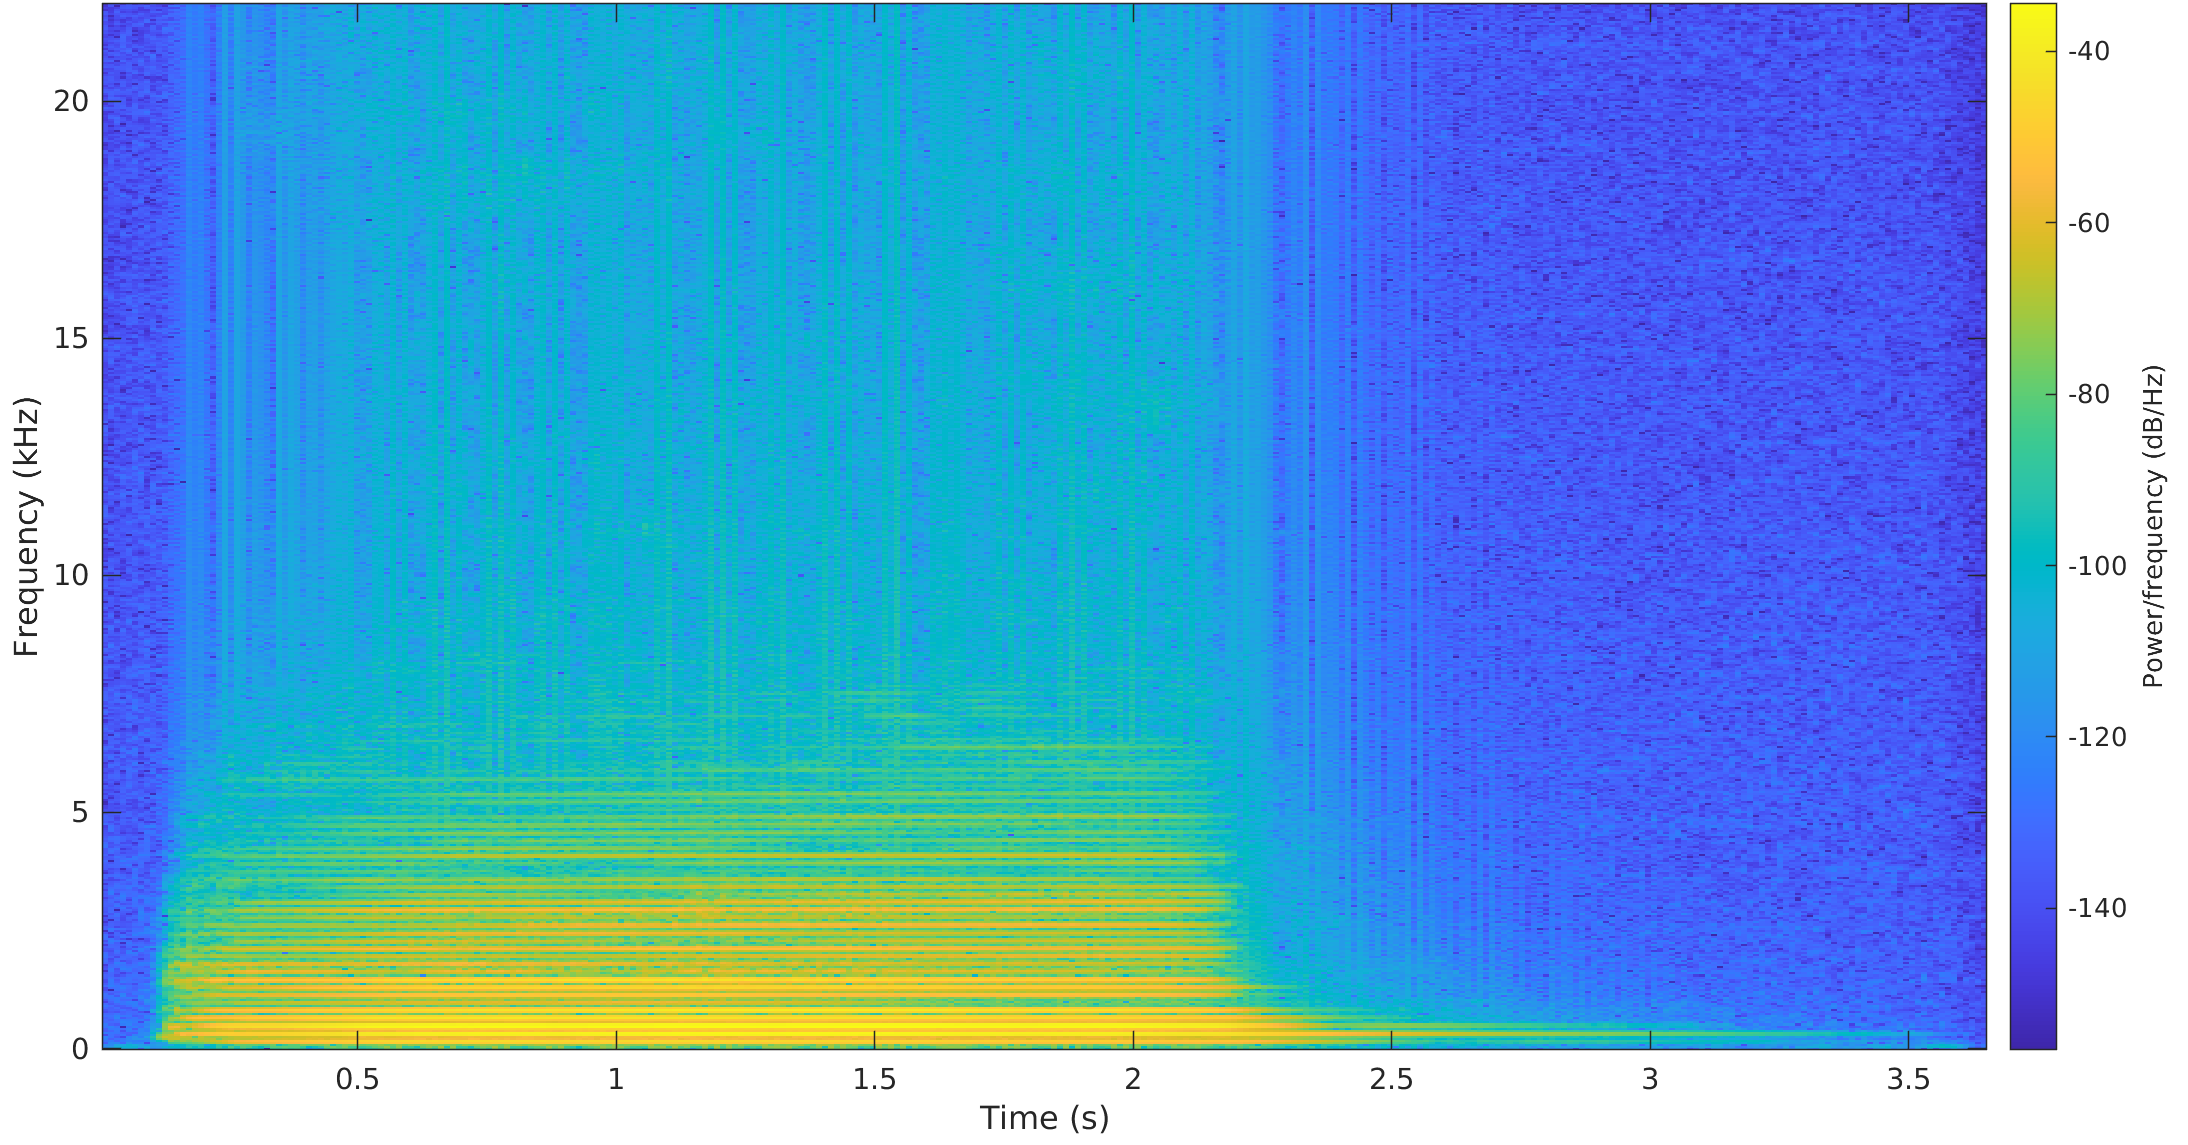
\includegraphics[width=8.5cm]{../images/violaspecgram.png} }}
	\hspace{0.2em}
	\subfloat[Drum spectrogram]{{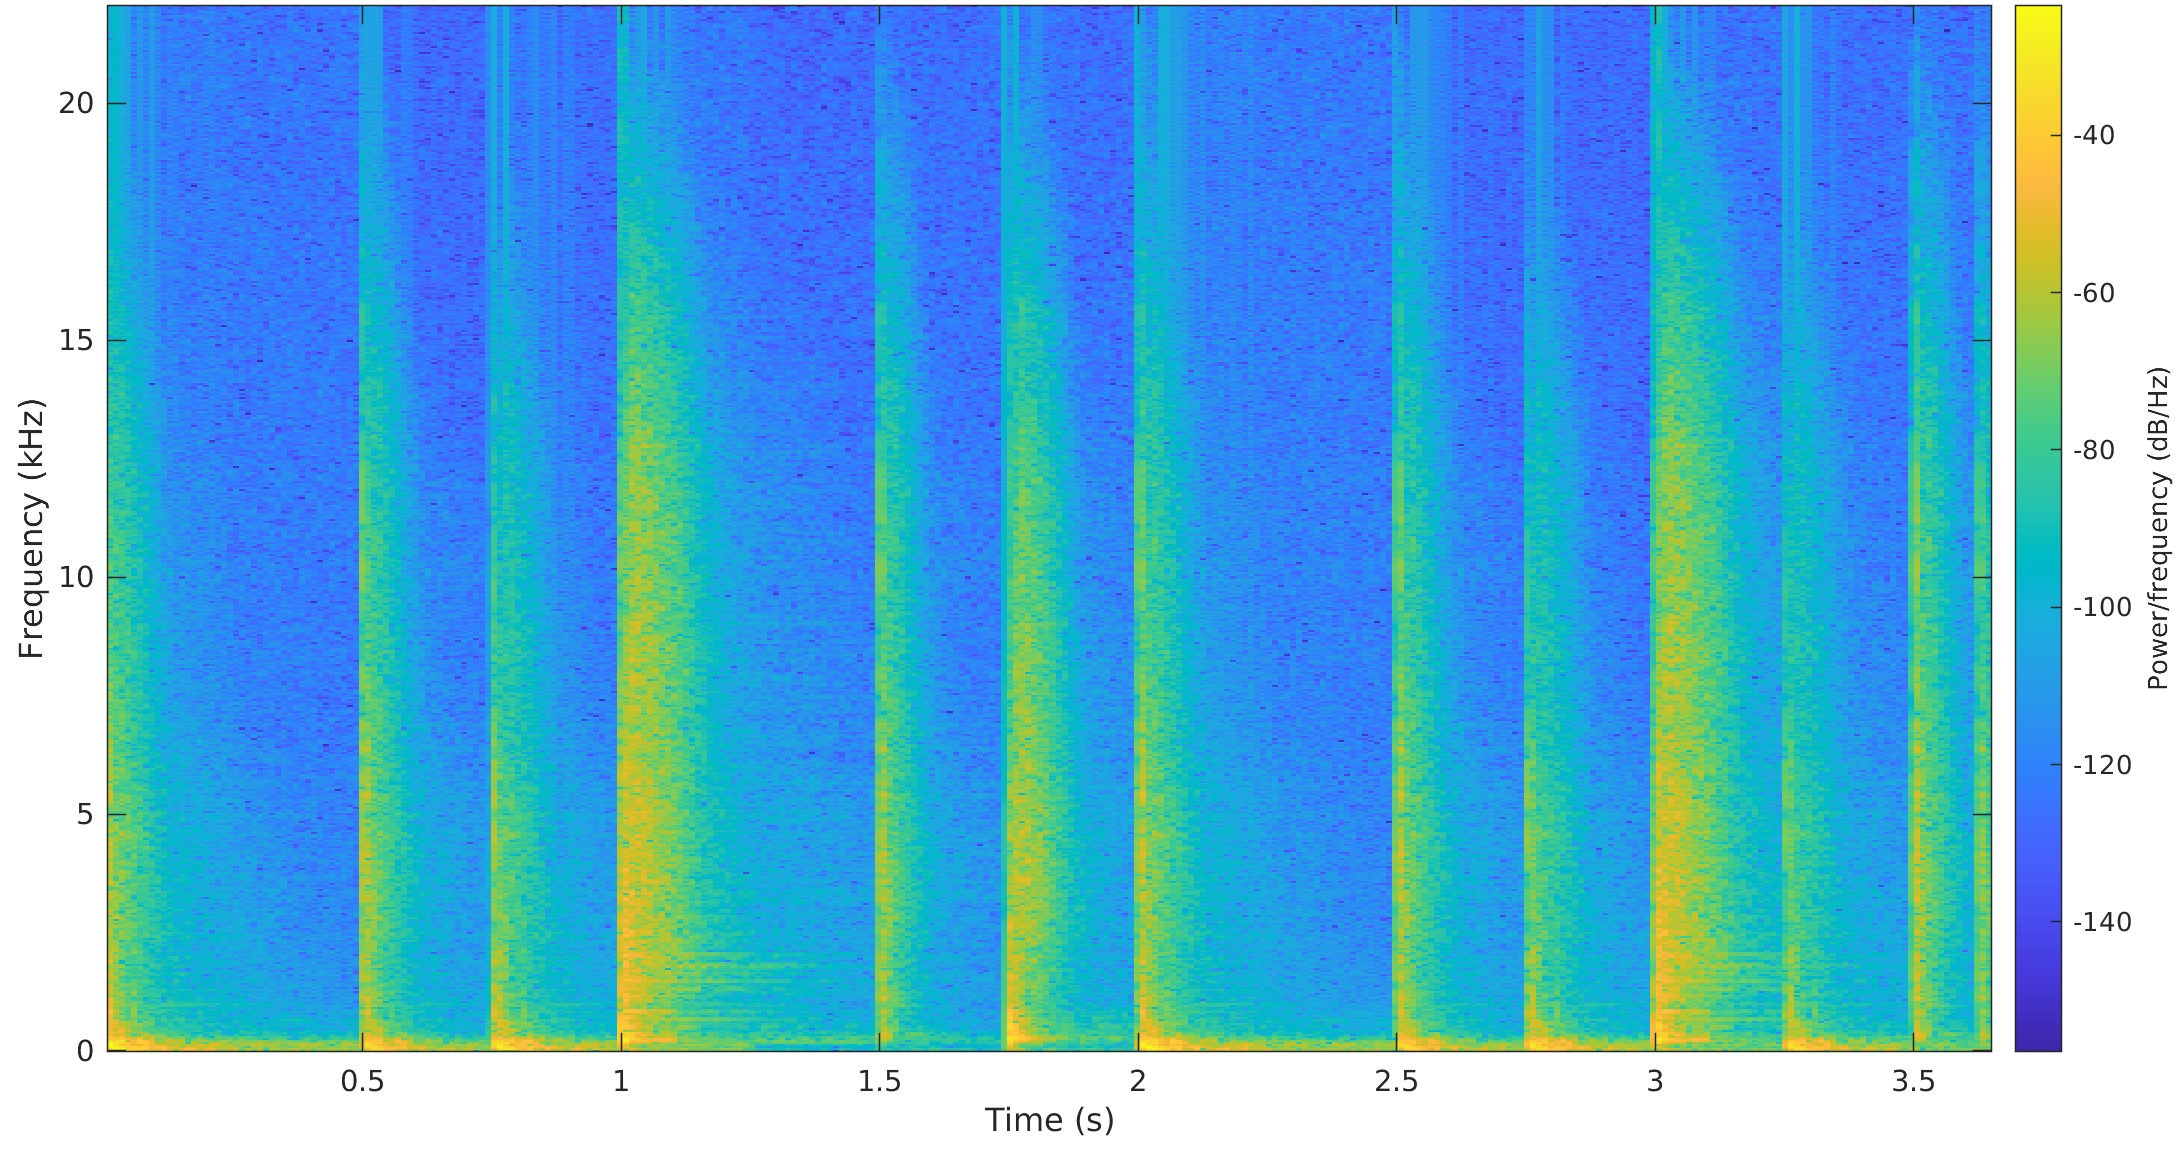
\includegraphics[width=8.5cm]{../images/drumspecgram.png} }}
	\caption{Purely harmonic and purely percussive spectrograms}
	\label{fig:hpspec}%
\end{figure}

Median filtering is a technique from the domain of image processing that is typically used to remove outliers from noisy images \cite{imagenoise}. By performing median filtering in the vertical and horizontal directions (Fitzgerald's technique in \cite{fitzgerald}), we can emphasize the horizontal lines (harmonic) and suppress the vertical sounds (percussive) and vice-versa.

\vfill
\clearpage %force a page break

\section{Background}

\subsection{Median filtering}

It's helpful to first see a simple example of how median filtering works to separate a horizontal and vertical line in Figure~\ref{fig:simplemedfilter}:

\begin{figure}[ht]
	\vspace*{-0.5cm}
	\centering
	\subfloat[Simple image]{{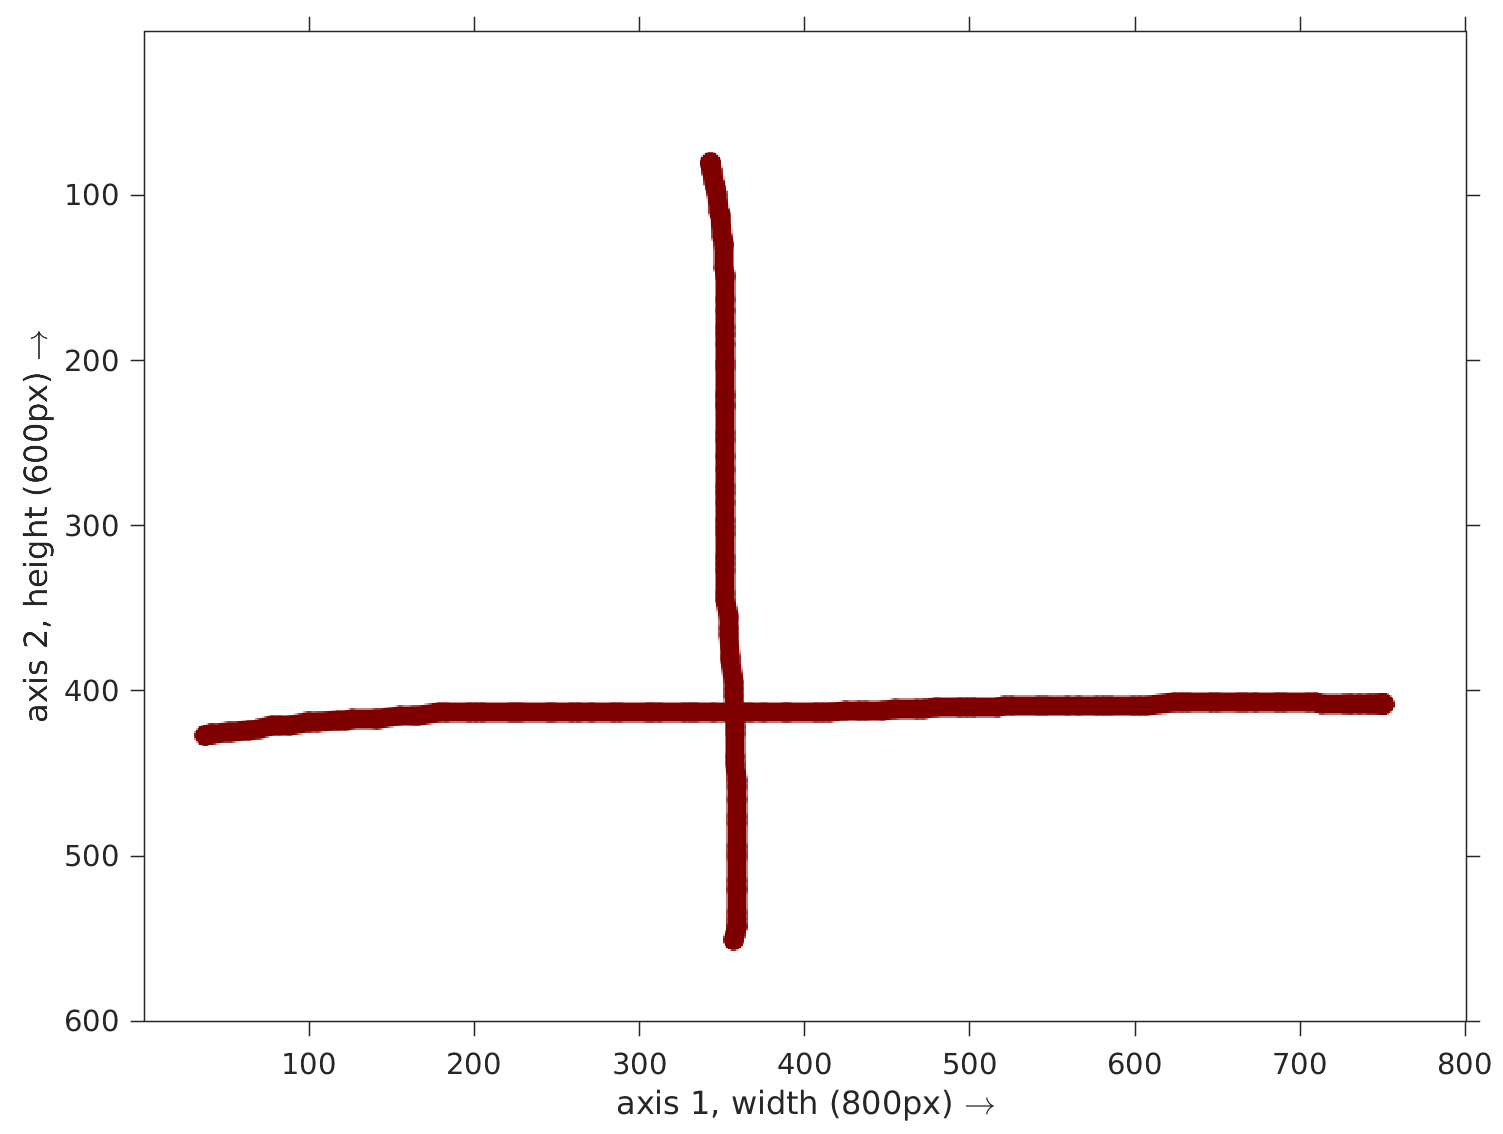
\includegraphics[width=8cm]{../images/medfilter_basic_with_axes.png} }}
	\\
	\subfloat[Median filter, axis 1]{{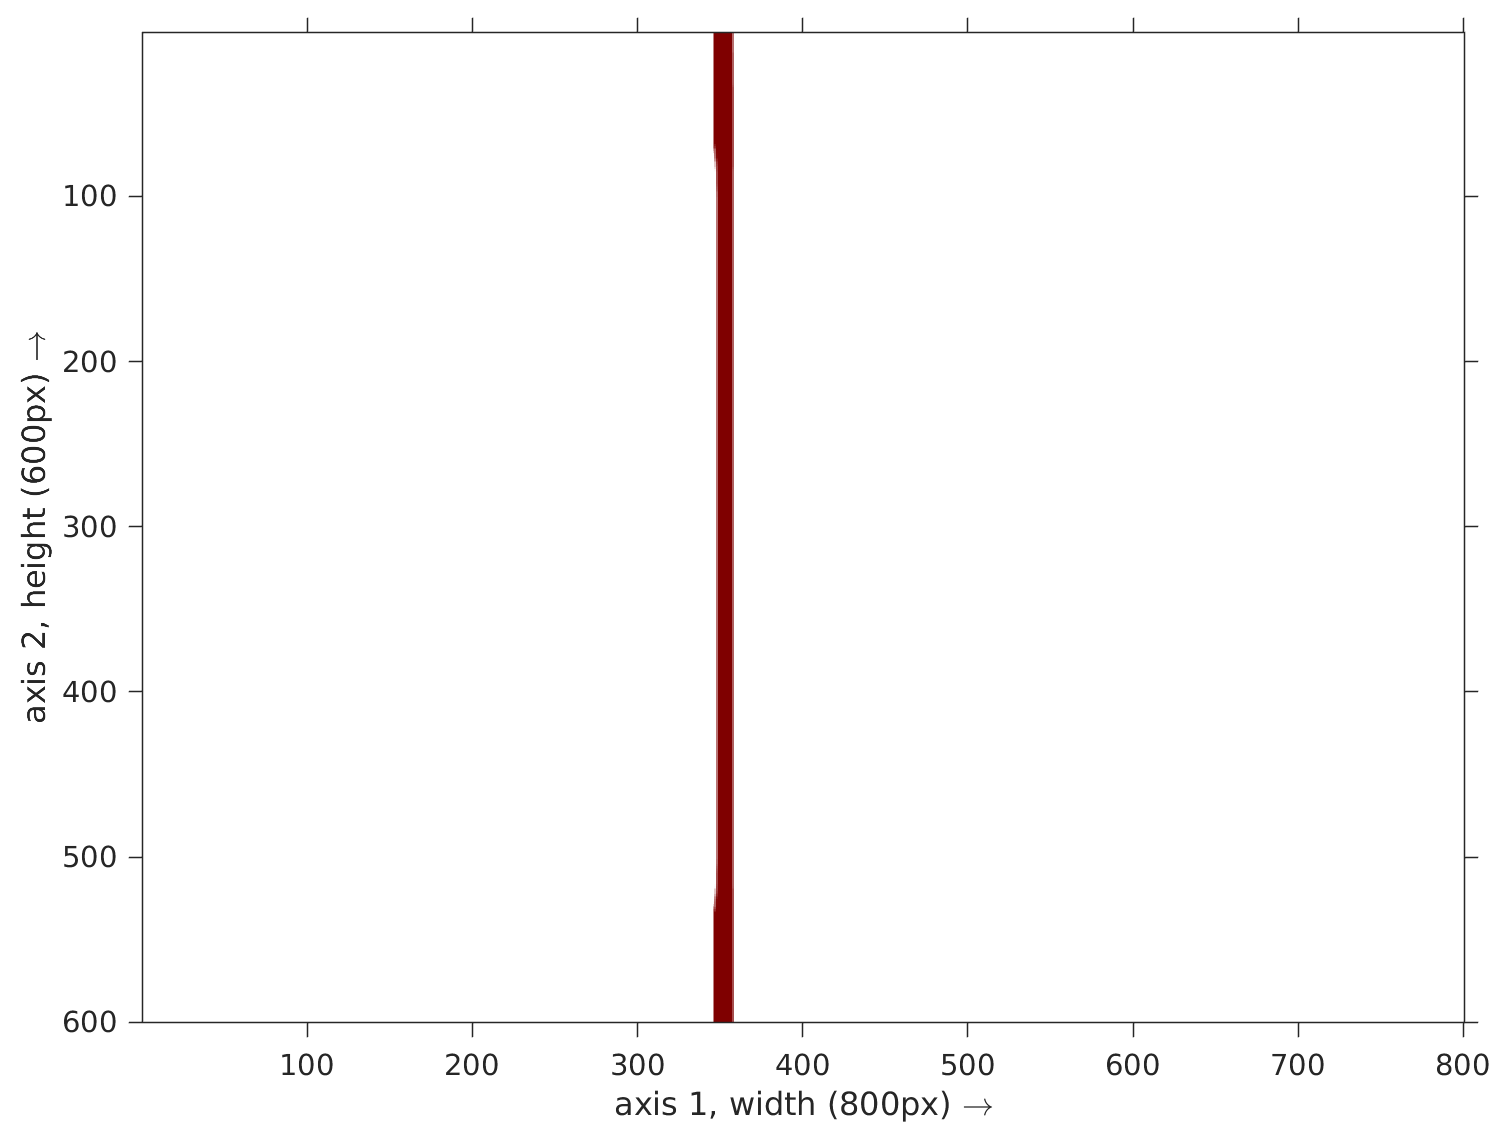
\includegraphics[width=7cm]{../images/medfilter_basic_axis1.png} }}
	\hspace{0.4em}
	\subfloat[Median filter, axis 2]{{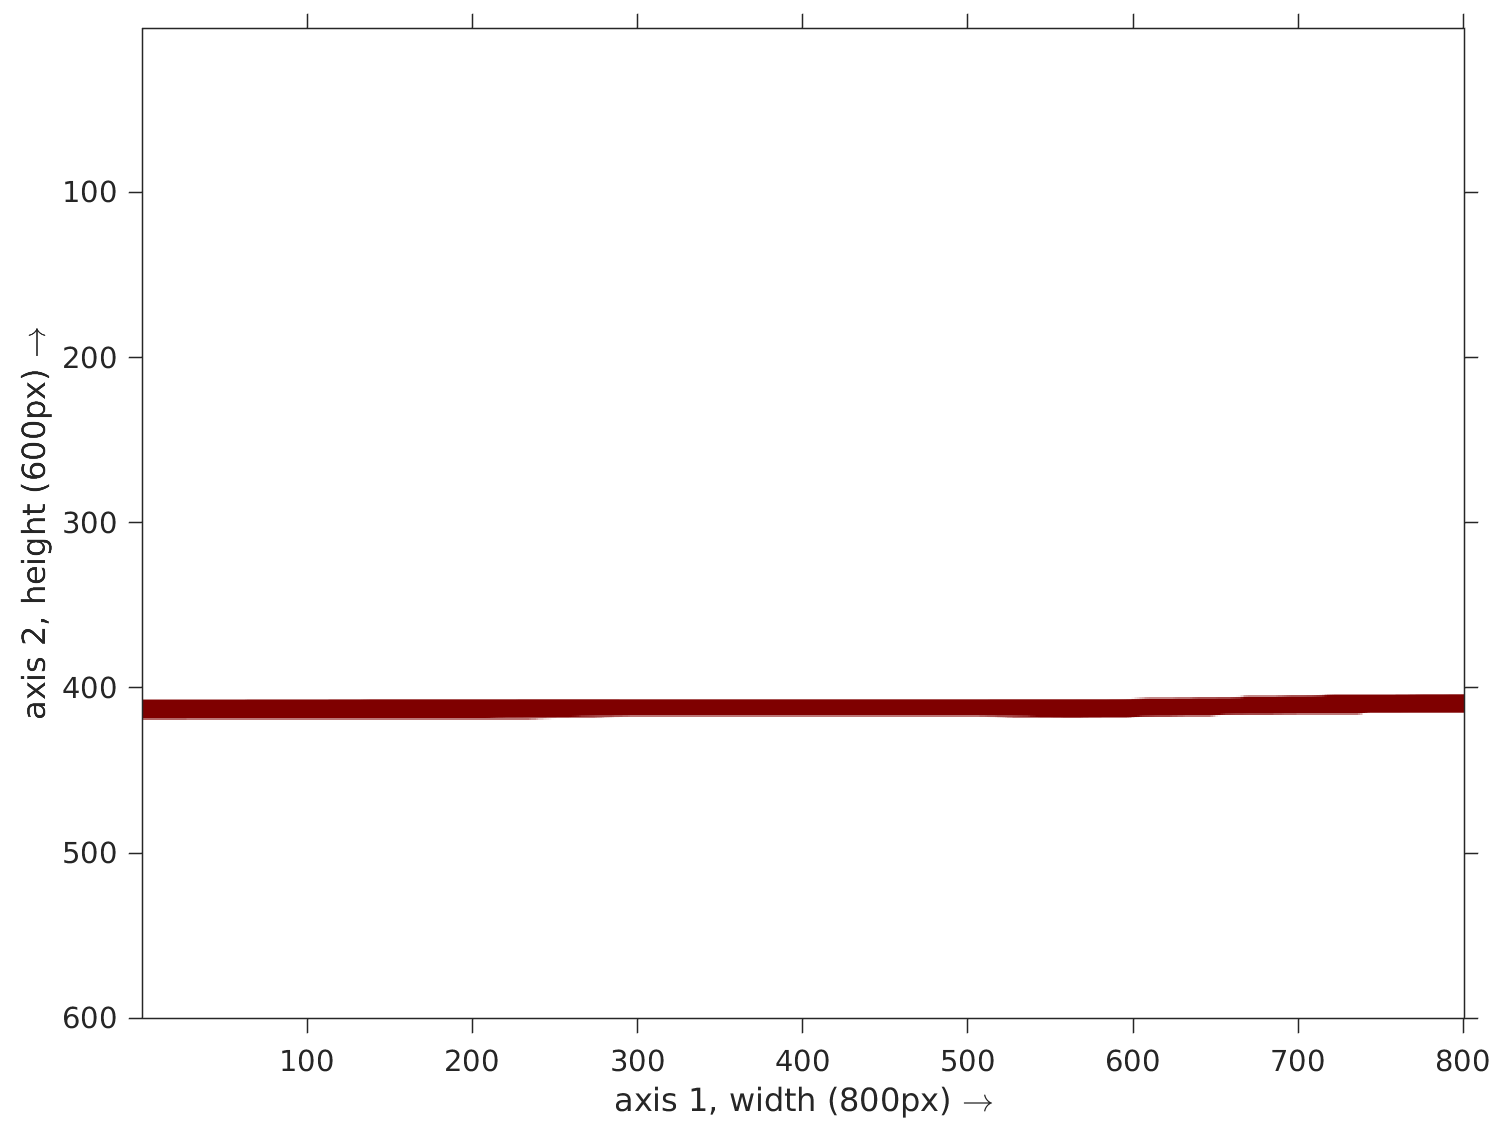
\includegraphics[width=7cm]{../images/medfilter_basic_axis2.png} }}
	\caption{1000-point movmedian applied along axis 1 and 2 on a simple image}%
	\label{fig:simplemedfilter}
\end{figure}

The documentation for ``movmedian'' \cite{movmedian} states this for the dimension argument:

\begin{quote}
M = movmedian(A,k) returns an array of local k-point median values, where each median is calculated over a sliding window of length k across neighboring elements of A . . .\\
M = movmedian(\_\_\_,dim) returns the array of moving medians along dimension dim for any of the previous syntaxes. For example, if A is a matrix, then movmedian(A,k,2) operates along the columns of A, computing the k-element sliding median for each row.
\end{quote}

By executing ``movmedian(imgdata, k, 1)'', the moving median is done along axis 1, or the rows, which computes the k-element sliding median for each column - this emphasizes vertical lines in Figure~\ref{fig:simplemedfilter}b. Similarly, ``movmedian(imgdata, k, 2)'' performs the k-element sliding mean along the columns, emphasizing rows in Figure~\ref{fig:simplemedfilter}c.

\vfill
\clearpage %force a page break

Performing median filtering directly on a PNG image file of the mixed harmonic-percussive spectrogram shows the effectiveness of the algorithm. The results are contained in Figure~\ref{fig:mixspec}. The mixed spectrogram is a spectrogram of the sum of the individual viola and drum waveforms. The median filtering is done with the MATLAB code in Listing~\ref{code:medfilterim}.

\begin{figure}[ht]
	\vspace*{-0.5cm}
	\centering
	\subfloat[Mixed harmonic-percussive spectrogram]{{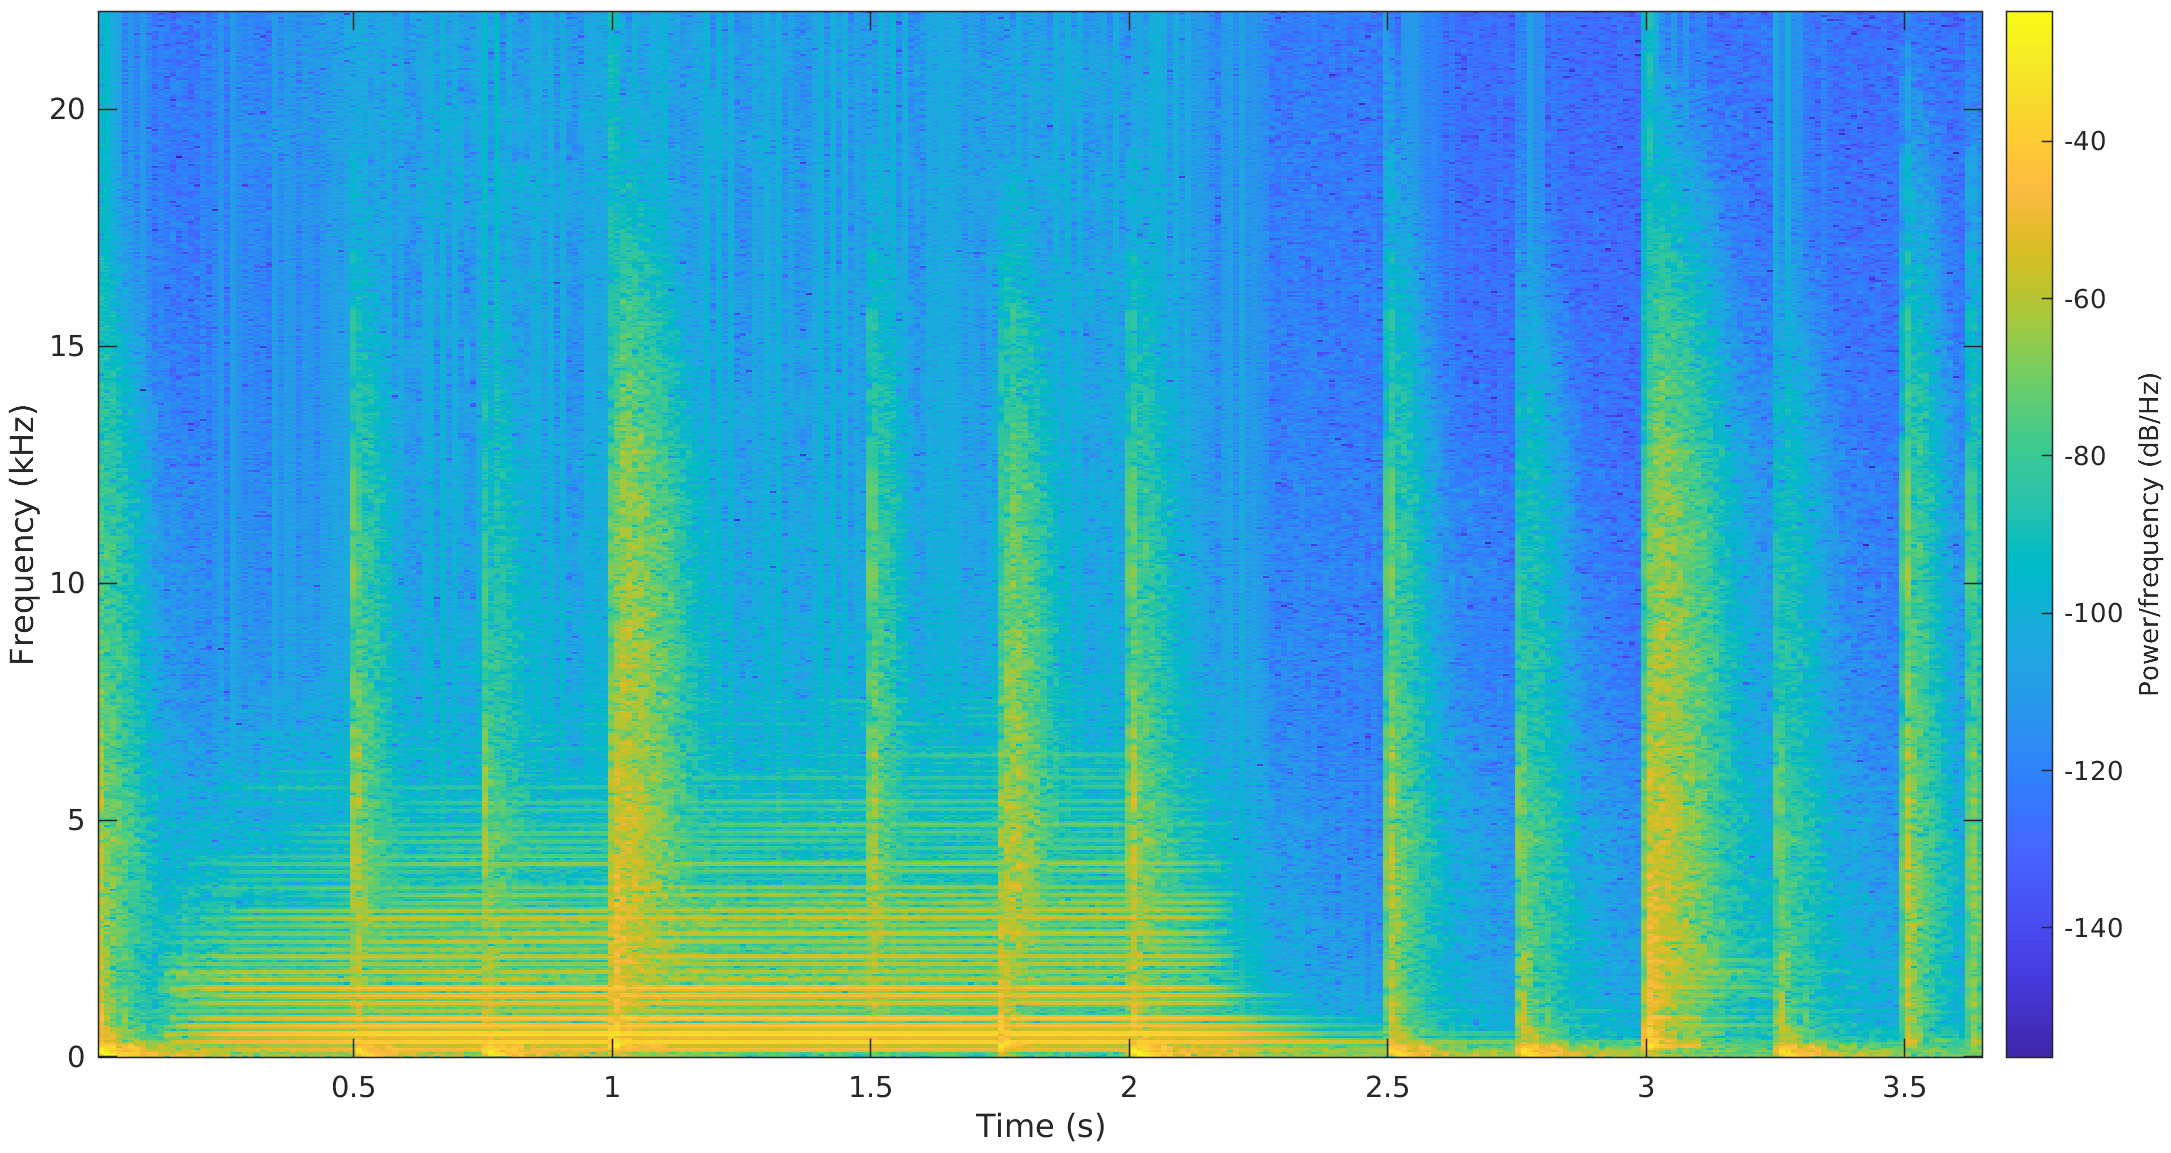
\includegraphics[width=8cm]{../images/mixedspecgram.png} }}
	\hspace{0.4em}
	\subfloat[Left with axes and labels cropped]{{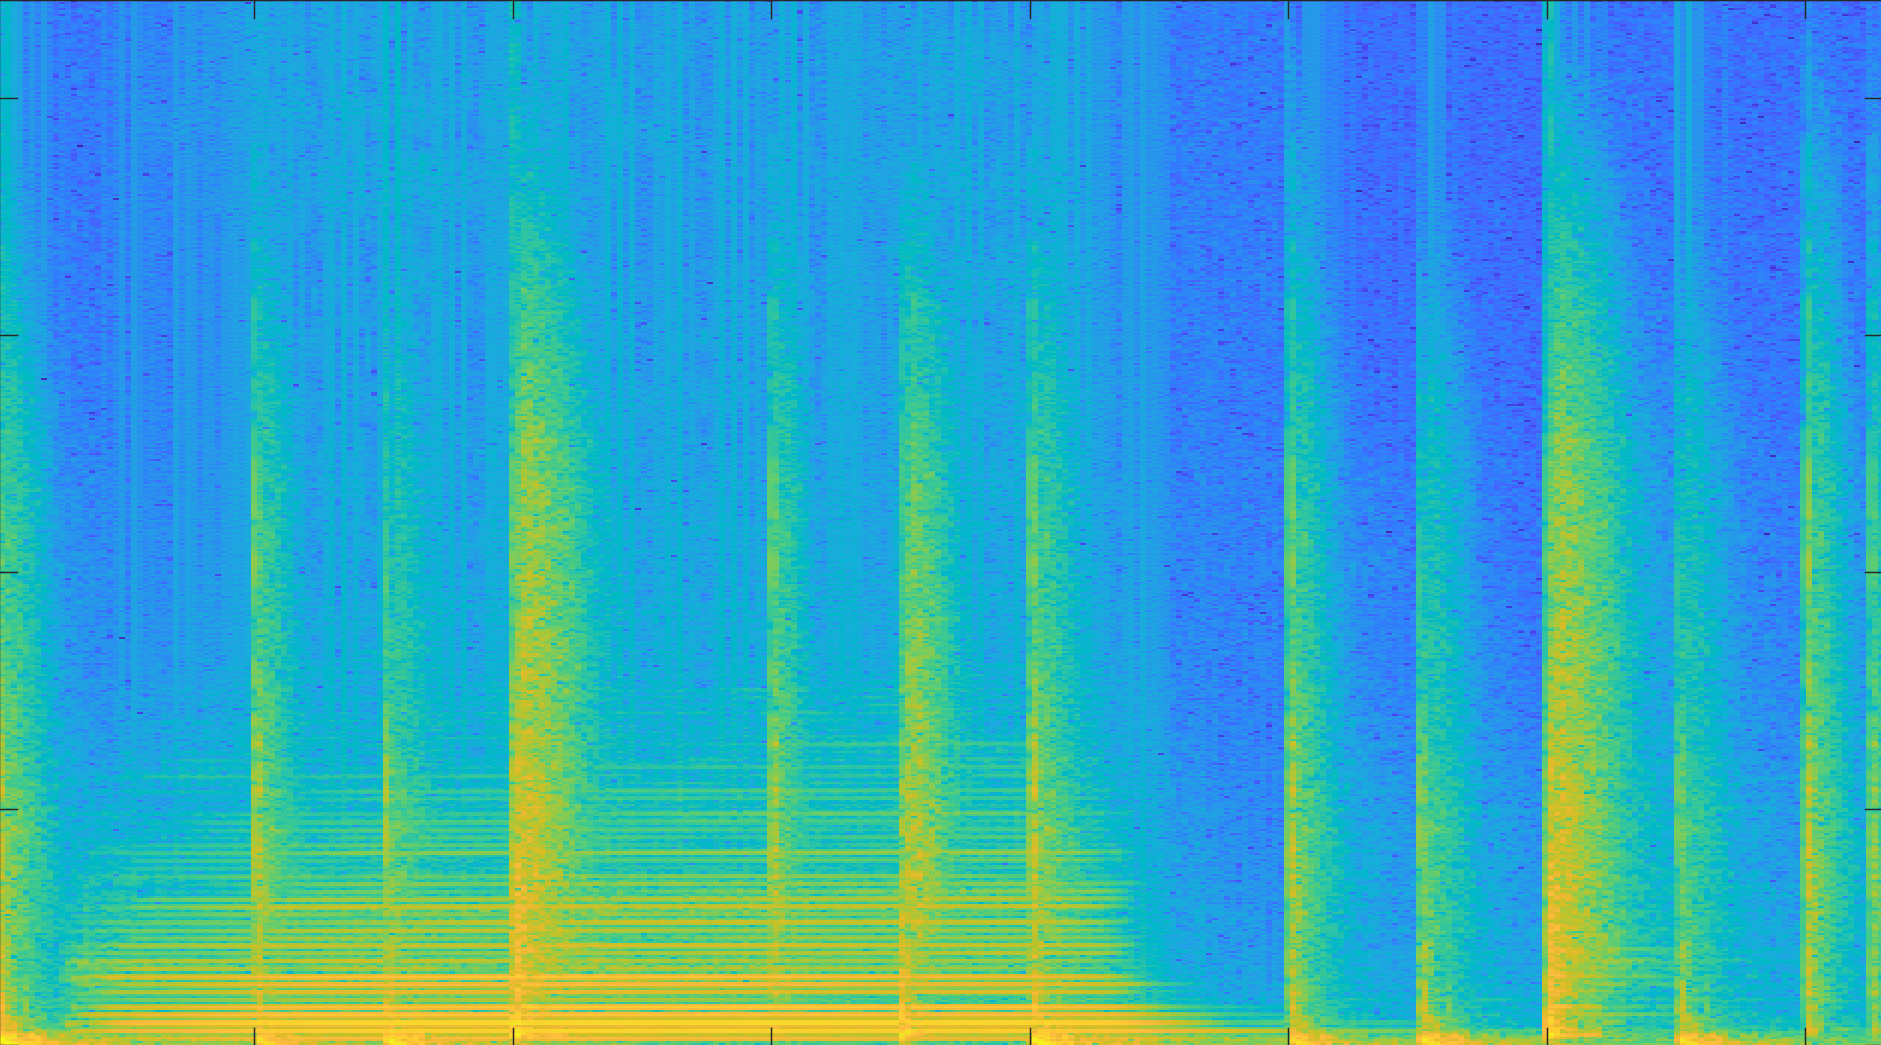
\includegraphics[width=8cm]{../images/mixedspecgram_cropped.png} }}
	\\
	\subfloat[Median filter, axis 1]{{
\includegraphics[width=8cm]{../images/medfilter_axis1.png} }}
	\hspace{0.4em}
	\subfloat[Median filter, axis 2]{{
\includegraphics[width=8cm]{../images/medfilter_axis2.png} }}
	\\
	\subfloat[Original drum spectrogram, cropped]{{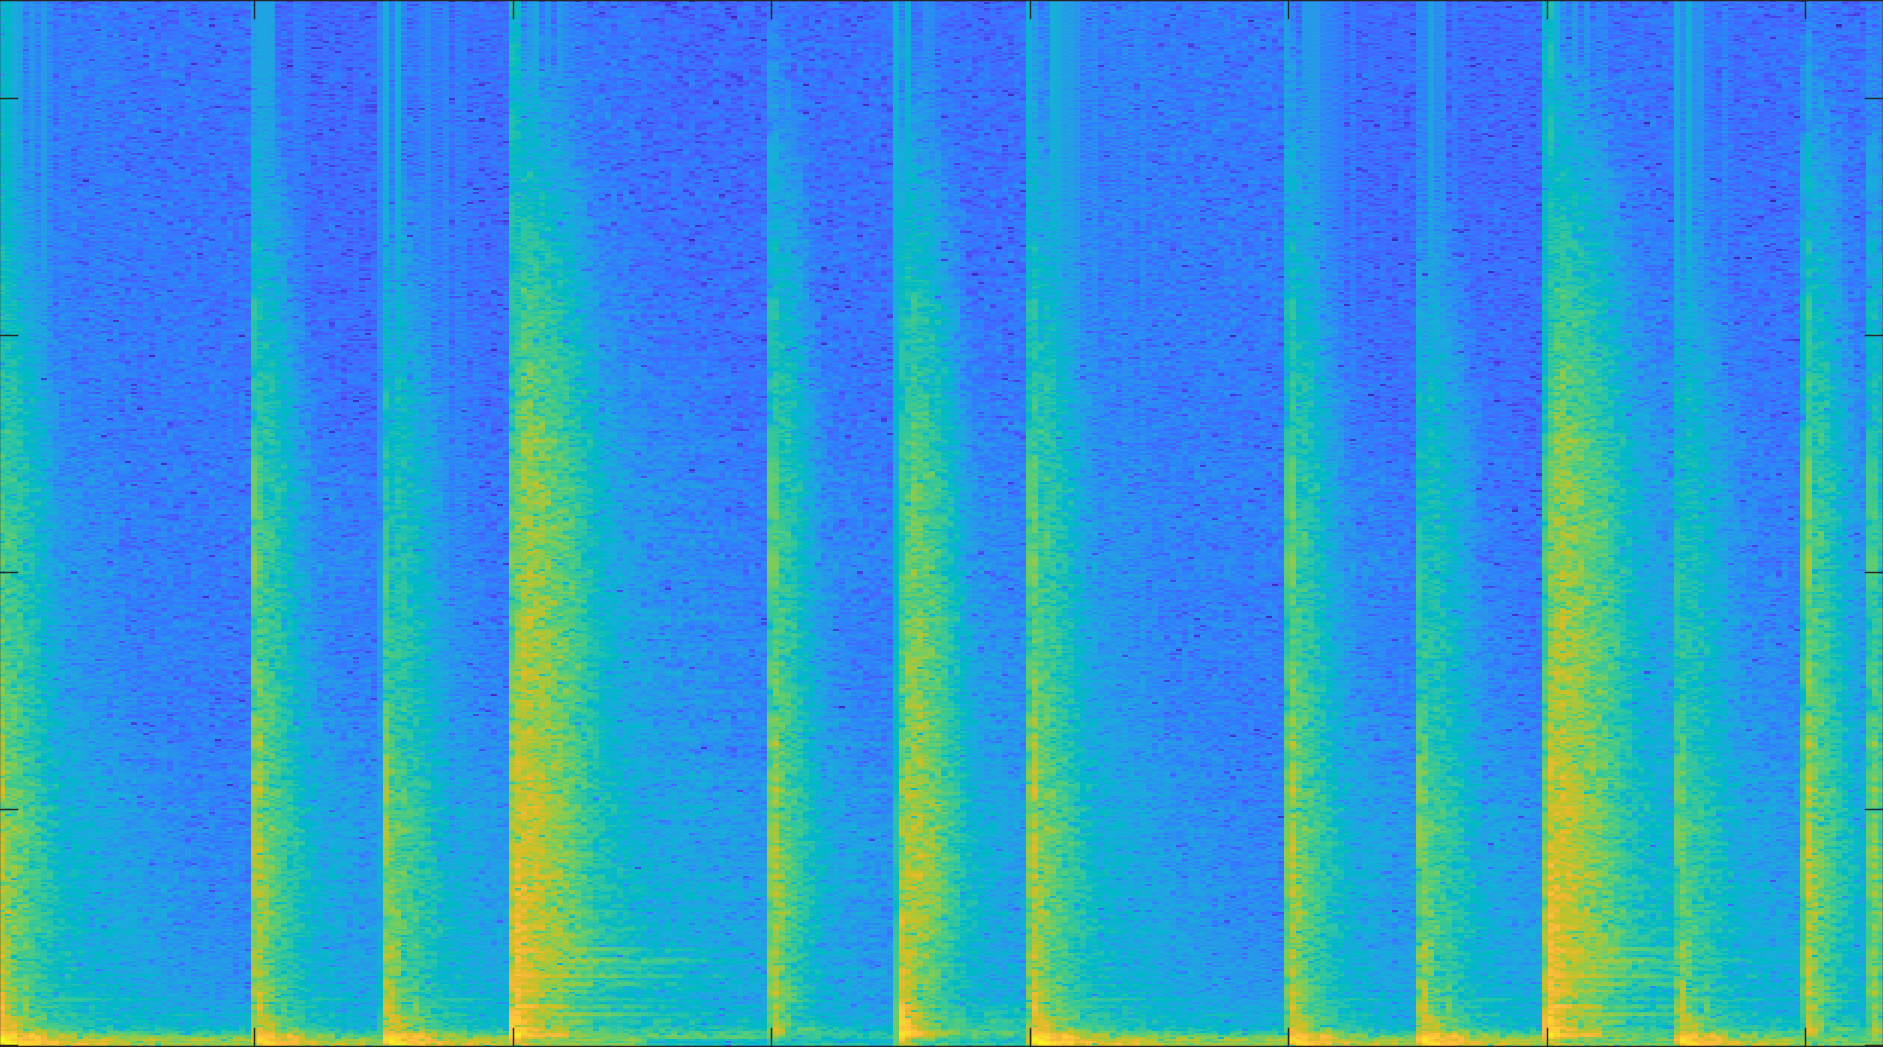
\includegraphics[width=8cm]{../images/drumspecgram_orig.png} }}
	\hspace{0.4em}
	\subfloat[Original viola spectrogram, cropped]{{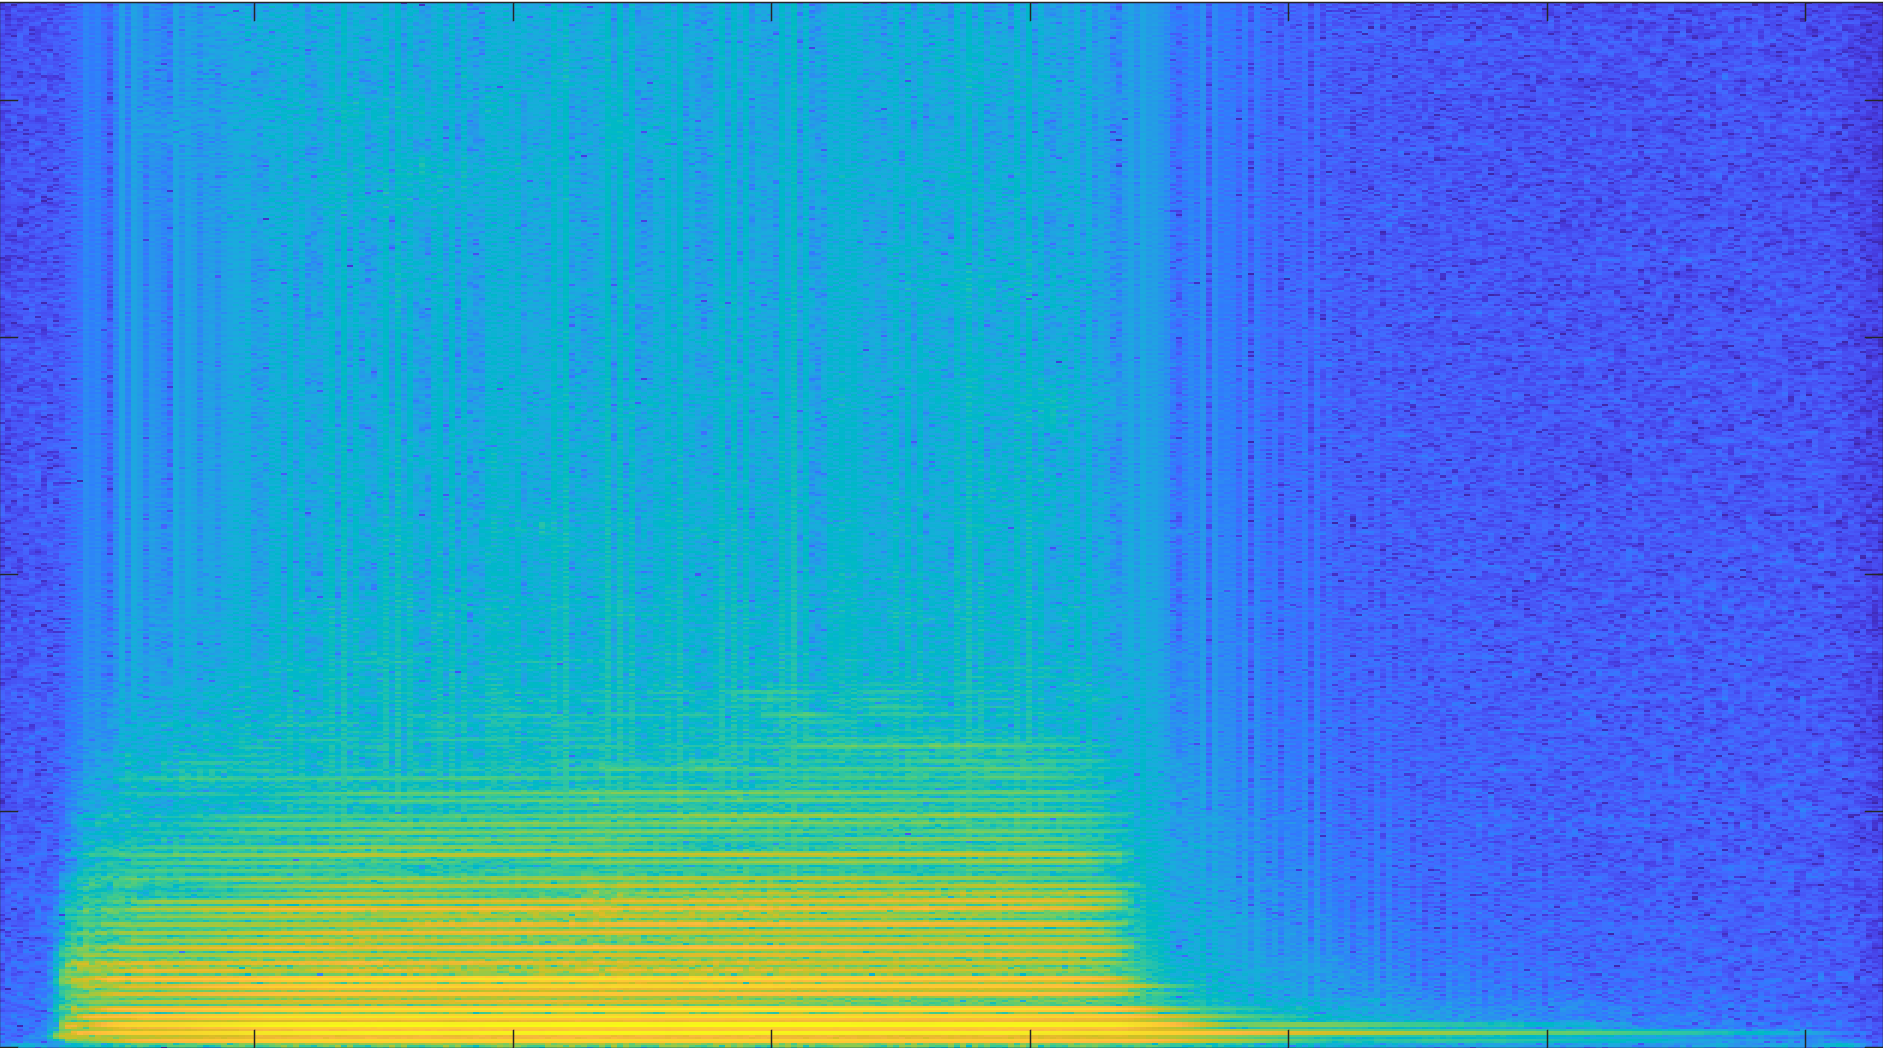
\includegraphics[width=8cm]{../images/violaspecgram_orig.png} }}
	\caption{Horizontal and vertical median filter applied on a mixed harmonic-percussive spectrogram}
	\label{fig:mixspec}%
\end{figure}

\begin{listing}[h]
\setlength\partopsep{-\topsep}
\begin{minted}[breaklines,linenos,frame=single,fontsize=\small,linenos]{matlab}
x = imread("mixedspecgram_cropped.png");
x_h = movmedian(x, 1000, 1);
x_p = movmedian(x, 1000, 2);
imwrite(x_h, "medfilter_axis1.png");
imwrite(x_p, "medfilter_axis2.png");
\end{minted}
\caption{MATLAB image median filtering}
\label{code:medfilterim}
\end{listing}

\vfill
\clearpage %force a page break

\subsection{Time-frequency analysis, the spectrogram, and the STFT}

The MATLAB spectrogram plot uses the STFT \cite{specstft}. The short-time Fourier transform, or STFT, is a sequence of DFTs of a signal split into time-localized segments, for situations in which frequency components of a signal vary over time \cite{timefreq}. When the DFT is applied to consecutive segments of an input signal, this can create spectral leakage \cite{whyoverlap}:

\begin{quote}
	[T]he DFT implicitly assumes that the signal is periodic... If the frequency of the sinusoidal input signal is not an exact multiple of the frequency resolution, this assumption is not true, and the DFT will see a discontinuity between the last sample and the first sample due to the cyclic continuation. That discontinuity spreads power all across the spectrum.
\end{quote}

The reason there is windowing and overlapping in the STFT is to reduce the effect of spectral leakage. By applying a tapering window, we are eliminating the spectral leakage discontinuities at the boundaries, but also losing data. We want segments to overlap to preserve the lost data:

\begin{figure}[ht]
	\vspace*{-0.15cm}
	\centering
	\subfloat[A visualization of spectral leakage \cite{leakage}]{{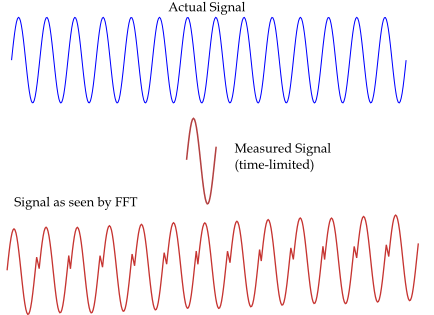
\includegraphics[height=5cm]{../images/spectral_leakage.png} }}
	\hspace{0.2em}
	\subfloat[von Hann window with tapered boundaries]{{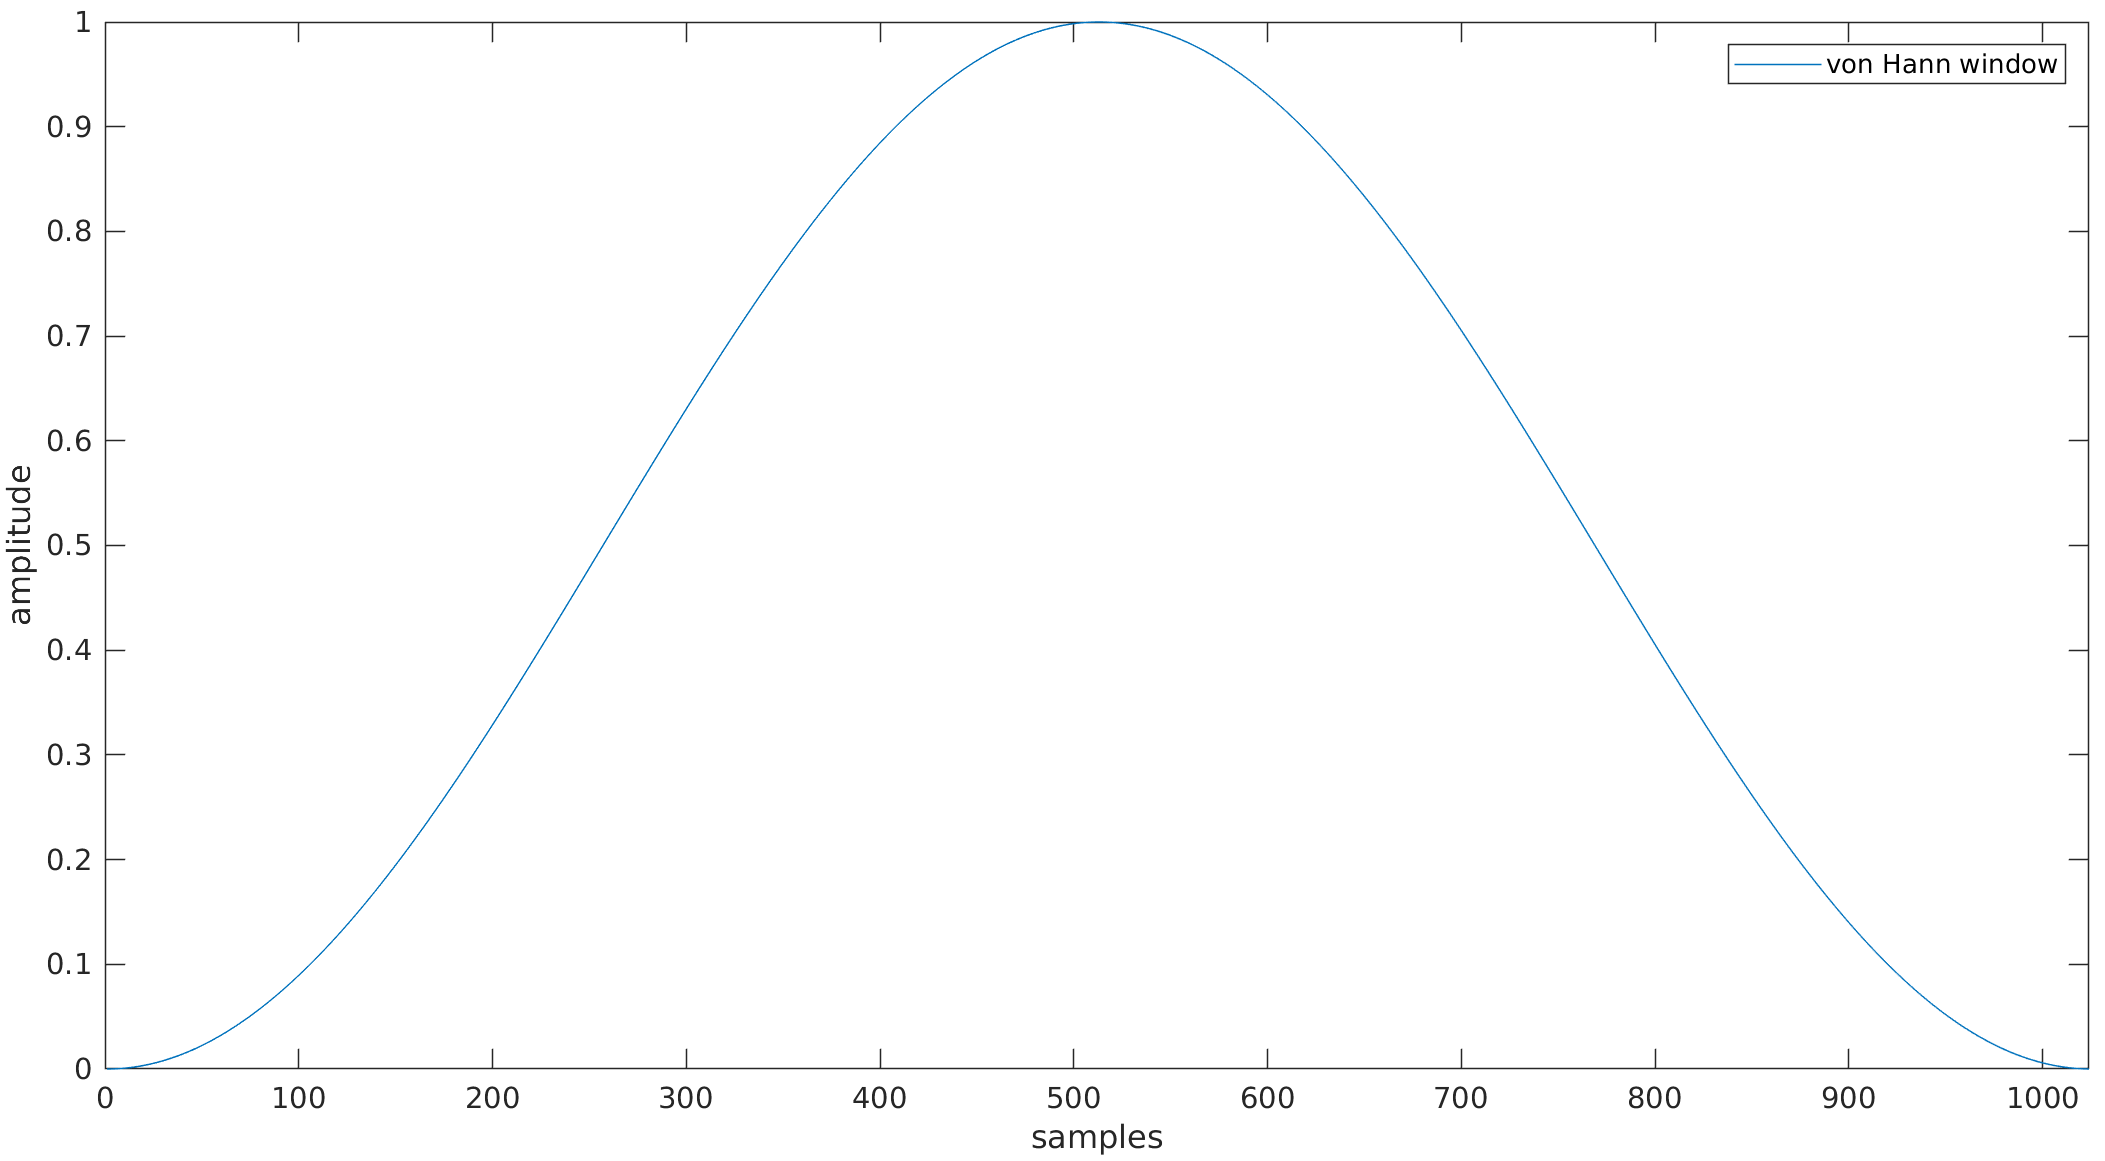
\includegraphics[width=8.5cm]{../images/hann_taper_window.png} }}
	\\
	\subfloat[Data loss at boundaries]{{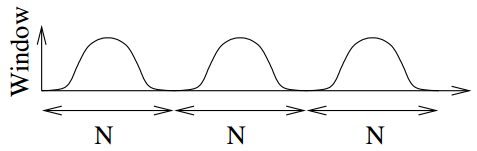
\includegraphics[width=8.5cm]{../images/whyoverlap1.png} }}
	\hspace{0.2em}
	\subfloat[Overlap to preserve data]{{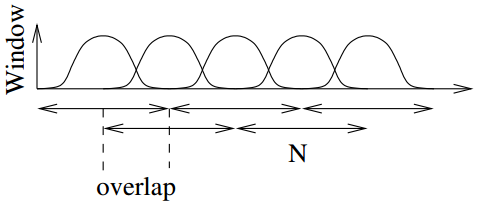
\includegraphics[width=8.5cm]{../images/whyoverlap2.png} }}
	\caption{Spectral leakage, windowing, and overlapping}
	\label{fig:whyoverlap}%
\end{figure}

\subsection{Time-frequency masking}

Time-frequency masking (T-F masking) is a common technique for source separation \cite{wang2008time}, \cite{timefreq2}. The technique involves creating 2-dimensional masks to apply to the time-frequency representation of sound to separate the target signal from the interfering signals. If the mask coefficients are only 0 and 1, this is known as binary masking -- otherwise, the T-F mask is a ratio mask, soft mask, or Wiener filter. Wiener filters are also used in image processing \cite{wienernoise}, applied in the frequency domain to separate signal from noise.

\section{Median-filtering HPSS}

Enough background has been presented to be able to describe a pseudocode implementation of the original 2010 median-filtering HPSS algorithm in Listing~\ref{code:fitzpseudo}:

\begin{listing}[h]
\setlength\partopsep{-\topsep}
\begin{minted}[linenos,mathescape=true,breaklines,frame=single,escapeinside=||]{text}
|$ s = \text{mixed audio}, \hat{S} = \text{STFT}(s), S = \text{abs}(\hat{S}) $|
|$ H = \text{medianfilter}(S, l_{H}, \text{axis}=2), P = \text{medianfilter}(S, l_{P}, \text{axis}=1) $|
|$ M_{H} = \frac{H^{p}}{H^{p} + P^{p}}, M_{P} = \frac{P^{p}}{H^{p} + P^{p}}$|
|$\hat{H} = \hat{S} \cdot M_{H}, \hat{P} = \hat{S} \cdot M_{P} $|
|$h = \text{ISTFT}(\hat{H}), p = \text{ISTFT}(\hat{P}) $|
\end{minted}
\caption{Fitzgerald median-filtering HPSS pseudocode}
\label{code:fitzpseudo}
\end{listing}

 In step 3, soft masks raised to the $p$th power are computed to separate the percussive parts of the signal $\hat{S} = \hat{H} + \hat{P}$ to recover the harmonic, and vice-versa. Driedger et al. in 2014 \cite{driedger} propose that there is some additional residual component $\hat{R}$ which is neither harmonic nor percussive, such that $\hat{S} = \hat{H} + \hat{P} + \hat{R}$,. It is introduced with a new parameter $\beta$, the separation factor, which replaces the Fitzgerald soft masks with binary masks in (1):

 \setlength{\abovedisplayskip}{0pt}%
 \setlength{\abovedisplayshortskip}{0pt}%
 \begin{align}
	 \vspace{-1em}
		M_{h} = \frac{H}{P + \epsilon} > \beta, M_{p} = \frac{P}{H + \epsilon} \ge \beta, M_{r} = 1 - (M_{h} + M_{p})
 \end{align}

$\epsilon$ is to avoid division by 0. Note that even if we don't care to use the residual $\hat{R}$, $\hat{H}$ and $\hat{P}$ have a better separation. There is also a proposed iterative variant which first processes the input signal spectrogram with $N = 4096$ to produce good harmonic separation, then does a second pass with $N = 256$ to produce good percussive separation. We'll implement the single-pass variant because it is more similar to the Fitzgerald algorithm, allowing a fair comparison. Also, the single-pass variant with a frame size of $N = 1024$ has lower computational cost and latency, making it more appropriate for real-time.

\subsection{MATLAB implementation and results}

The results of the implementation from the same viola and drum clips seen throughout this report are in Figures \ref{fig:harmwaveformresult}-\ref{fig:percspecresult}. The HPSS function used to generate those results is in Listing~\ref{code:fullimpl}, shown after the figures. Lines 20--23 in Listing~\ref{code:fullimpl} contain the Driedger et al. binary mask computation with the separation factor $\beta = 2$, and lines 25--28 contain the Fitzgerald soft mask raised to the $p$th power, $p = 2$. You may notice the characteristic of binary vs. soft masking in how the binary-masked spectrograms contain discontinuities/holes/silences where the separation was done, while the soft-masked spectrograms look more natural.\\

An additional implementation detail is that the masks are computed from the magnitude of half of the STFT. This is because the second half of each DFT is redundant, and the magnitude information is more important than the phase which the human ear is less sensitive to \cite{zafar}.

\begin{figure}[ht]
	\centering
	\subfloat[Original mixed waveform]{{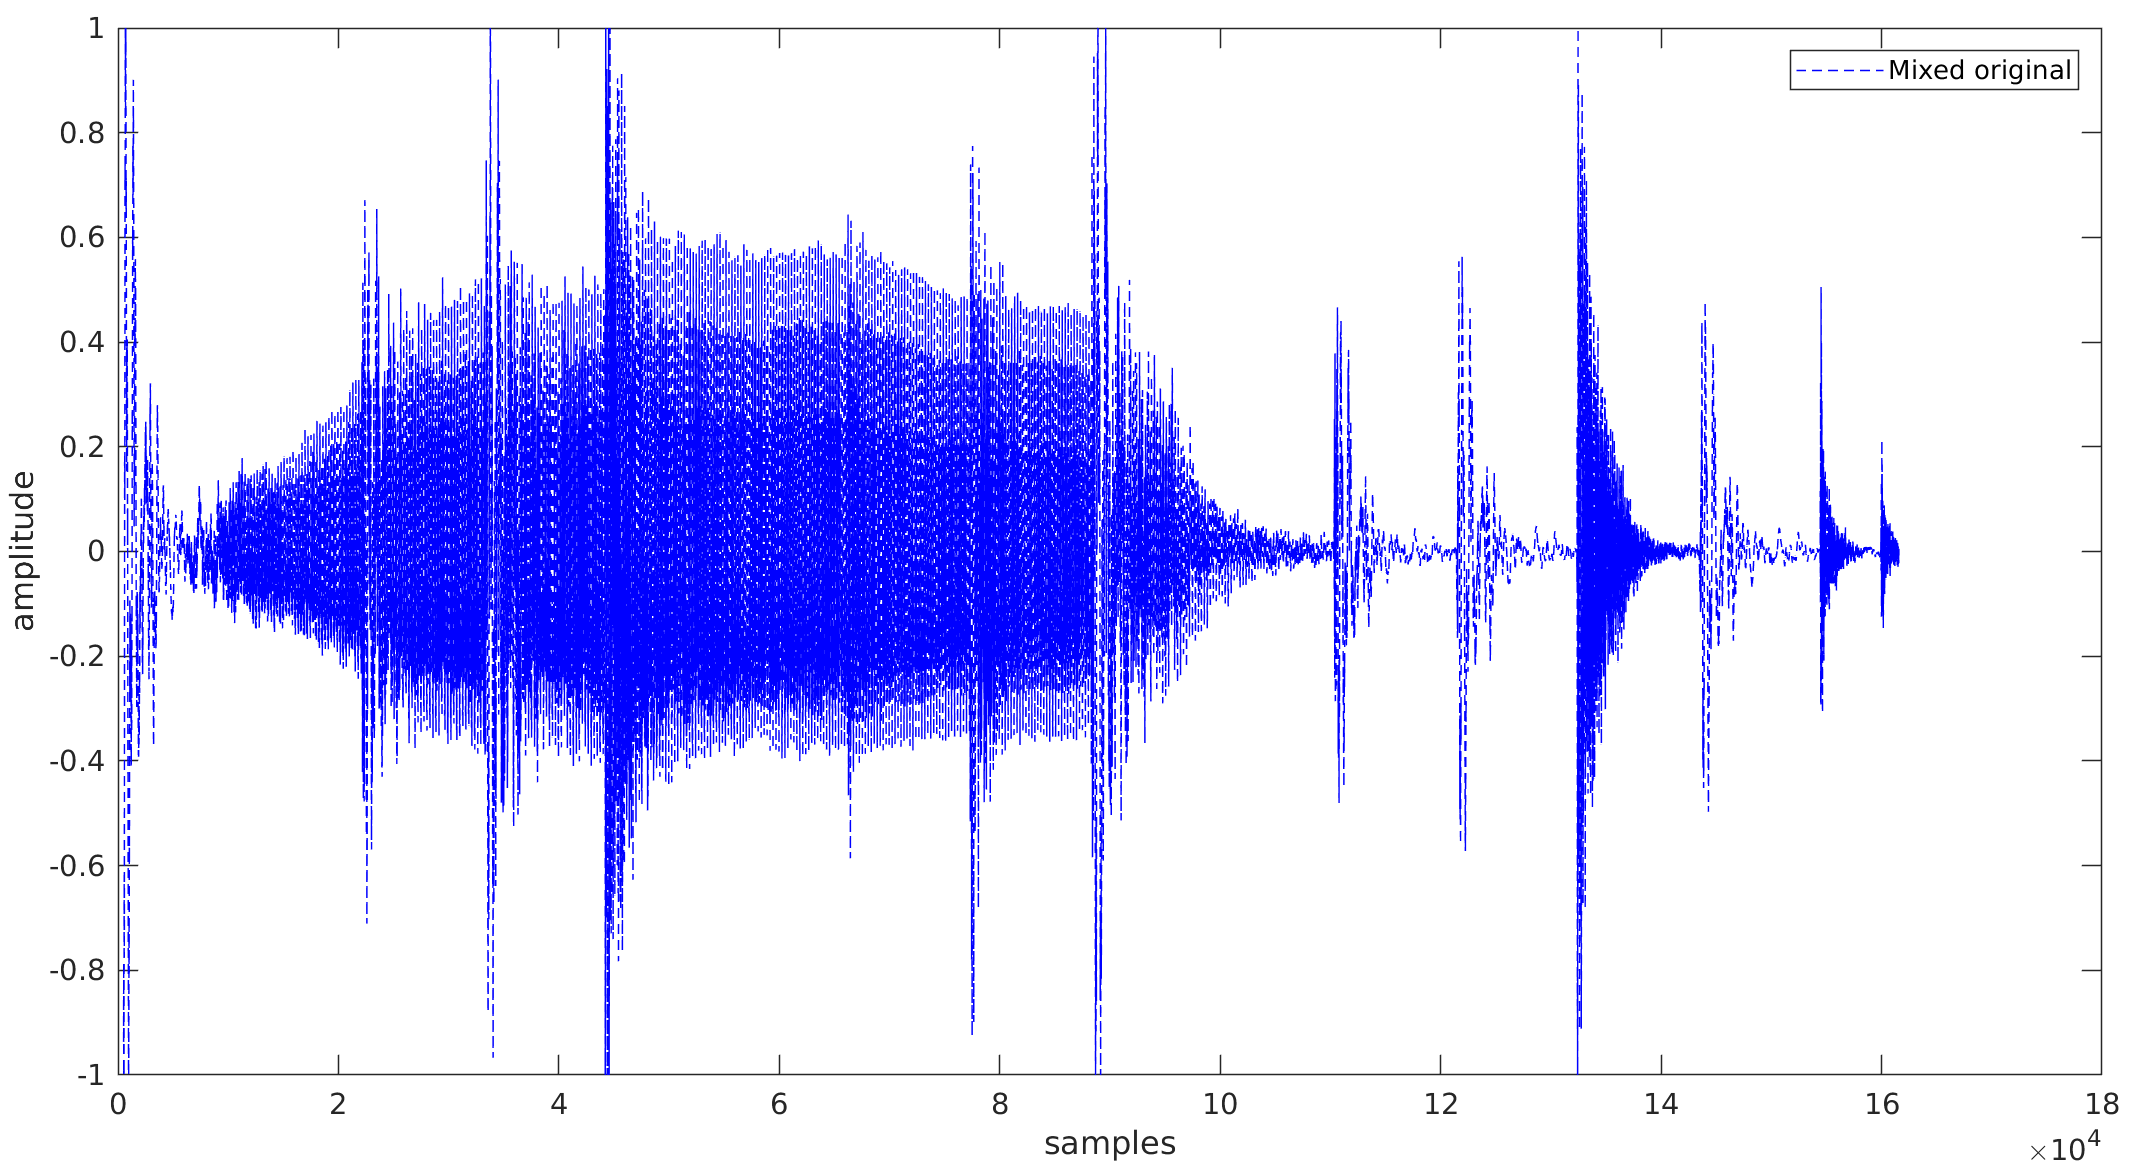
\includegraphics[width=12cm]{../images/waveform_realtime_orig.png} }}
	\\
	\subfloat[Harmonic separated vs. original, soft mask]{{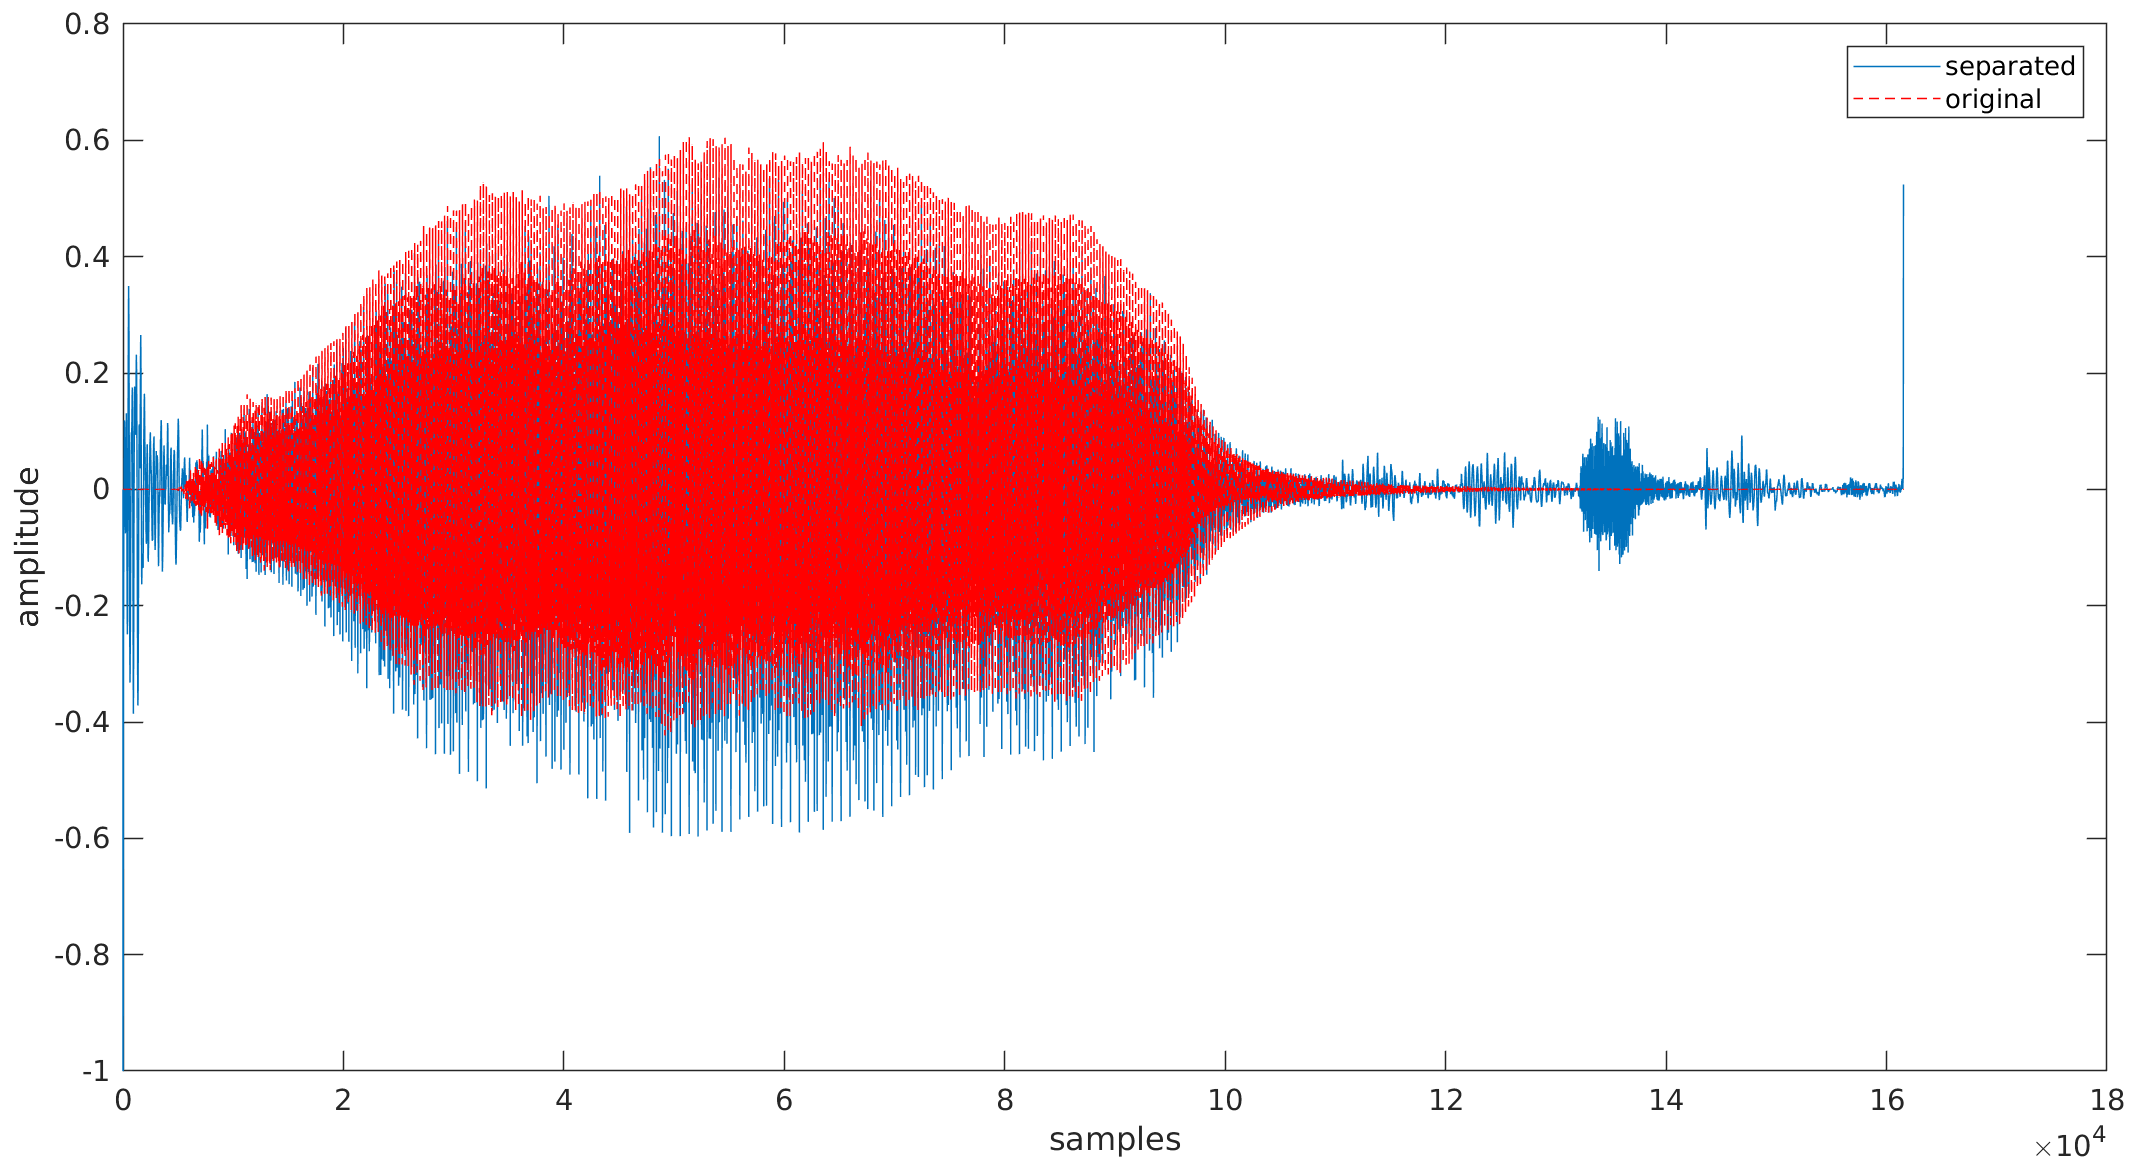
\includegraphics[width=12cm]{../images/harm_fitzgerald_cmp.png} }}
	\\
	\subfloat[Harmonic separated vs. original, binary mask]{{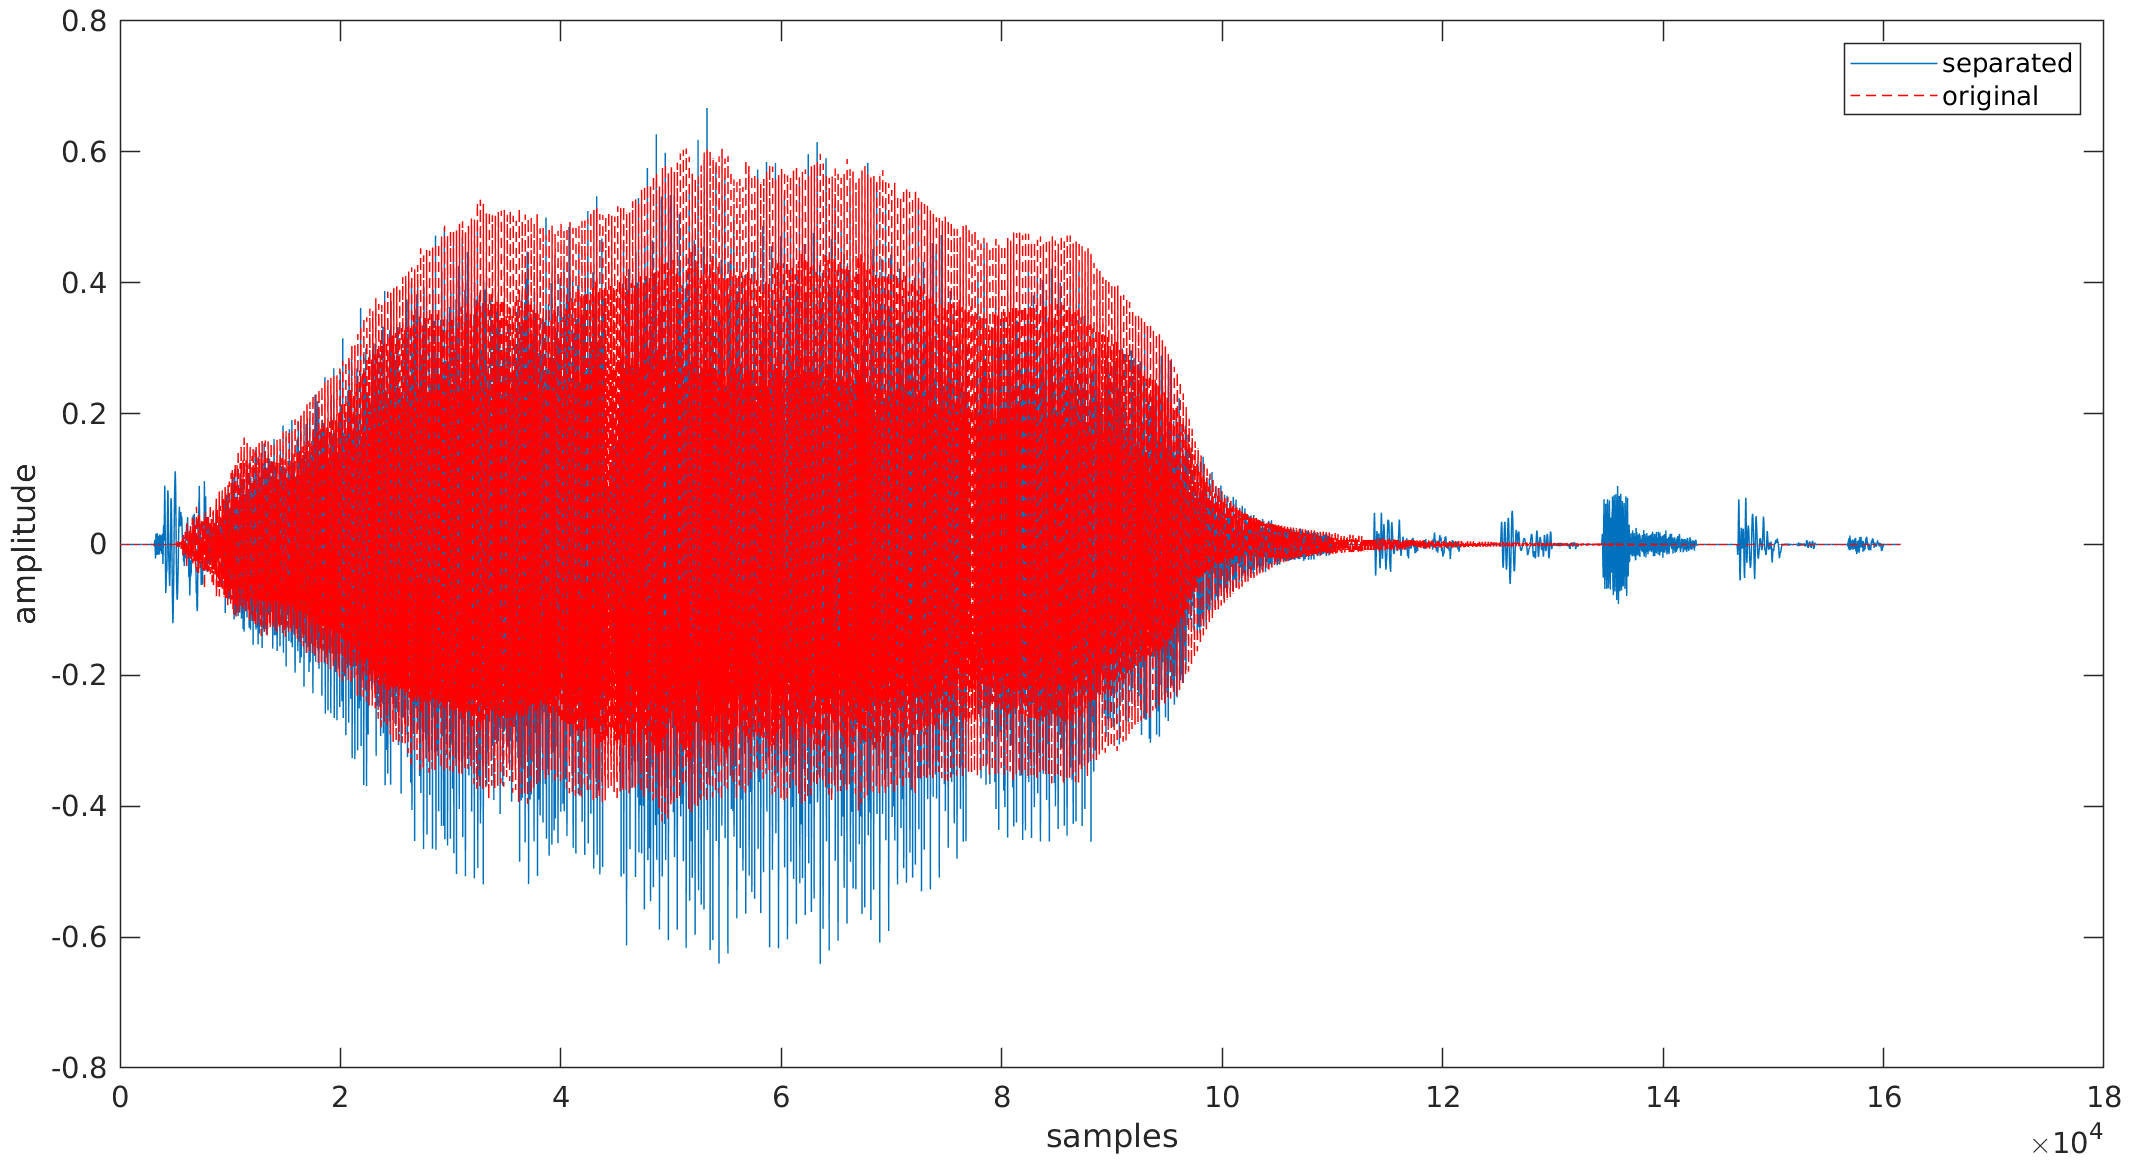
\includegraphics[width=12cm]{../images/harm_driedger_cmp.png} }}
	\caption{Harmonic separation results, time-domain waveform}
	\label{fig:harmwaveformresult}
\end{figure}

\begin{figure}[ht]
	\centering
	\subfloat[Original mixed waveform]{{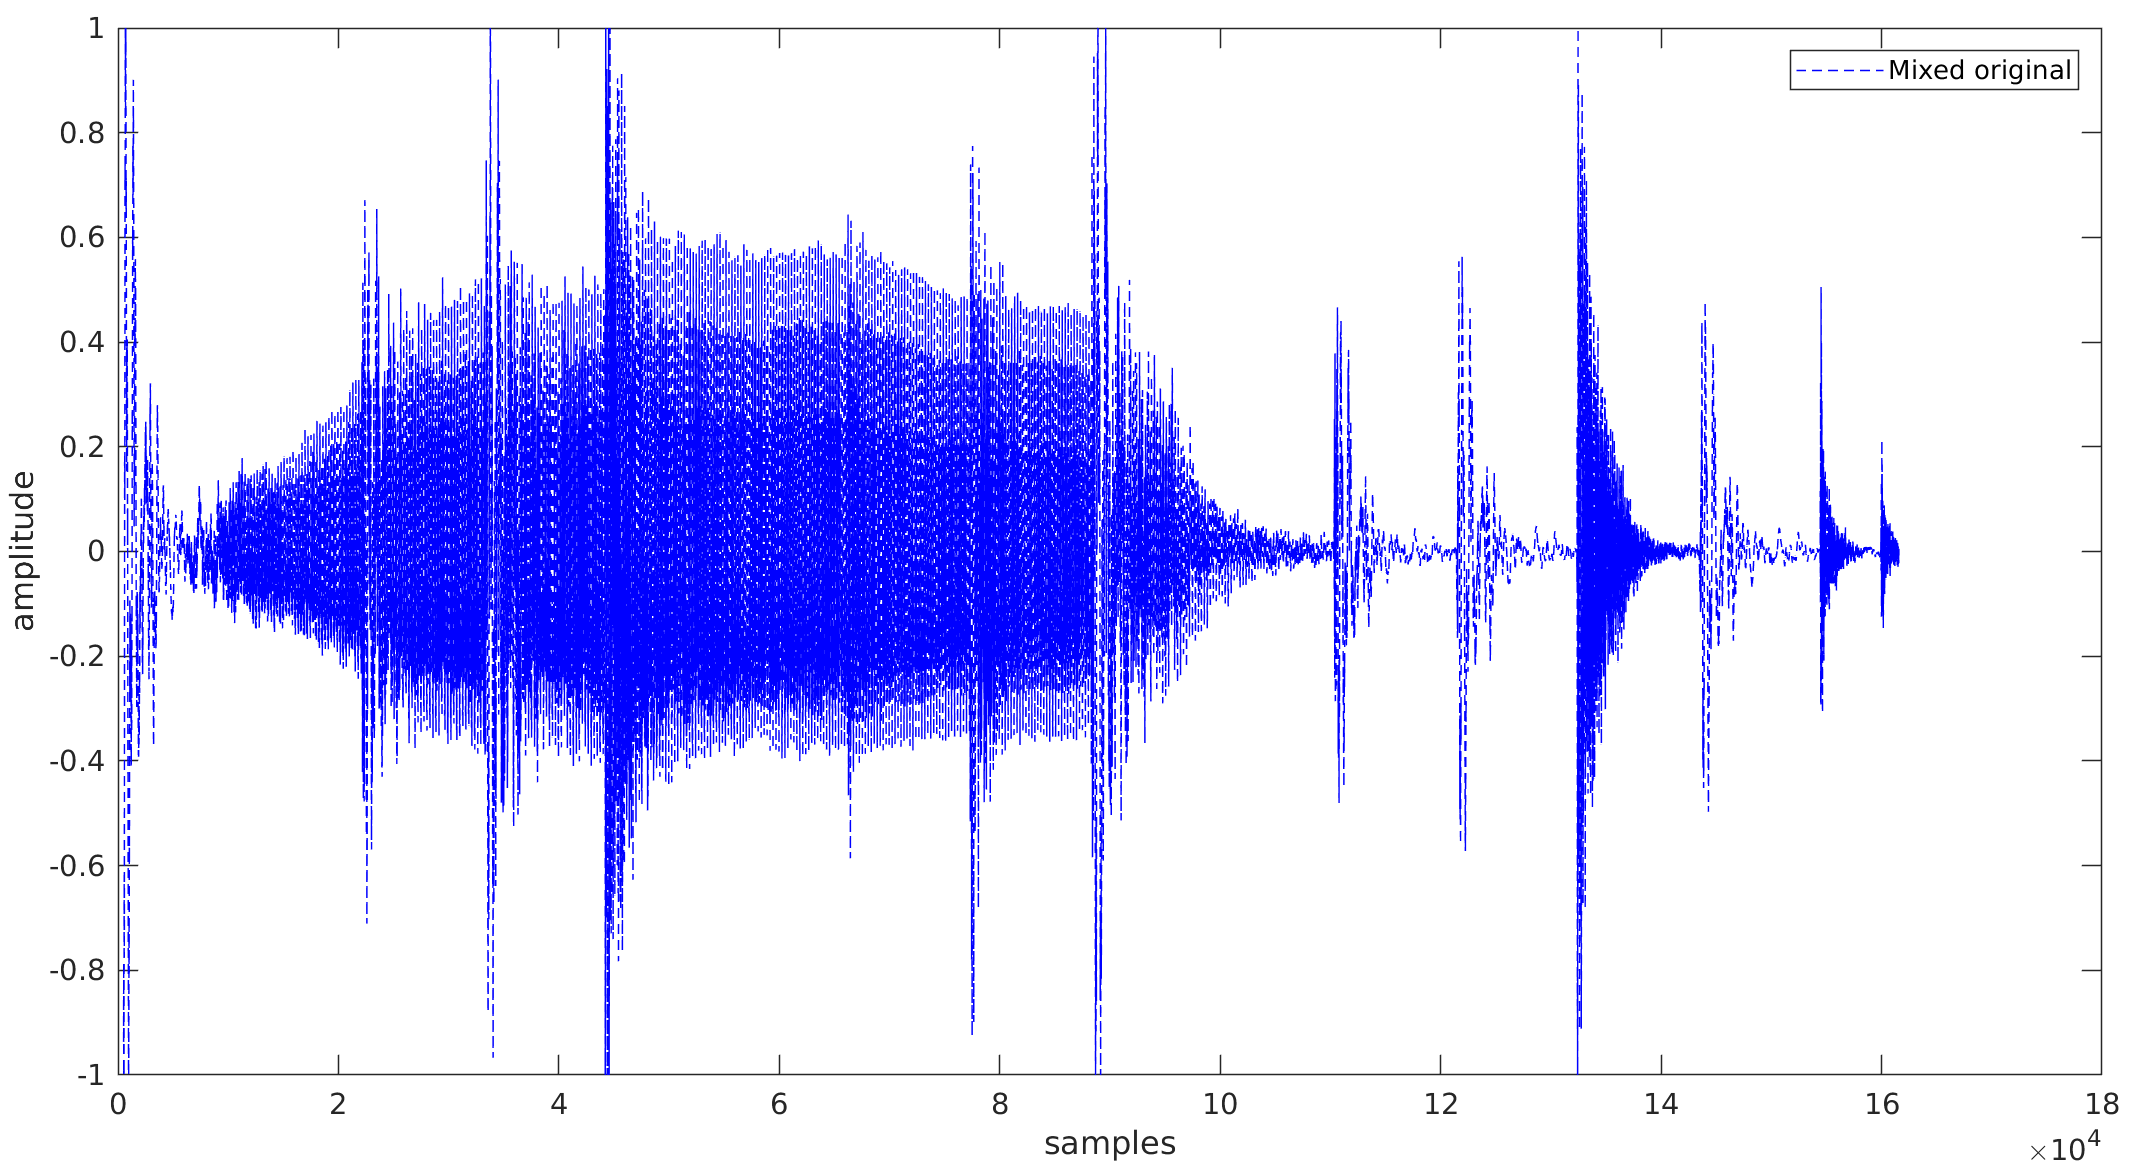
\includegraphics[width=12cm]{../images/waveform_realtime_orig.png} }}
	\\
	\subfloat[Percussive separated vs. original, soft mask]{{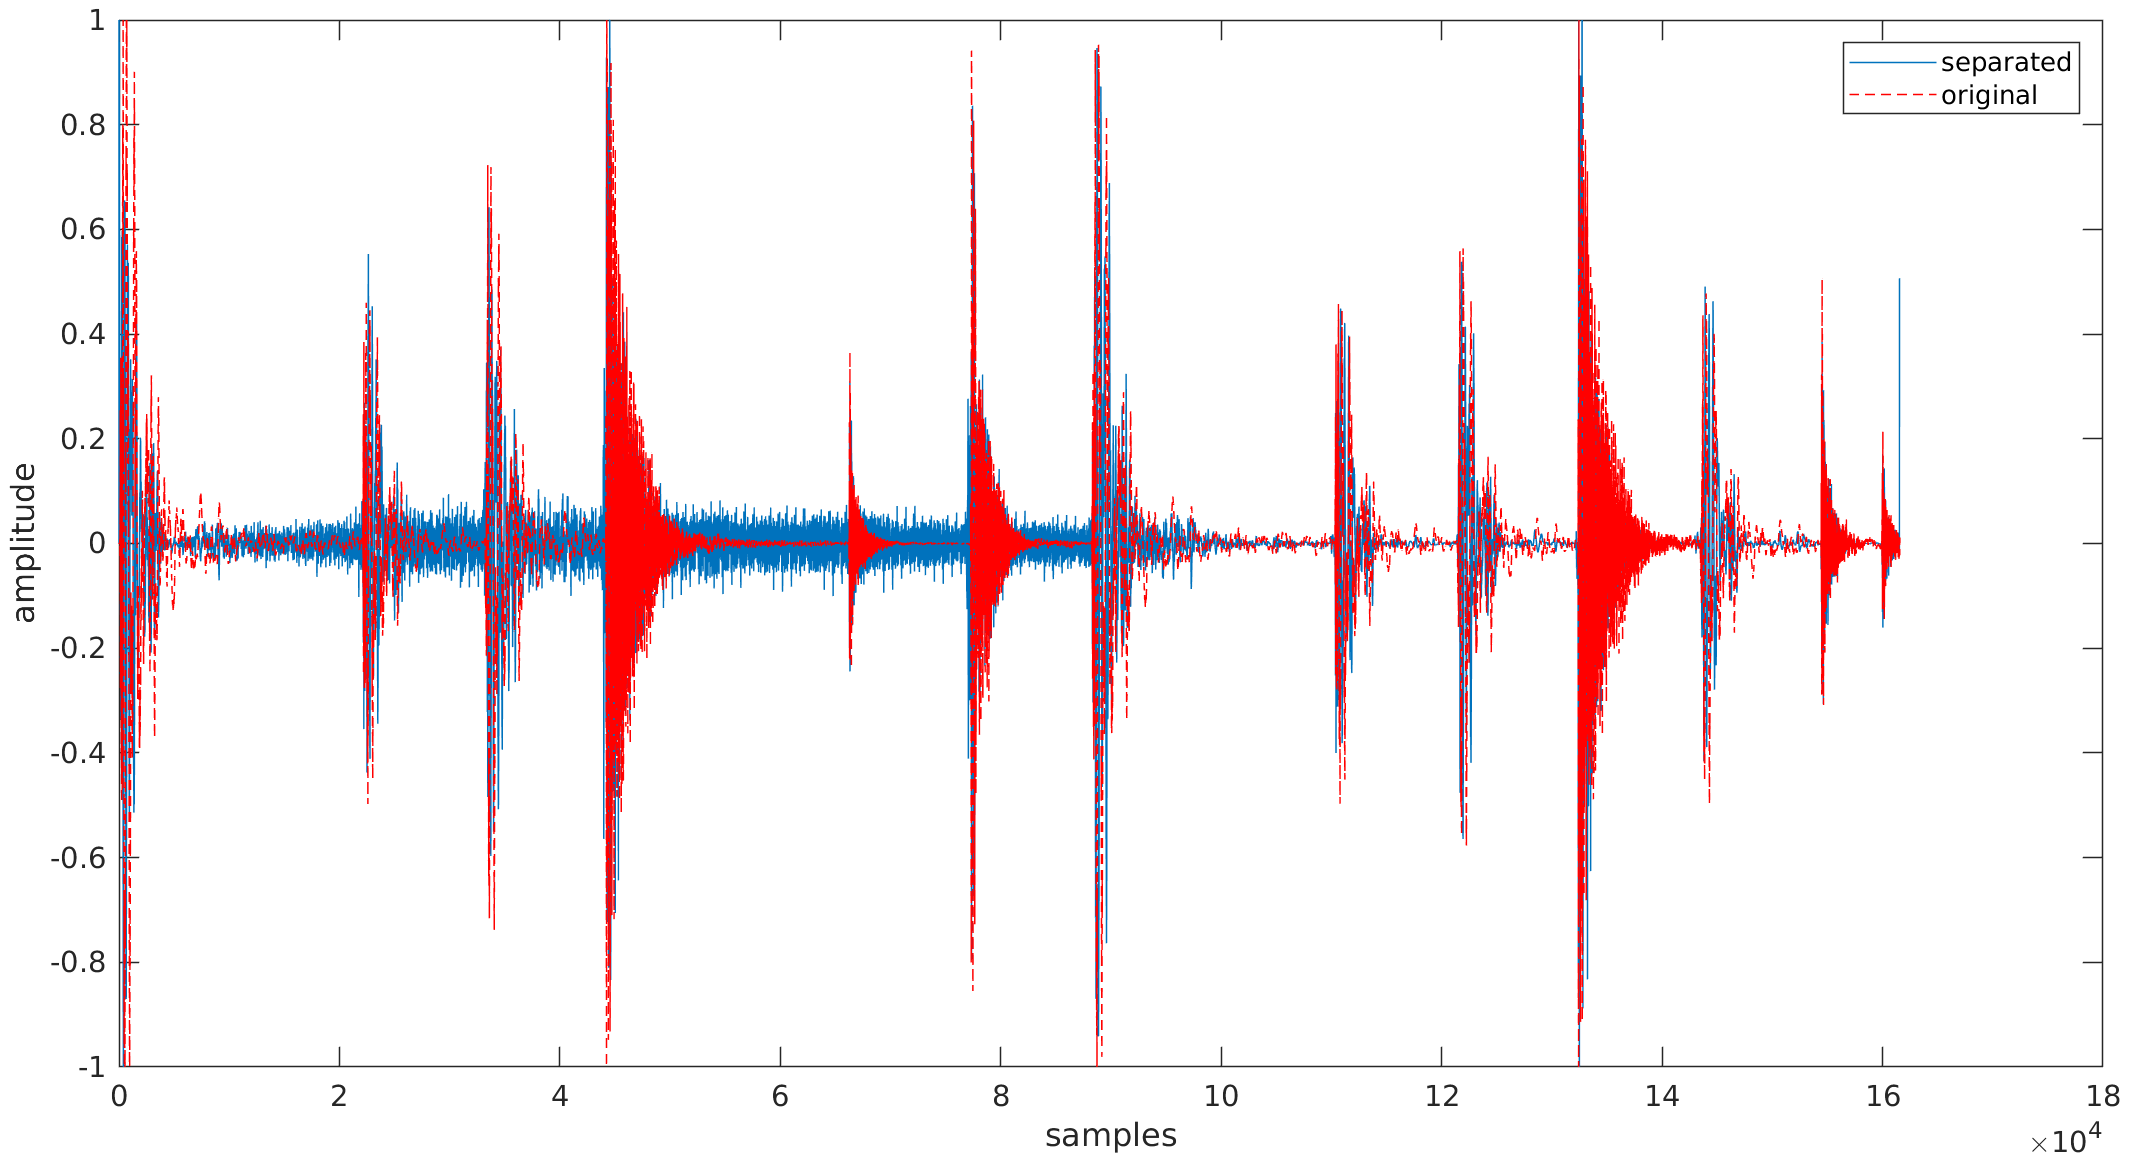
\includegraphics[width=12cm]{../images/perc_fitzgerald_cmp.png} }}
	\\
	\subfloat[Percussive separated vs. original, binary mask]{{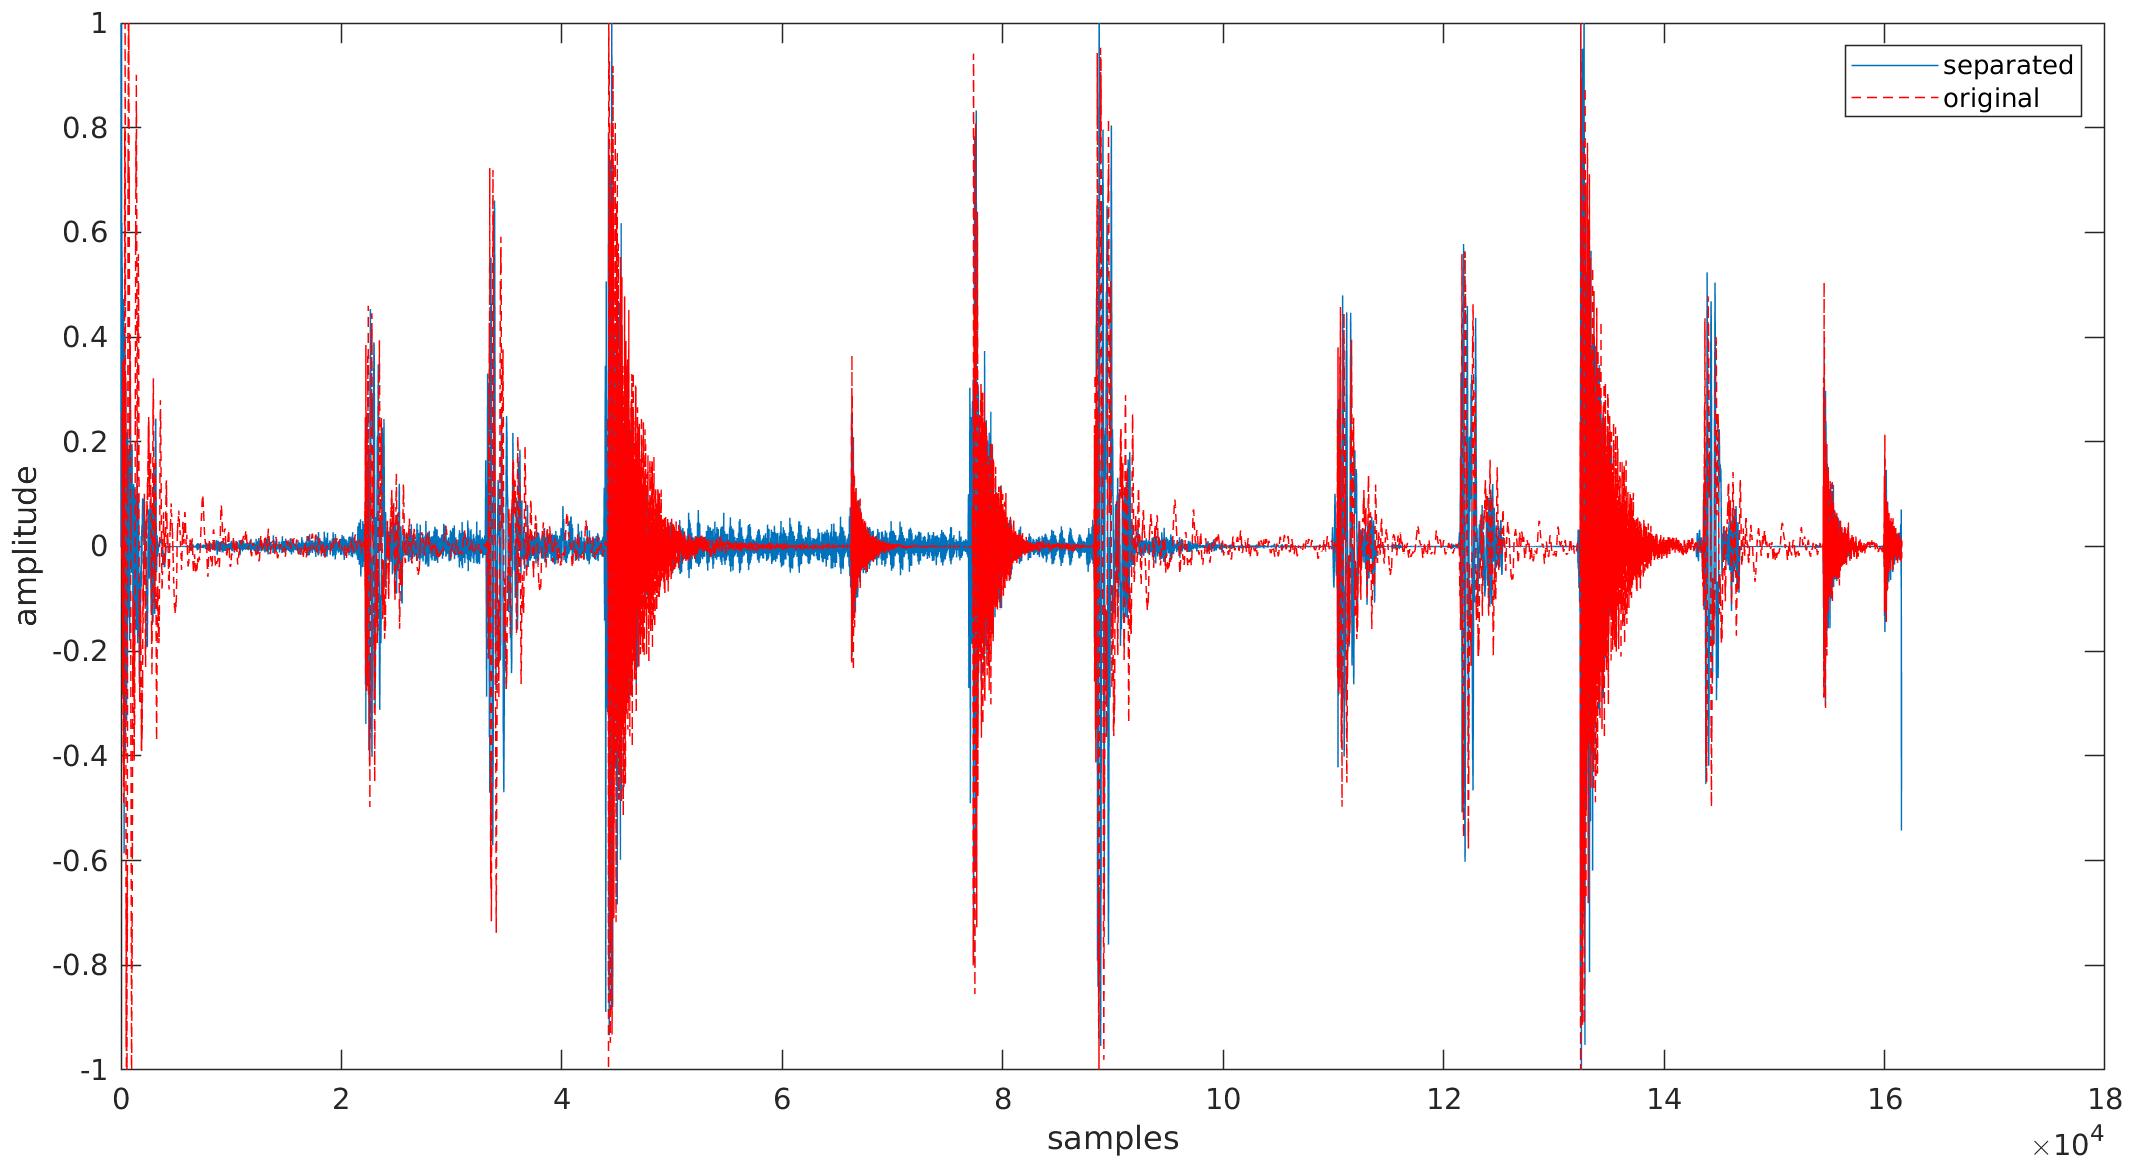
\includegraphics[width=12cm]{../images/perc_driedger_cmp.png} }}
	\caption{Percussive separation results, time-domain waveform}
	\label{fig:percwaveformresult}
\end{figure}

\begin{figure}[ht]
	\vspace*{-0.5cm}
	\centering
	\subfloat[Harmonic original spectrogram]{{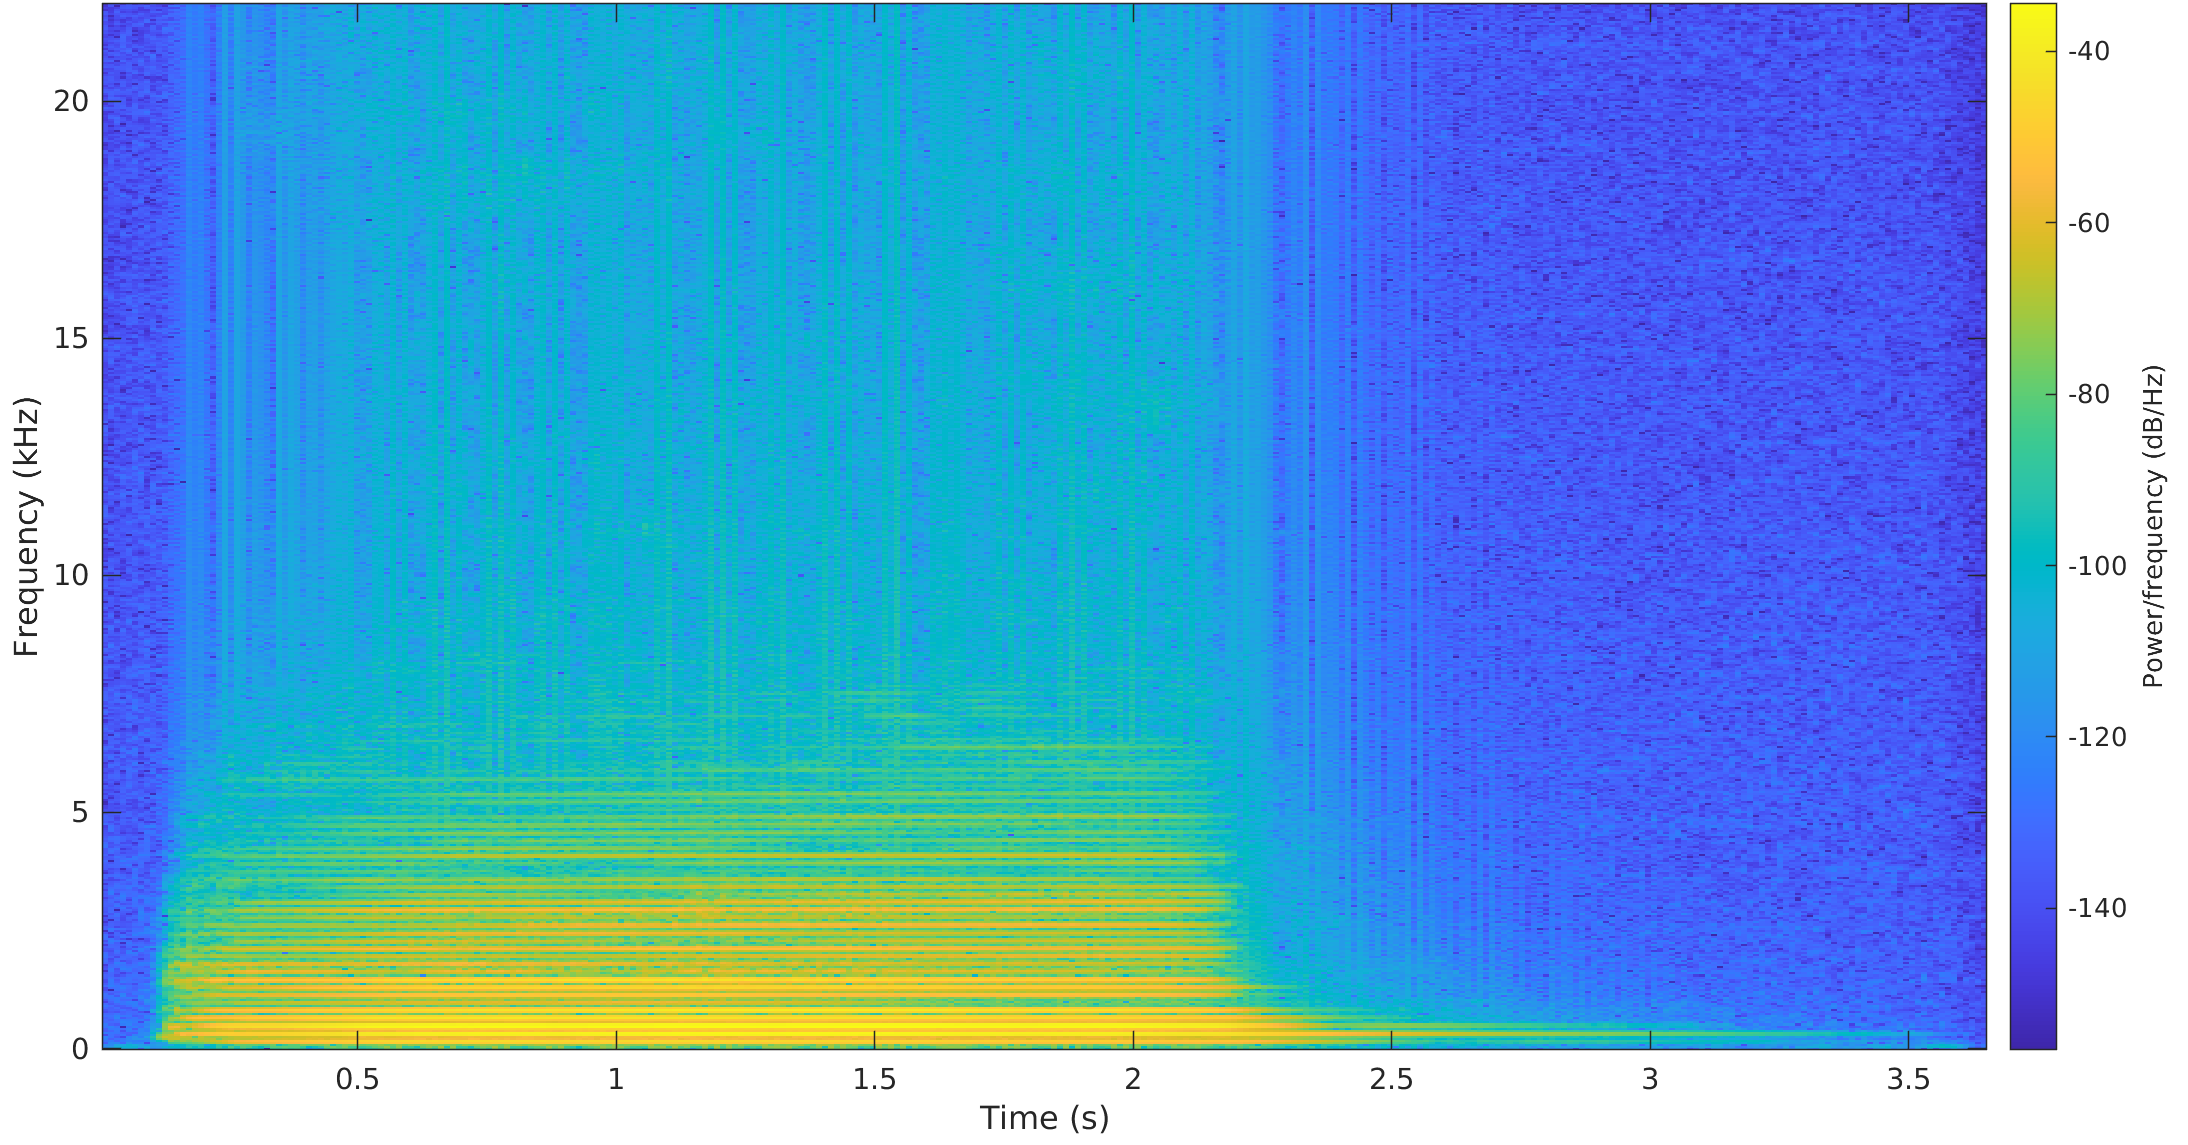
\includegraphics[width=12cm]{../images/violaspecgram.png} }}
	\\
	\subfloat[Harmonic separated, soft mask]{{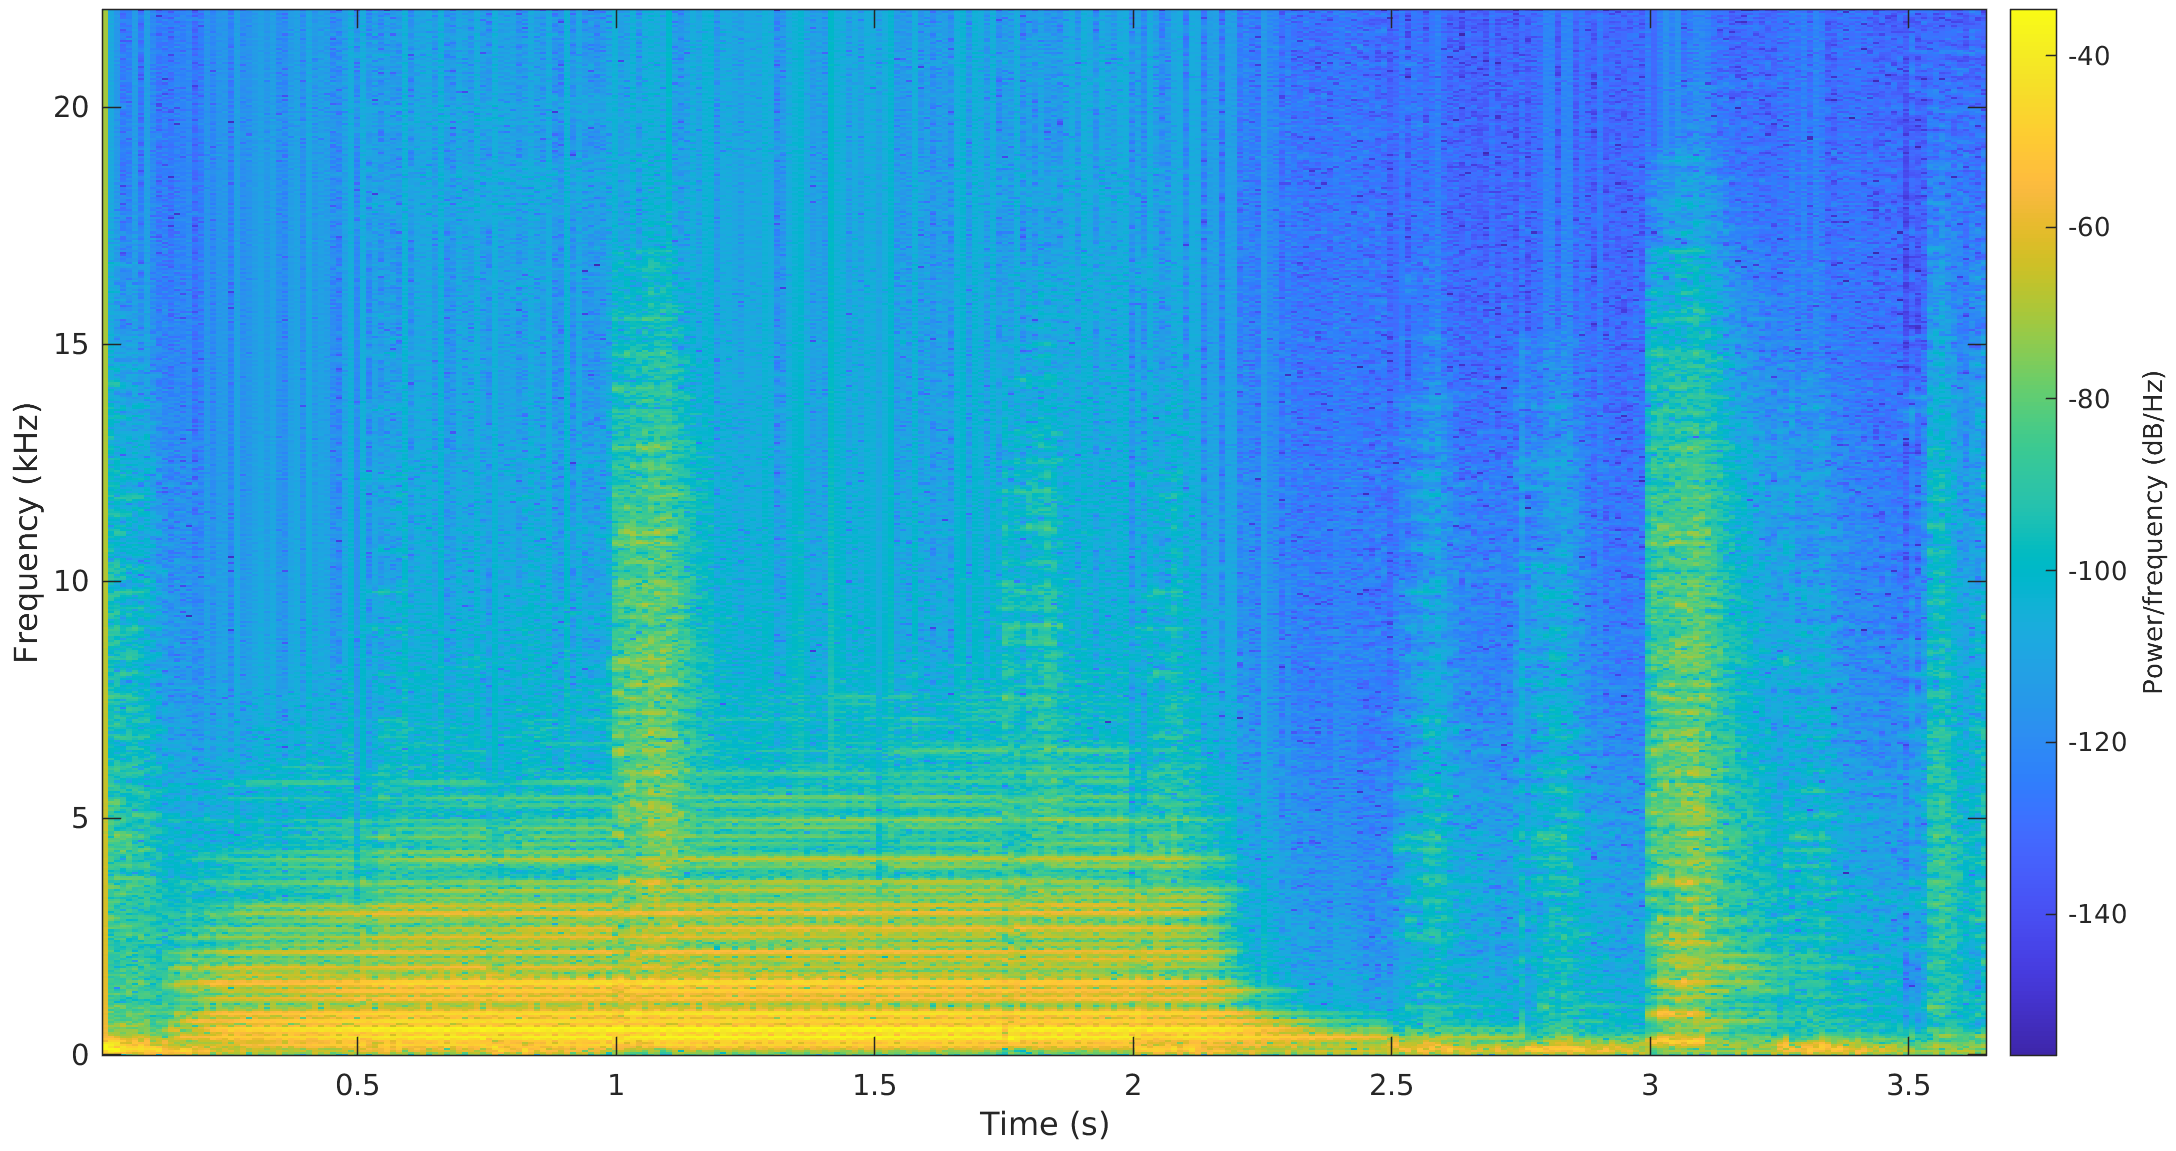
\includegraphics[width=12cm]{../images/harm_soft.png} }}
	\\
	\subfloat[Harmonic separated, binary mask]{{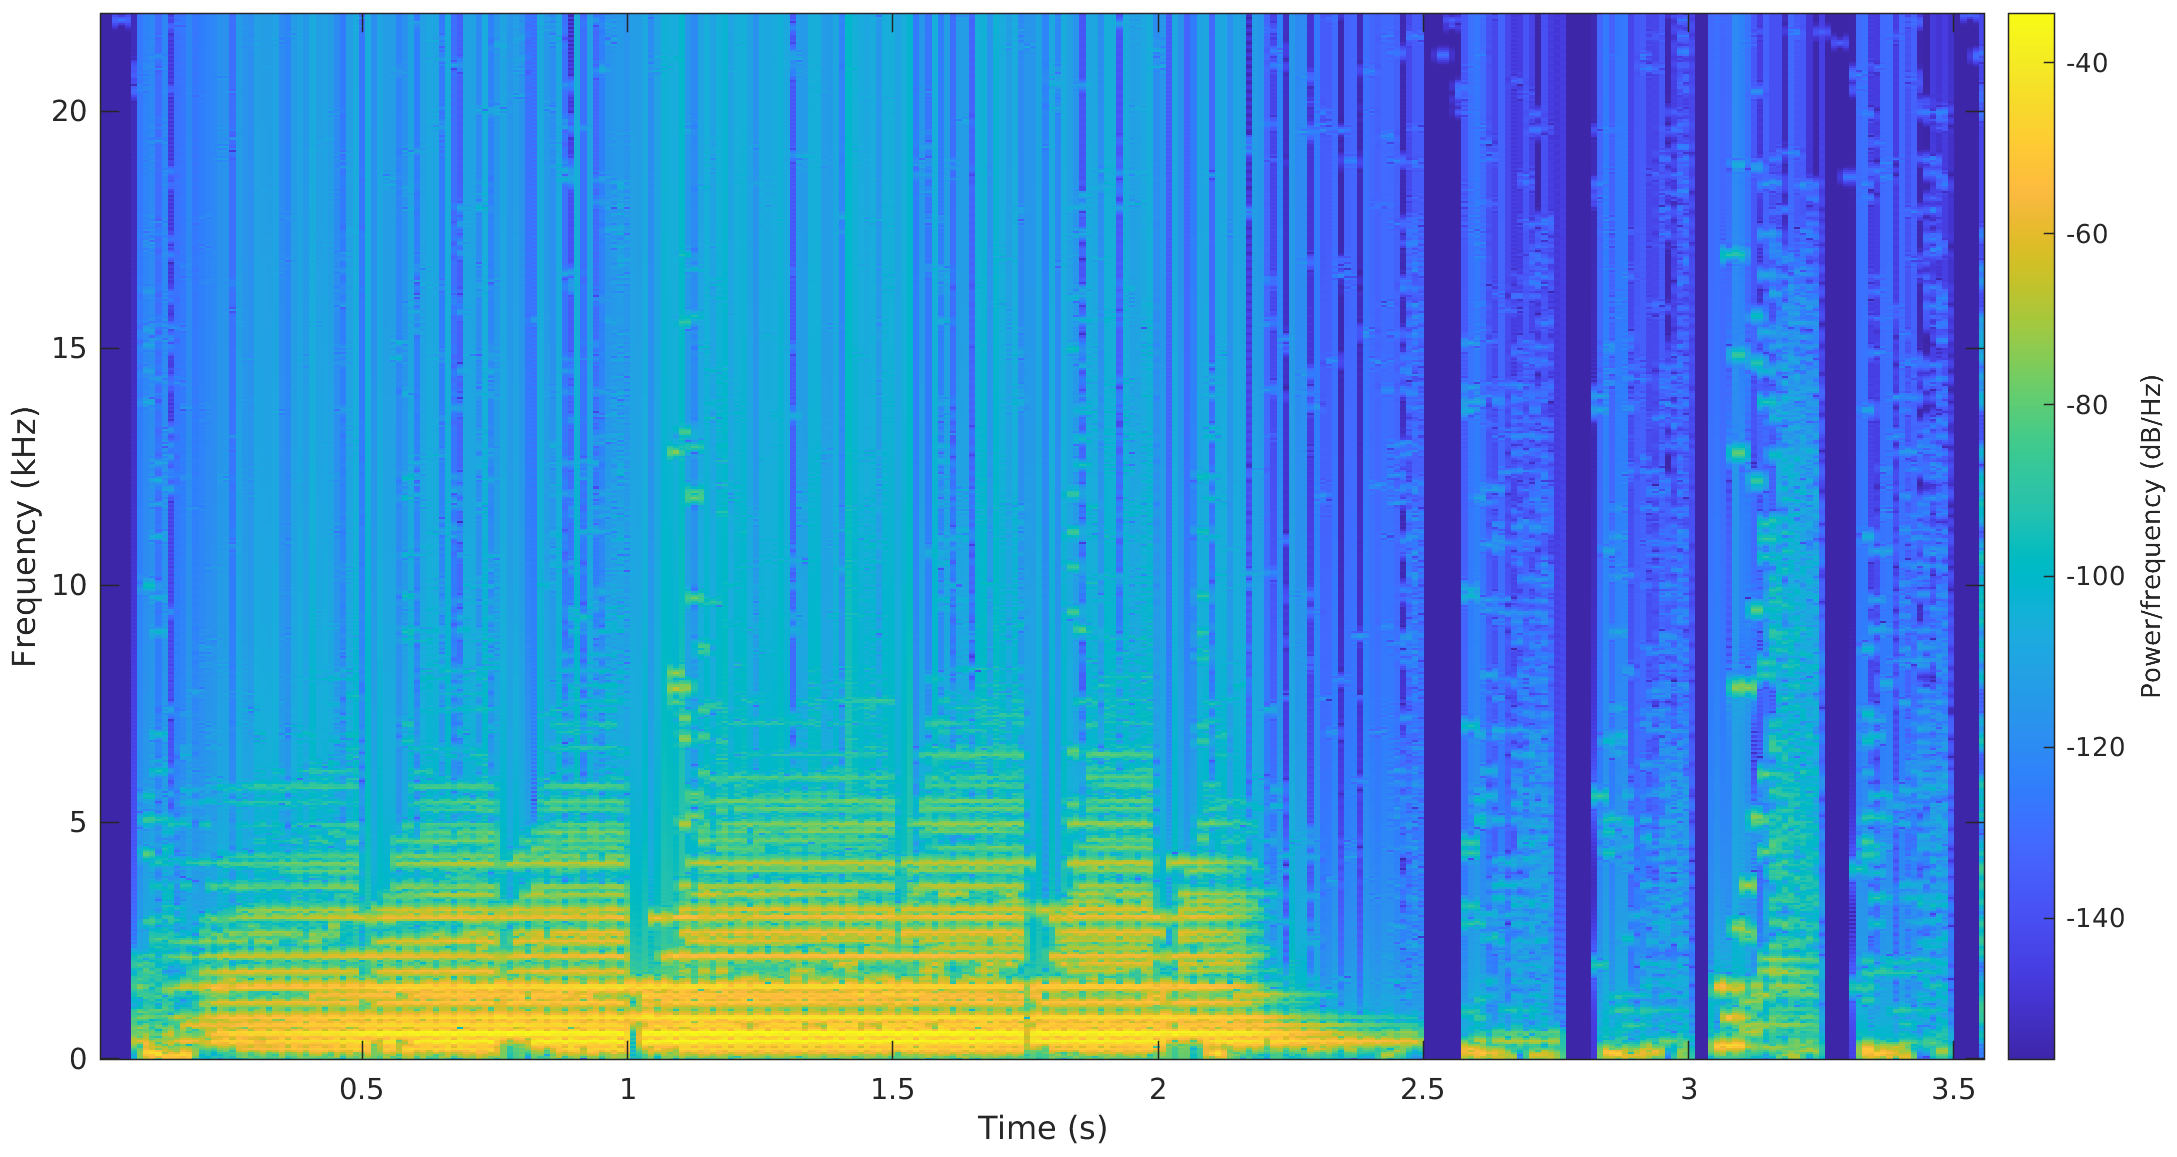
\includegraphics[width=12cm]{../images/harm_binary.png} }}
	\caption{Harmonic separation result, spectrogram}
	\label{fig:harmspecresult}
\end{figure}

\begin{figure}[ht]
	\vspace*{-0.5cm}
	\centering
	\subfloat[Percussive original spectrogram]{{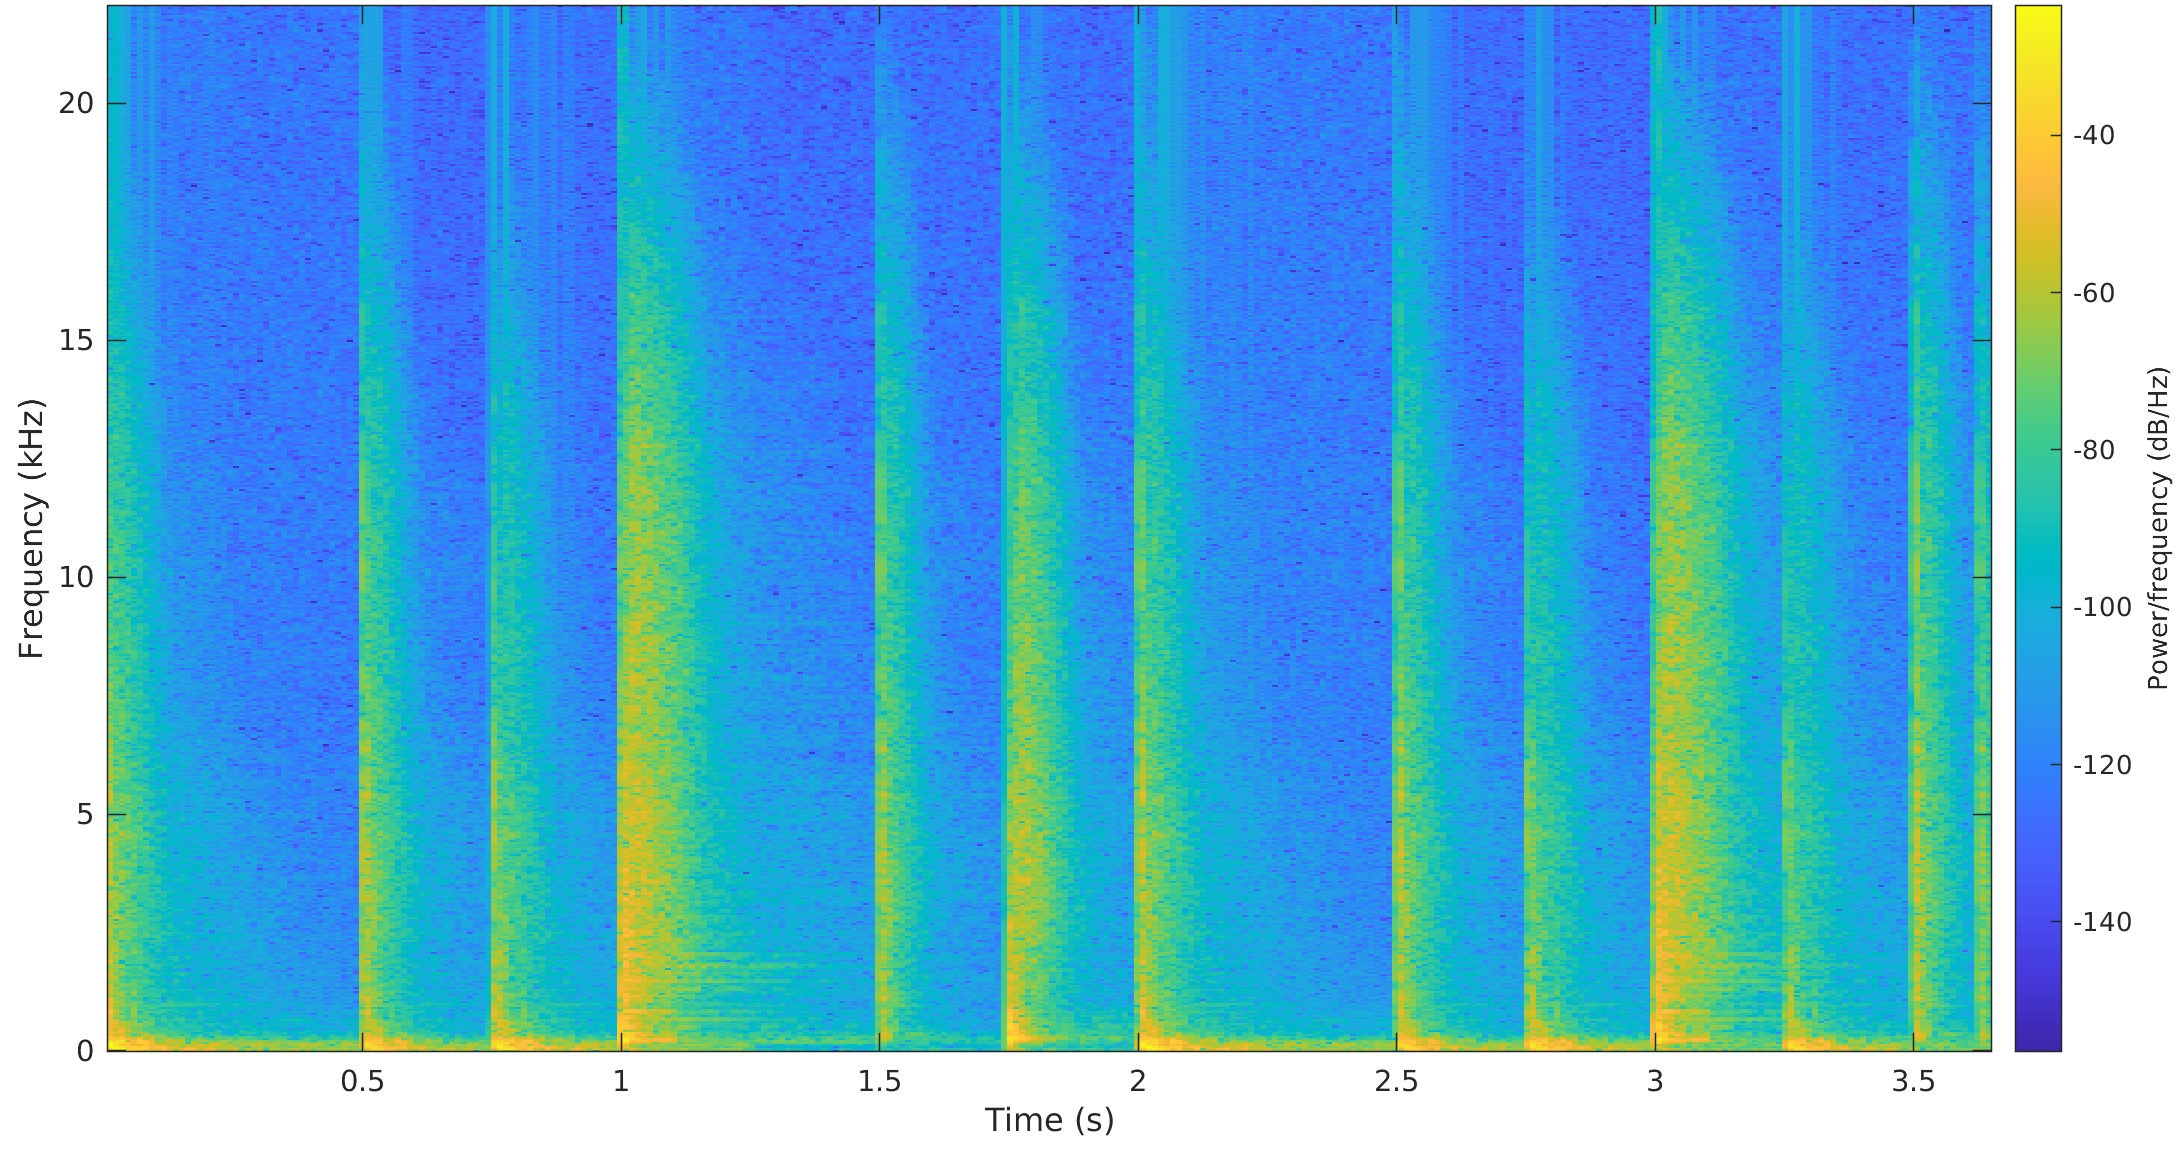
\includegraphics[width=12cm]{../images/drumspecgram.png} }}
	\\
	\subfloat[Percussive separated, soft mask]{{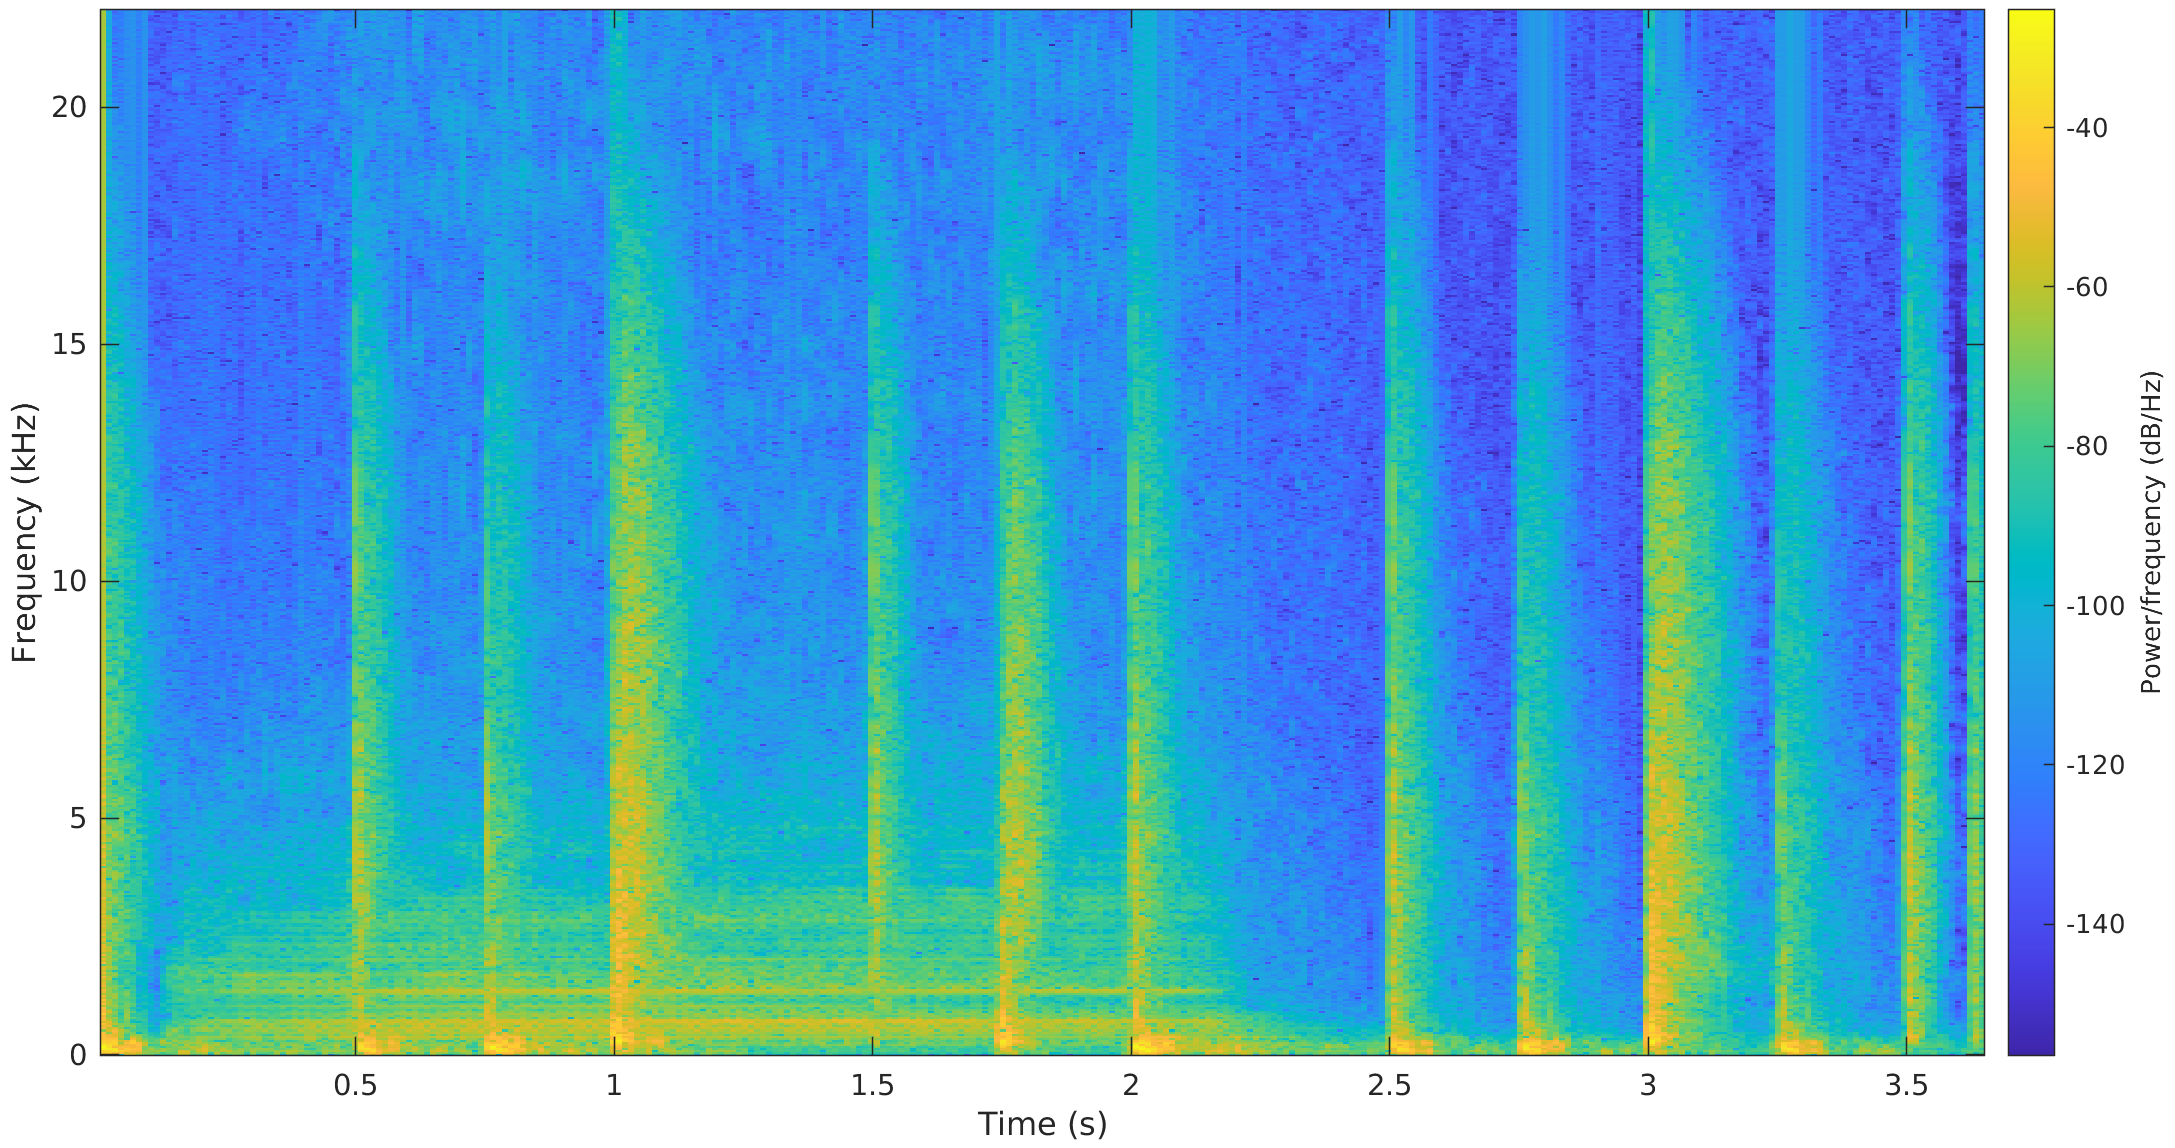
\includegraphics[width=12cm]{../images/perc_soft.png} }}
	\\
	\subfloat[Percussive separated, binary mask]{{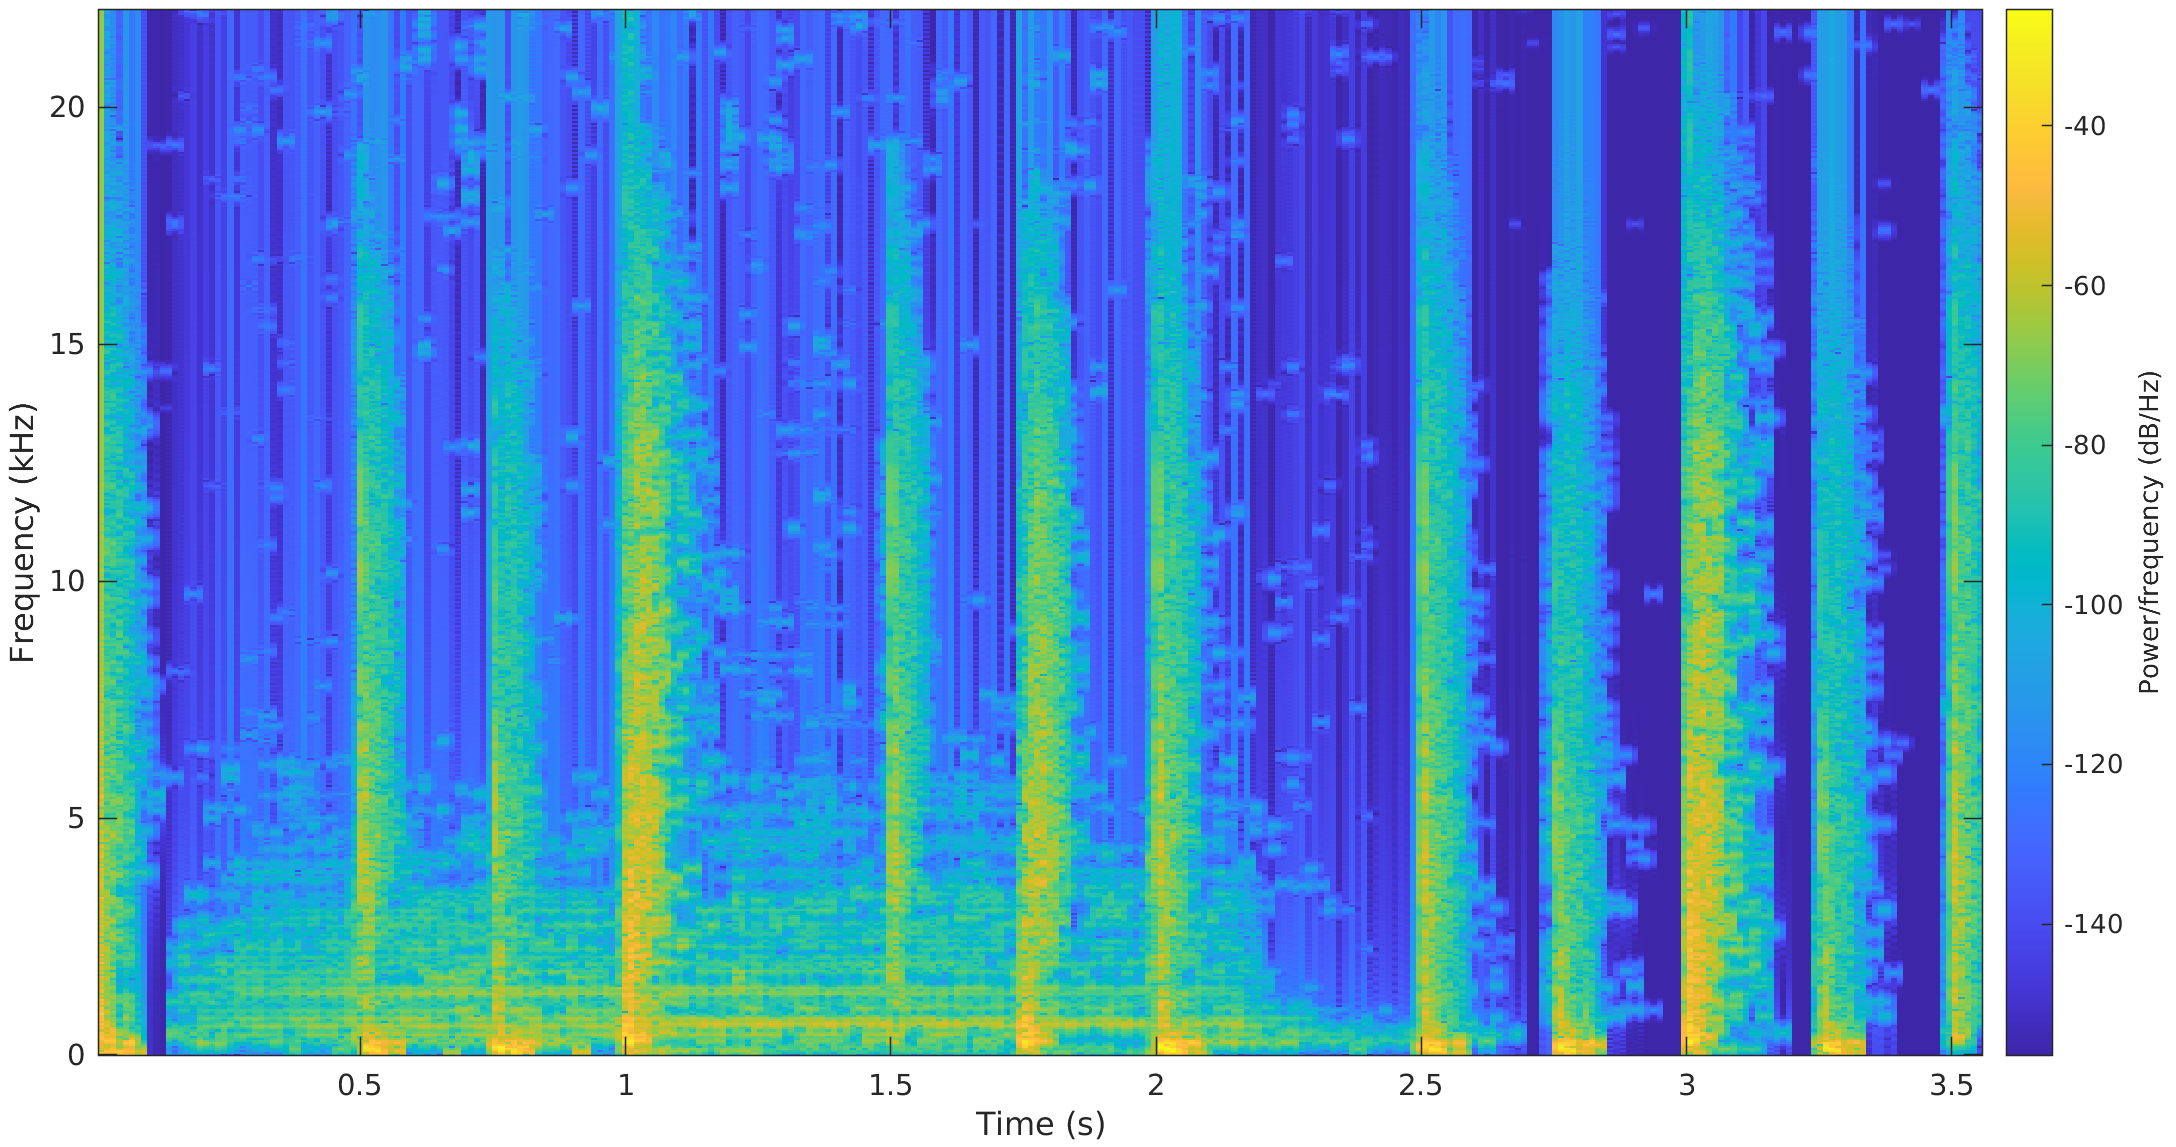
\includegraphics[width=12cm]{../images/perc_binary.png} }}
	\caption{Percussive separation result, spectrogram}
	\label{fig:percspecresult}
\end{figure}

\begin{listing}[h]
\setlength\partopsep{-\topsep}
\begin{inputminted}[linenos,breaklines,frame=single,]{matlab}{../matlab/HPSS.m}
\end{inputminted}
\caption{Full implementation of HPSS}
\label{code:fullimpl}
\end{listing}

\vfill
\clearpage %force a page break

\subsection{STFT details -- window, overlap, and COLA compliance}

In section 2 a high-level overview of the STFT was given, and some description of STFT windowing and overlapping. The selection of window and overlap parameters in a real-world HPSS implementation is not obvious, and the two papers do not mention details. Fortunately, there is a Mathworks article \cite{god} with a reference implementation of median-filtering HPSS. The STFT parameters used are a square-root von Hann window with $L = 1024$, \textit{overlap} = $512$, \textit{NFFT} = $2048$. Without using these parameters in my implementation, the pitch of the viola in the resulting harmonic separation was incorrect.\\

The window and overlap were also verified to be COLA-compliant with the ``iscola'' function in MATLAB \cite{cola}. The function ``ensures that the inverse short-time Fourier transform results in perfect reconstruction for nonmodified spectra.'' The diagram of inverse signal reconstruction included in the ``iscola'' documentation is a perfect introduction to the properties of the STFT that I will be using to adapt HPSS to work in real-time in the next section:

\begin{figure}[ht]
	\centering
	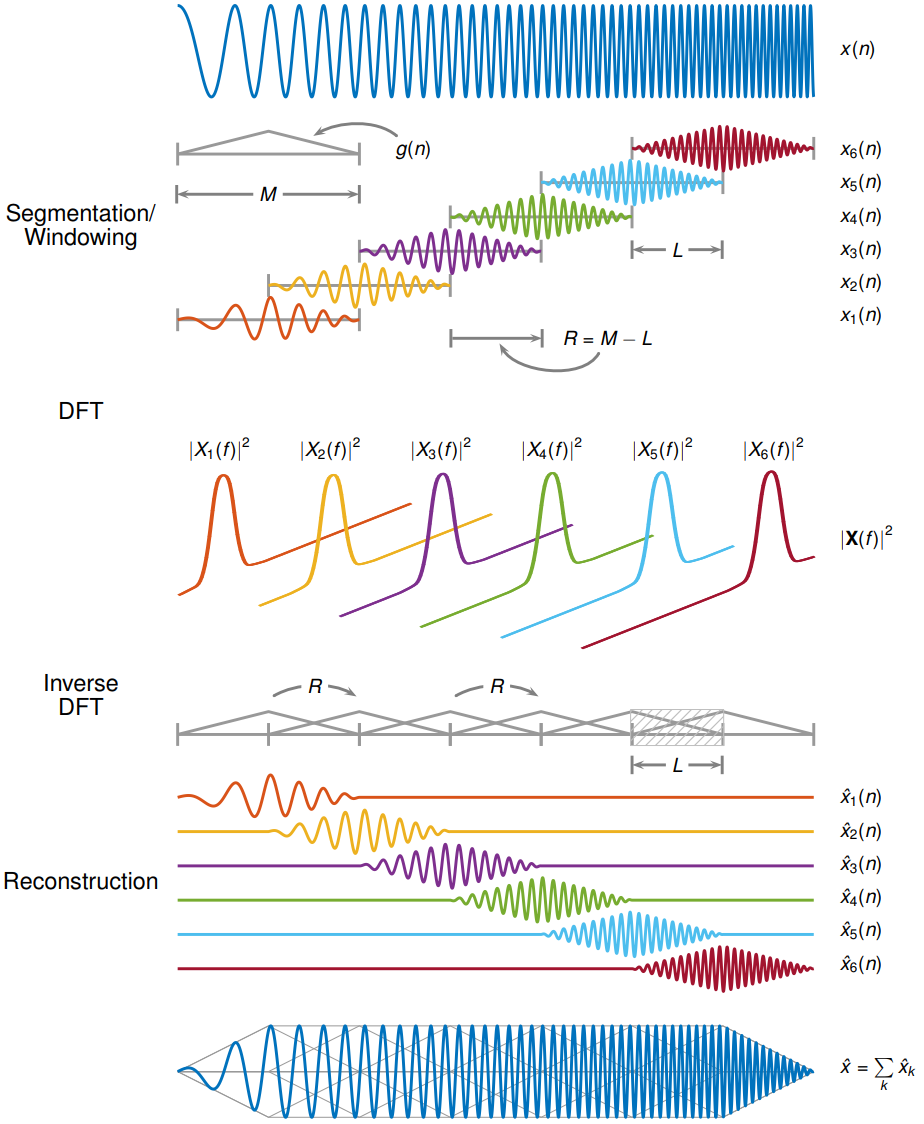
\includegraphics[width=12cm]{../images/iscola0111.png}
	\caption{STFT/ISTFT signal reconstruction}
	\label{fig:cola}
\end{figure}

\vfill
\clearpage %force a page break

\section{Real-time HPSS}

The final version of the algorithm should take a real-time input stream and emit real-time harmonic-percussive separated output streams. Let's begin by considering that the STFT is already itself a chunked processing of the input signal. It might be easier to visualize it with a sketch in Figure~\ref{fig:stftdiag}, based on the STFT/ISTFT MATLAB implementations in \cite{stftchunks1}.

\begin{figure}[ht]
	\centering
	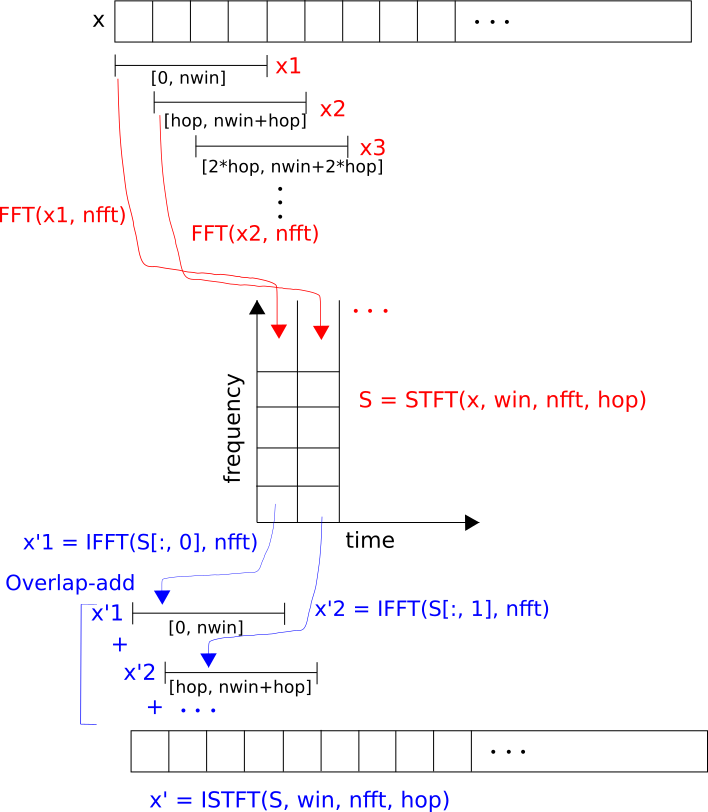
\includegraphics[width=12cm]{../images/stft_diagram.png}
	\caption{STFT and ISTFT diagram}
	\label{fig:stftdiag}
\end{figure}

The STFT matrix consists of frames/columns that are the FFT of time-overlapping blocks of the input signal $x$. In the ISTFT, the IFFTs are overlap-added. This means the IFFT of the current frame/column shares \textit{hop} overlap with the IFFT of the frame before it. We can see it in the above diagram in blue. The important implication here is that after processing the current frame in the STFT, the first \textit{hop} samples of the ISTFT output will be overlap-added with the previous \textit{hop} samples, and will not be overlap-added to any future samples -- they are final.\\

The real-time HPSS implementation would be embedded inside an STFT ``round-trip'' algorithm. An $nwin$-sized frame would have the FFT applied to create the newest frame of the STFT. The STFT so far can be median-filtered to create the masks $M_{\text{h}}, M_{\text{p}}$. The masks can be applied to the previous FFT to create $\text{H}_{\text{FFT}}$ and $\text{P}_{\text{FFT}}$. The IFFT is taken, overlap-adding the result with the tail \textit{hop} samples of the previous ISTFT result. This resulting first \textit{hop} of the sum represents fully separated chunks of harmonic and percussive audio. This is illustrated in Figure~\ref{fig:rthpssdiag}:

\begin{figure}[ht]
	\centering
	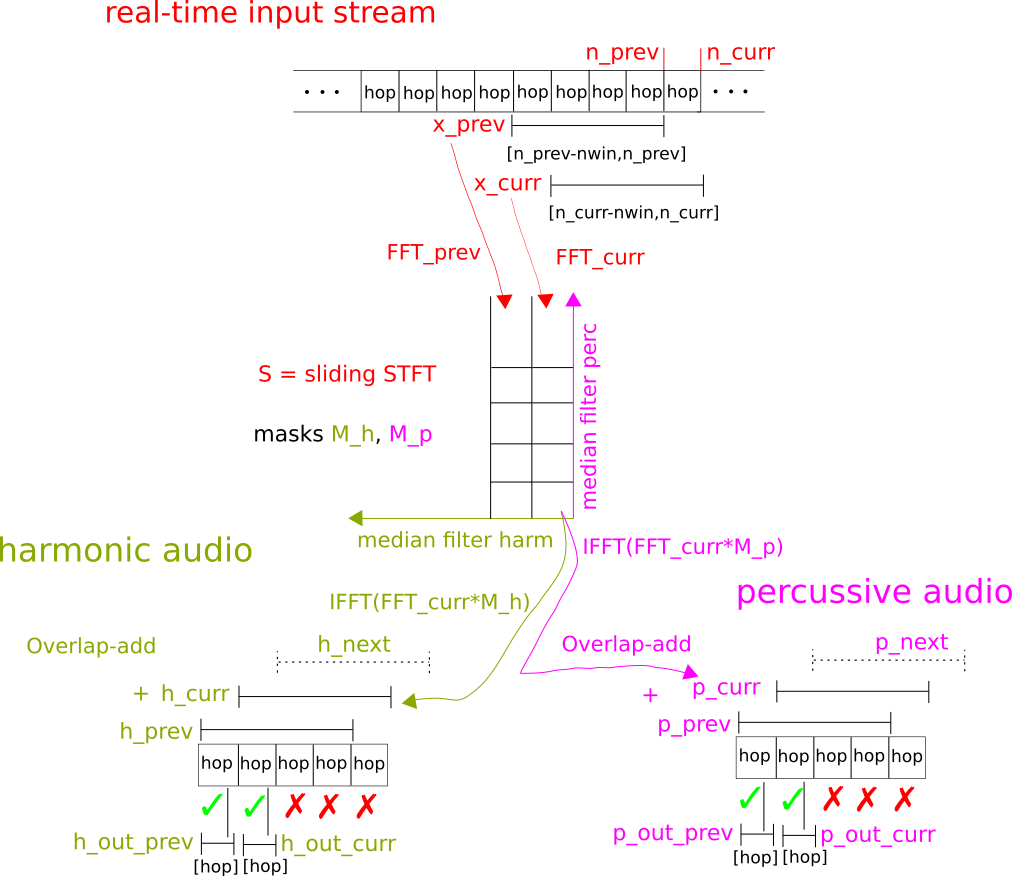
\includegraphics[width=16cm]{../images/rt_hpss_diagram.png}
	\caption{Real-time HPSS system block diagram}
	\label{fig:rthpssdiag}
\end{figure}

It might help to present a pseudocode/prose description of the above block diagram. Using input buffer \textit{x[1024]}, output buffers \textit{h[1024]}, \textit{p[1024]}, \textit{hop = 512}:
\begin{tight_enumerate}
	\item Receive a chunk of 512 samples, \textit{x\_current}, from input stream
	\item Append to right of buffer \textit{x}: \textit{x = x[512:1024] + x\_current}
	\item Calculate FFT of \textit{x} and append to sliding STFT matrix
	\item Calculate harmonic, percussive masks with median filtering
	\item Apply IFFT to masked FFT to get \textit{h\_current}, \textit{p\_current}
	\item Weighted overlap-add: \textit{h = h + h\_current}, \textit{p = p + p\_current}
	\item \textit{h[0:512]}, \textit{p[0:512]} represent the correct, final harmonic/percussive separation of \textit{x\_current}
	\item Shift h, p left: \textit{h = h[512:1024] + zeros(512)}, \textit{p = p[512:1024] + zeros(512)} for future weighted overlap-add
	\item  Repeat
\end{tight_enumerate}

A detail to discuss is the size of the sliding STFT. In the offline HPSS, the STFT of the entire waveform is taken. In real-time HPSS, the STFT matrix is built and maintained in a loop while processing consecutive chunks of the input stream. The vertical median filter operates in the frequency axis, i.e. on each FFT result/STFT column. Therefore, at each iteration of the input processing loop, once the FFT is taken, there is enough information to do a full $l_{\text{perc}}$ vertical median filter. On the other hand, the horizontal median filter operates on the time axis, which presents a problem when considering real-time vs. offline behavior.\\

The horizontal median filter has length $l_{\text{harm}}$ as 17 in the original 2010 variant, and 200ms in samples ($\approx$ 12) in the 2014 paper. Referring back to the MATLAB ``movmedian'' documentation \cite{movmedian}, the moving median is computed for a window of $k$ (i.e. $l_{\text{harm}}$ in this case) centered at the current point, and \textbf{the window is truncated when there are not enough elements to fill it}. This means that the sliding STFT matrix only needs to maintain a history of $\frac{l_{\text{harm}}}{2}$ FFT columns. In MATLAB syntax, this could look something like:

\begin{verbatim}
STFT = zeros(nfft, ceil(lHarm/2));  % preallocate sliding stft
for ... % input loop
  FFT_current = fft(x); % fft of current input frame
  STFT = STFT(:, 2:size(STFT, 2)); % remove oldest stft frame 
  STFT(:, size(STFT, 2)+1) = FFT_current; % append latest FFT
end % end loop
\end{verbatim}

However, since the future $\frac{l_{\text{harm}}}{2}$ STFT columns don't exist in the real-time algorithm and are truncated from the horizontal median filter, we will get significantly worse harmonic separation performance. Given this, the binary masking 2014 HPSS will be used to compensate, as it had slightly better separation results than the soft mask 2010 variant.\\

Figure~\ref{fig:causality} is a diagram showing the causality problem of real-time HPSS, and how it would more negatively affect harmonic separation than percussive separation:

\begin{figure}[H]
	\centering
	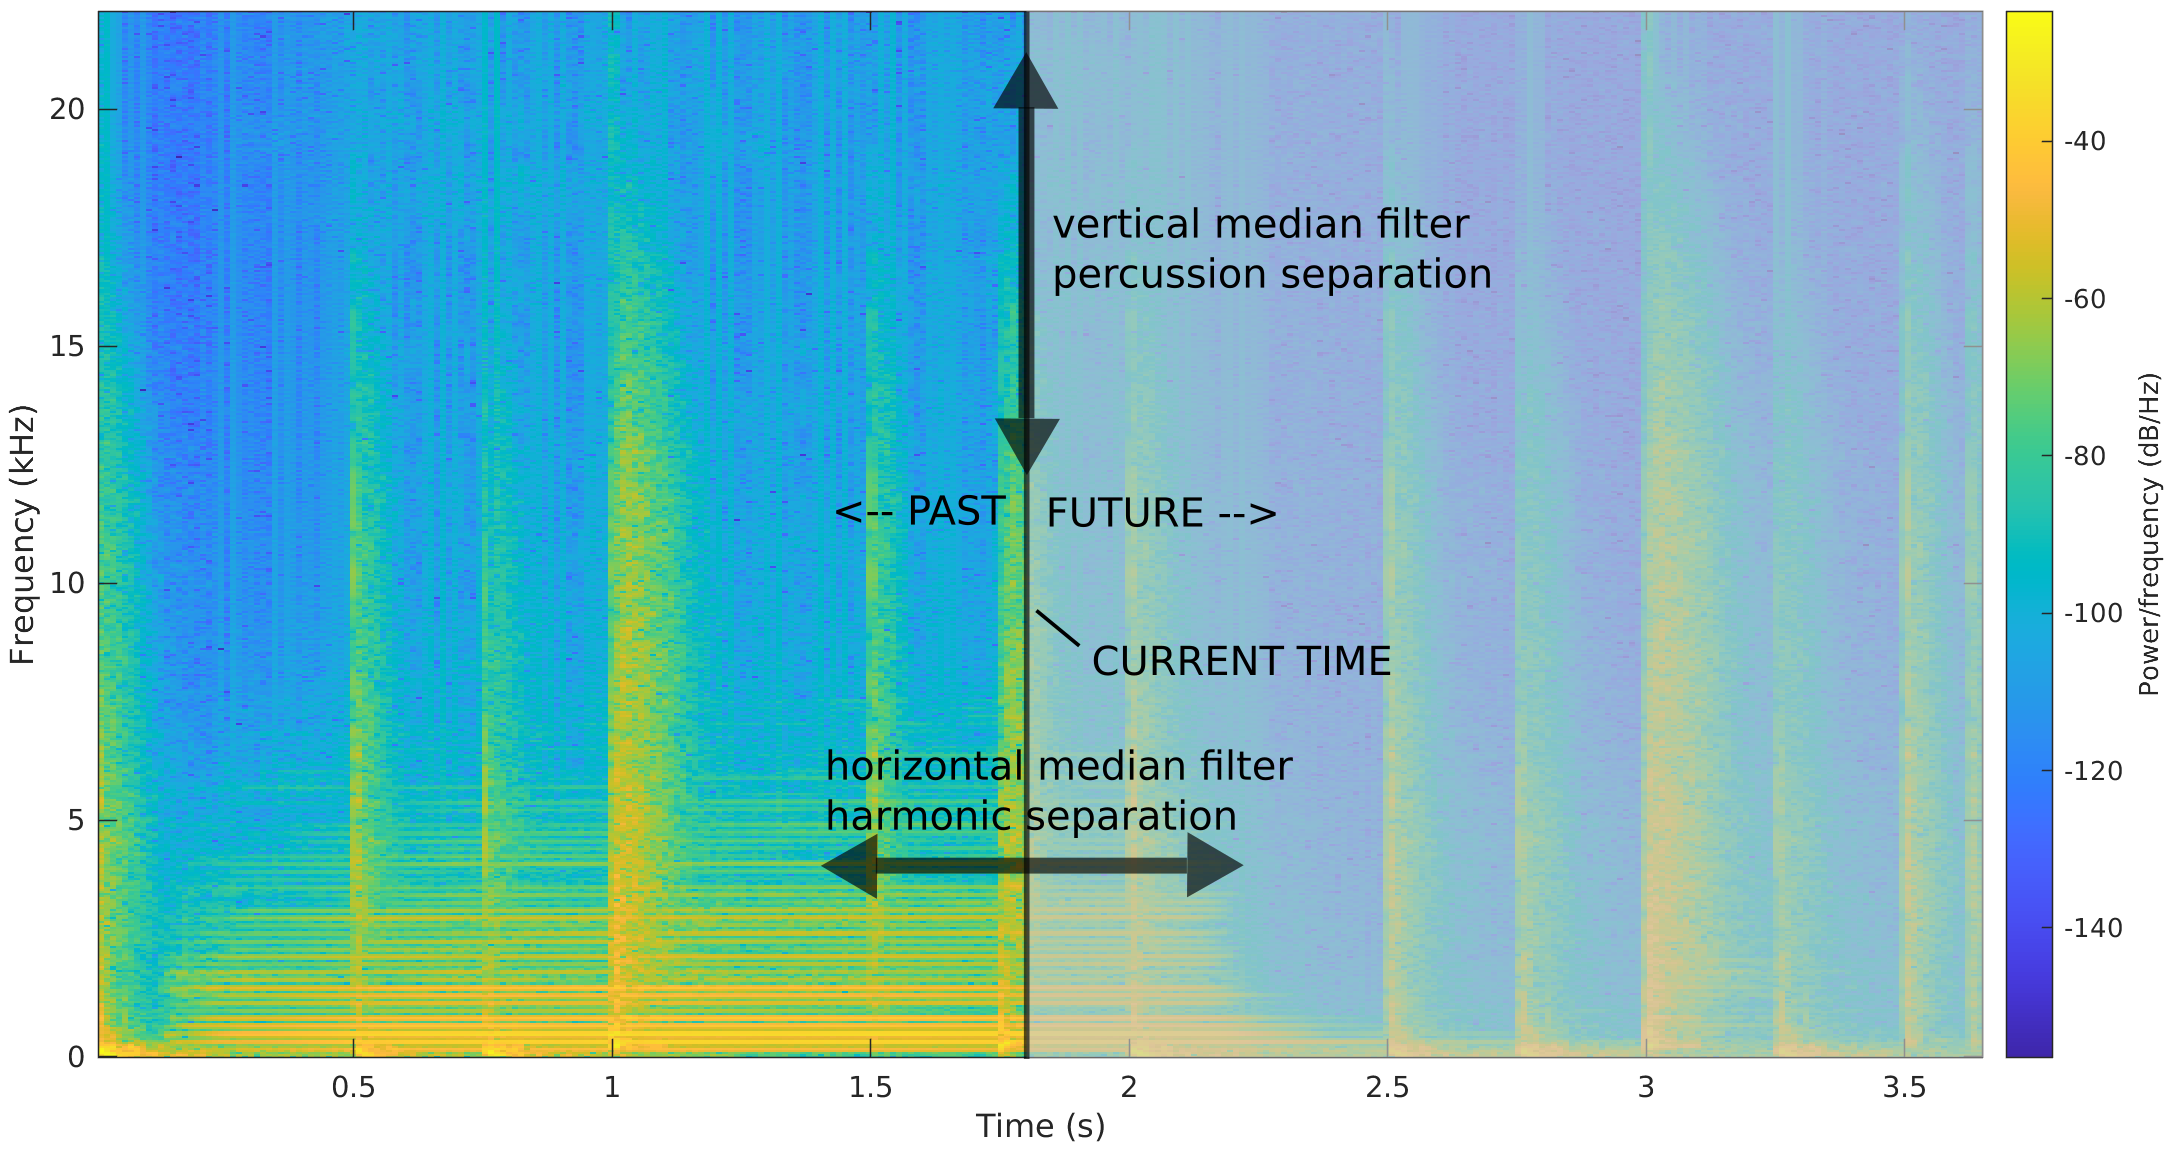
\includegraphics[width=16cm]{../images/hpss_causality.png}
	\caption{Causality of real-time HPSS}
	\label{fig:causality}
\end{figure}

No discussion of a real-time system would be complete without a latency analysis. Let's assume a case of idealized input and output streams and use real values of \textit{hop} = 512, \textit{nwin} = 1024:

\begin{enumerate}
	\item
		We receive 512 samples at a time from our real-time input stream, and accumulate them into buffer[1024], dropping the oldest 512 samples and appending the newest 512 each time
	\item
		We perform real-time HPSS on buffer[1024], generating h[512] and p[512] that can be accumulated or played on an output stream
\end{enumerate}

At a common sampling rate of 44100Hz, 512 samples represents 11.6ms. The computational time of HPSS for every 512-sized chunk needs to be low compared to 11.6ms to maintain the responsiveness of the system for human listeners \cite{realtime}. Measurements are presented with the implementations.

\subsection{MATLAB implementation and results}

The next page contains the full MATLAB implementation of real-time HPSS. The code is relatively concise, and it implements the block diagram presented in Figure~\ref{fig:rthpssdiag} in the previous section. The code is commented for clarity. The function (and file) is named ``HPSSMicrophone'' as it is a demo of HPSS performed in real-time on a microphone input stream.\\

Results will be shown and discussed on the pages following the code. To avoid the influence of microphone quality, the input and output streams have been replaced with the dsp.AudioFileWriter and dsp.AudioFileReader streams \cite{dsp1}, \cite{dsp2}, in the file ``HPSSRtWav.m'' (source available at \url{https://github.com/sevagh/Real-Time-HPSS}), which should still test the real-time aspects of the algorithm and keep most of the code looking the same.\\

As prior, the results are shown in the time-domain waveforms and spectrograms in Figures \ref{fig:rtresults1} and \ref{fig:rtresults2}. The input microphone stream was replaced with a dsp.AudioFileReader, reading in \textit{hop}-sized chunks (same behavior in a loop as the \textit{hop}-sized audioDeviceReader - return 512 samples at a time). The output audio stream was replaced with two dsp.AudioFileWriter objects, writing $h(1:512)$ and $p(1:512)$ chunks at every iteration from the output ringbuffer to harmonic and percussive out files. The mixed input clip is the same viola + drum clip as prior.\\

In my subjective listening test, there is no significant difference between the percussive separations of real-time variant and the original HPSS implementation. The harmonic separation is of lower quality, as predicted by the sliding STFT missing half of the future points needed for a full median filter in the horizontal/harmonic direction. The selected input clip is simplistic, so not every edge case has been explored. However, the results demonstrate that the real-time implementation is feasible and producing the desired behavior.

\vfill
\clearpage %force a page break

\begin{listing}[h]
\setlength\partopsep{-\topsep}
\begin{inputminted}[linenos,breaklines,frame=single,]{matlab}{../matlab/HPSSMicrophone.m}
\end{inputminted}
\caption{Real-time HPSS}
\label{code:rtimpl}
\end{listing}

\vfill
\clearpage %force a page break

\begin{figure}[ht]
	\centering
	\subfloat[Original mixed waveform]{{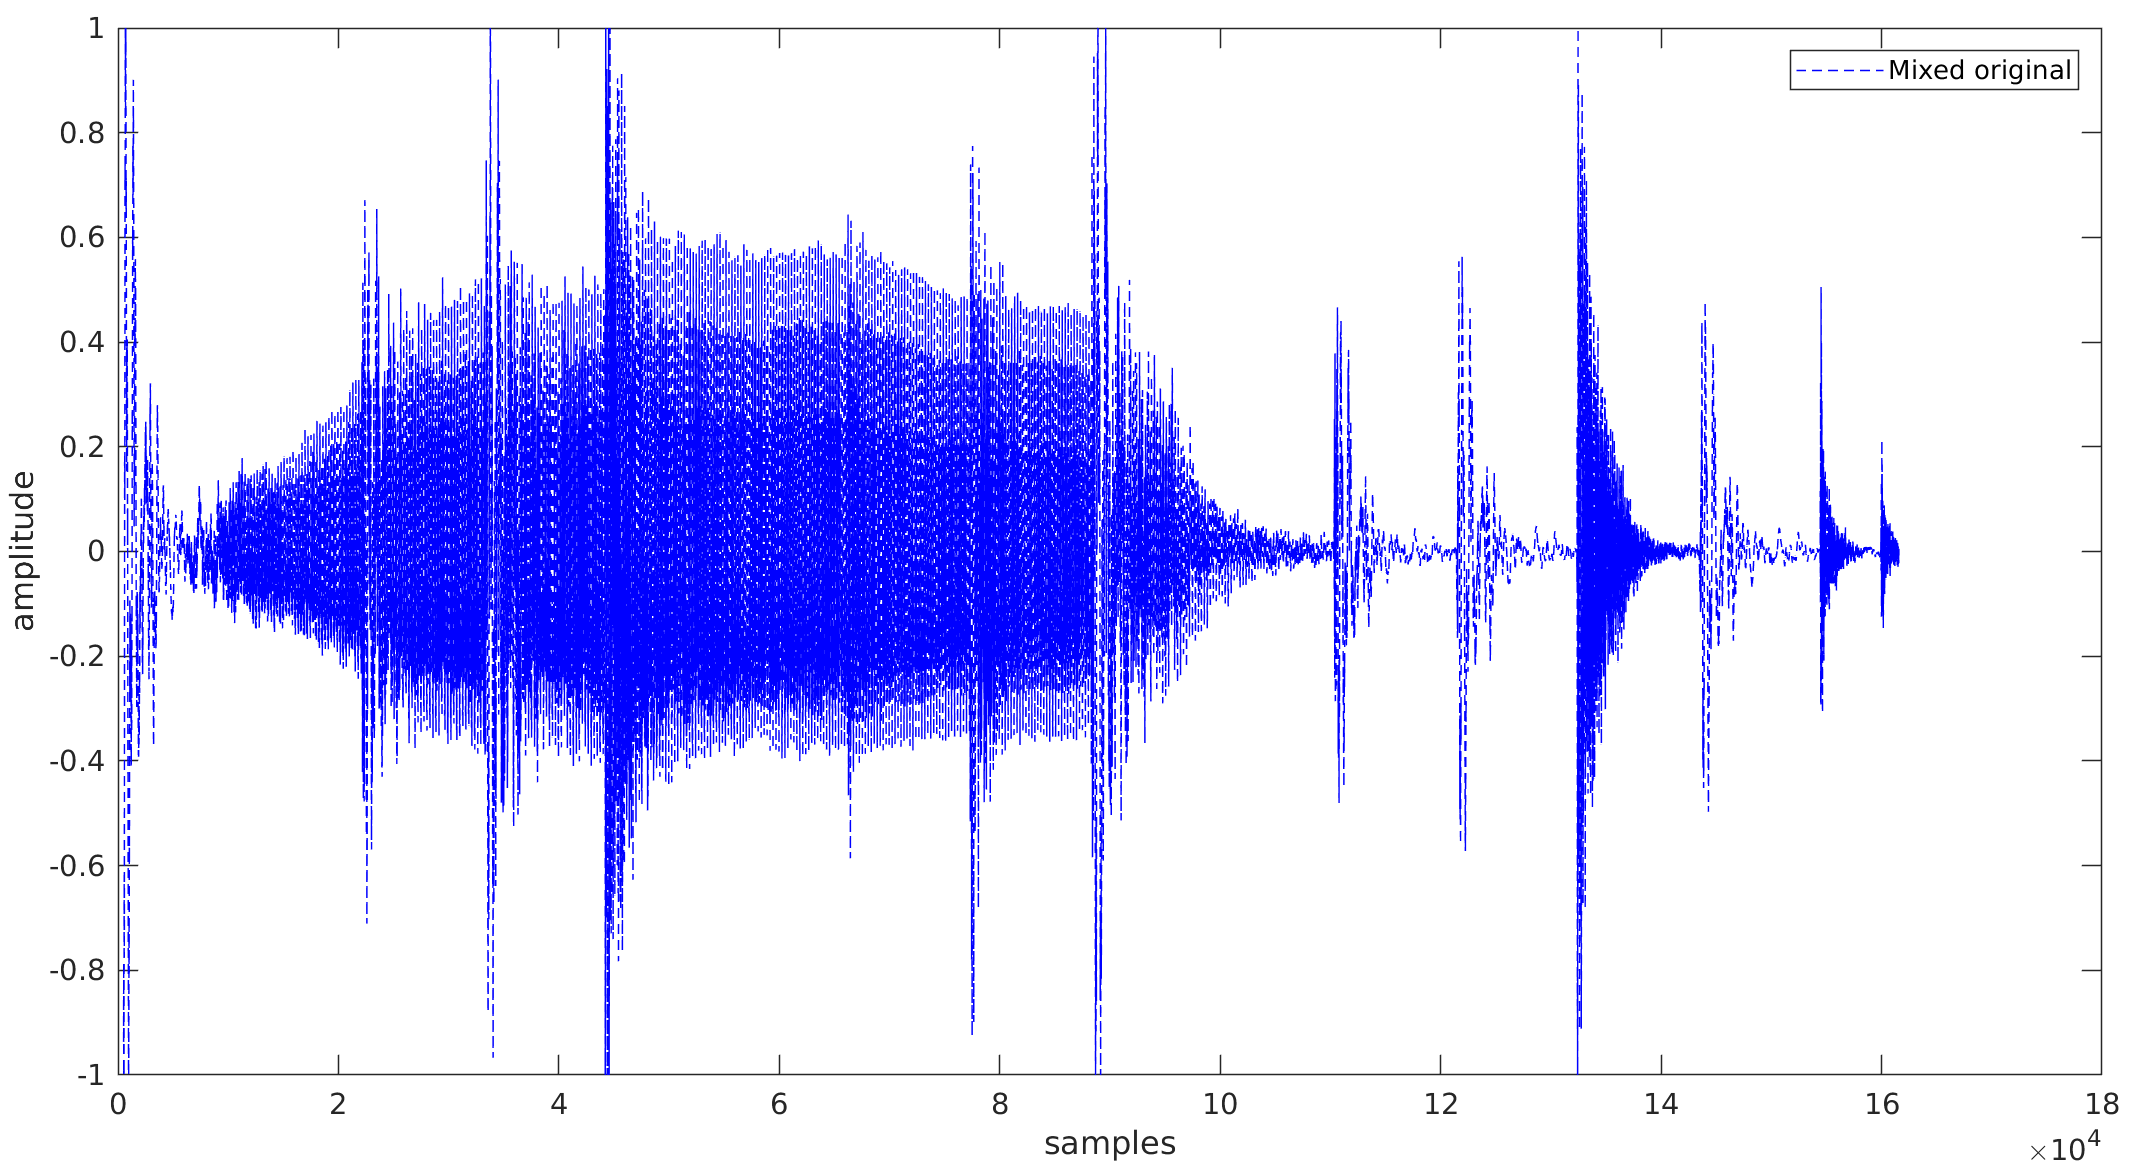
\includegraphics[width=12cm]{../images/waveform_realtime_orig.png} }}
	\\
	\subfloat[Harmonic waveforms, separated vs. original]{{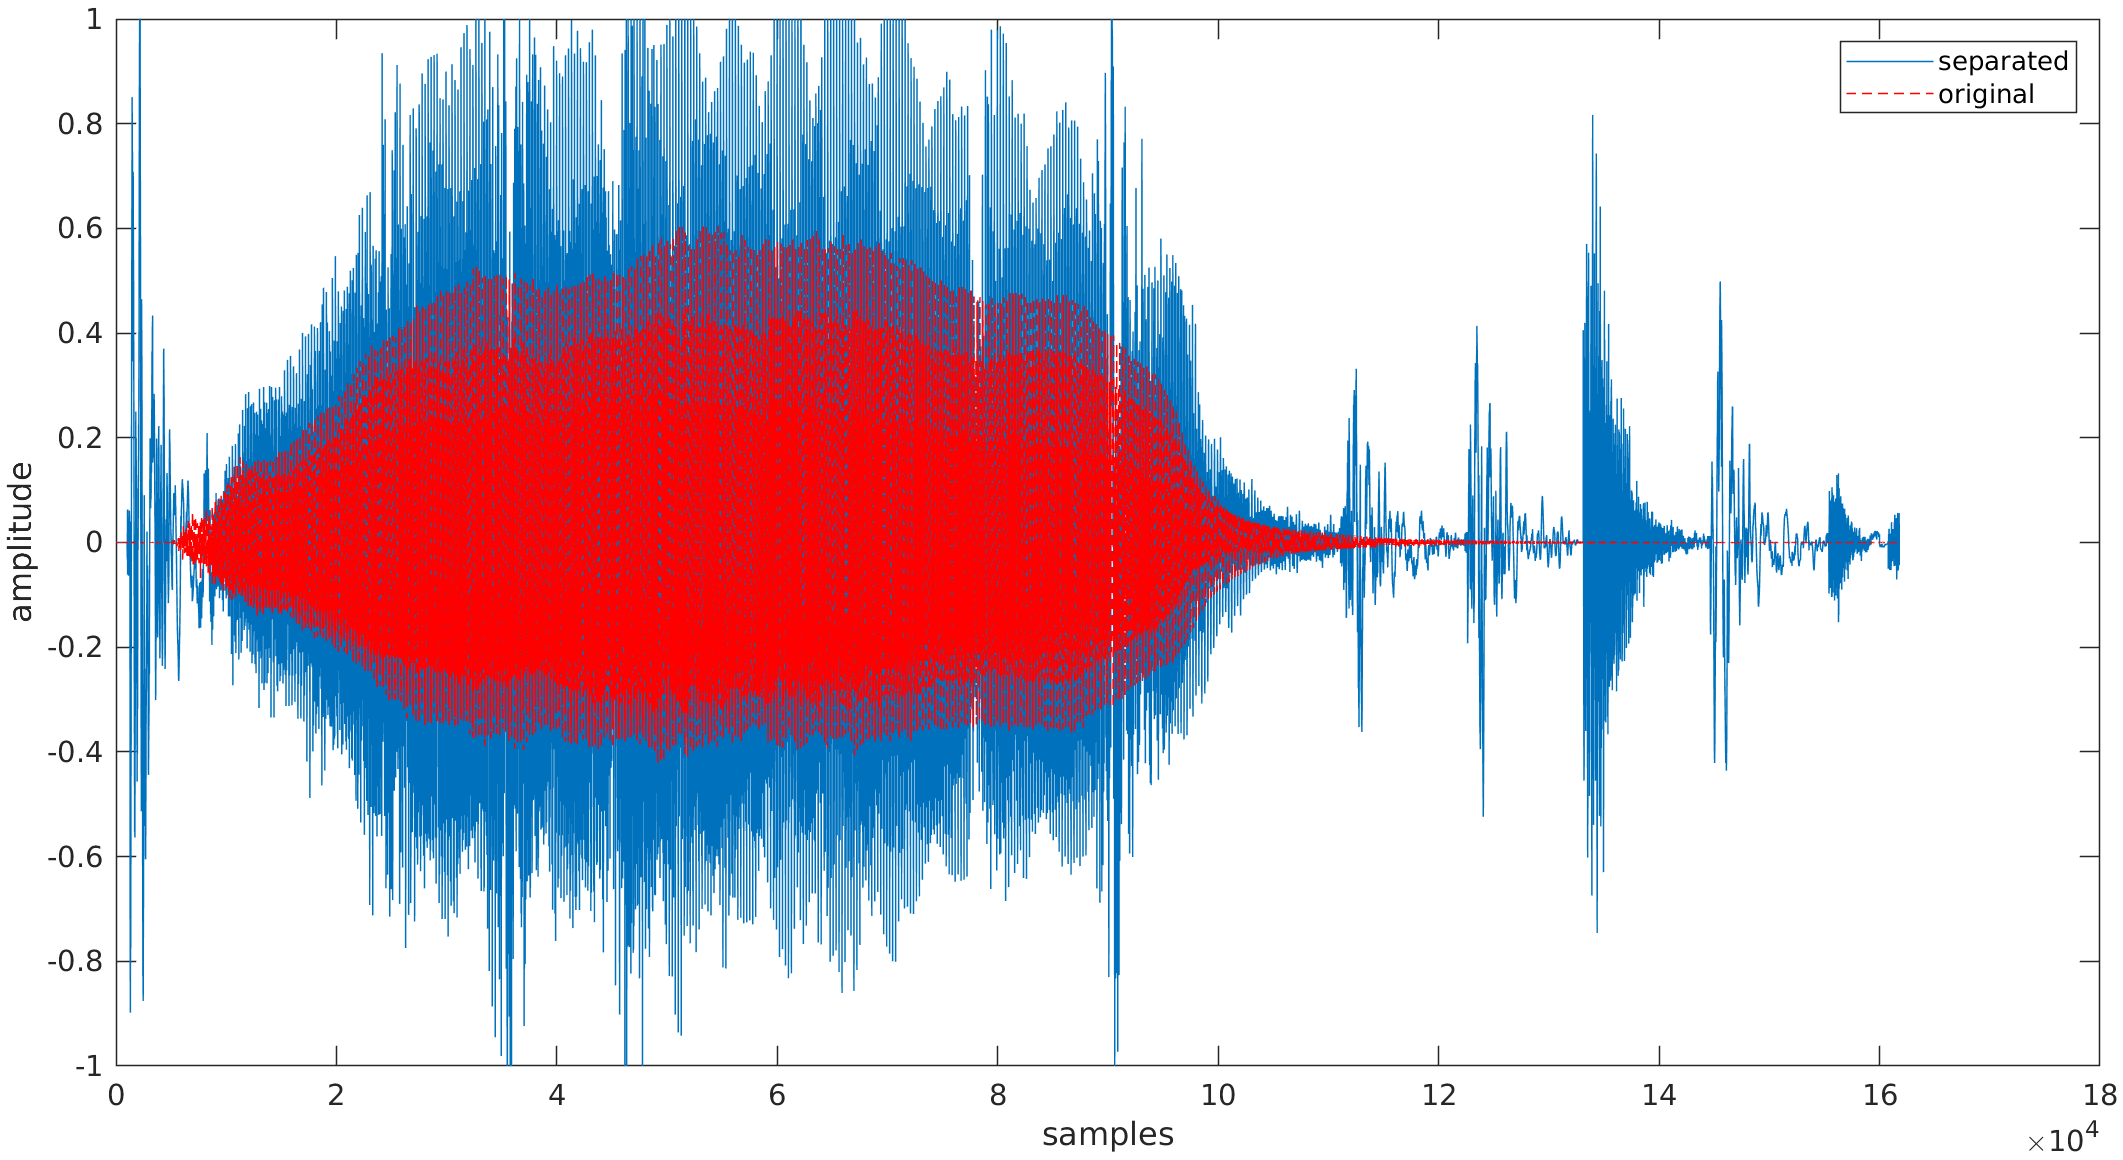
\includegraphics[width=12cm]{../images/harm_realtime_cmp.png} }}
	\\
	\subfloat[Percussive waveforms, separated vs. original]{{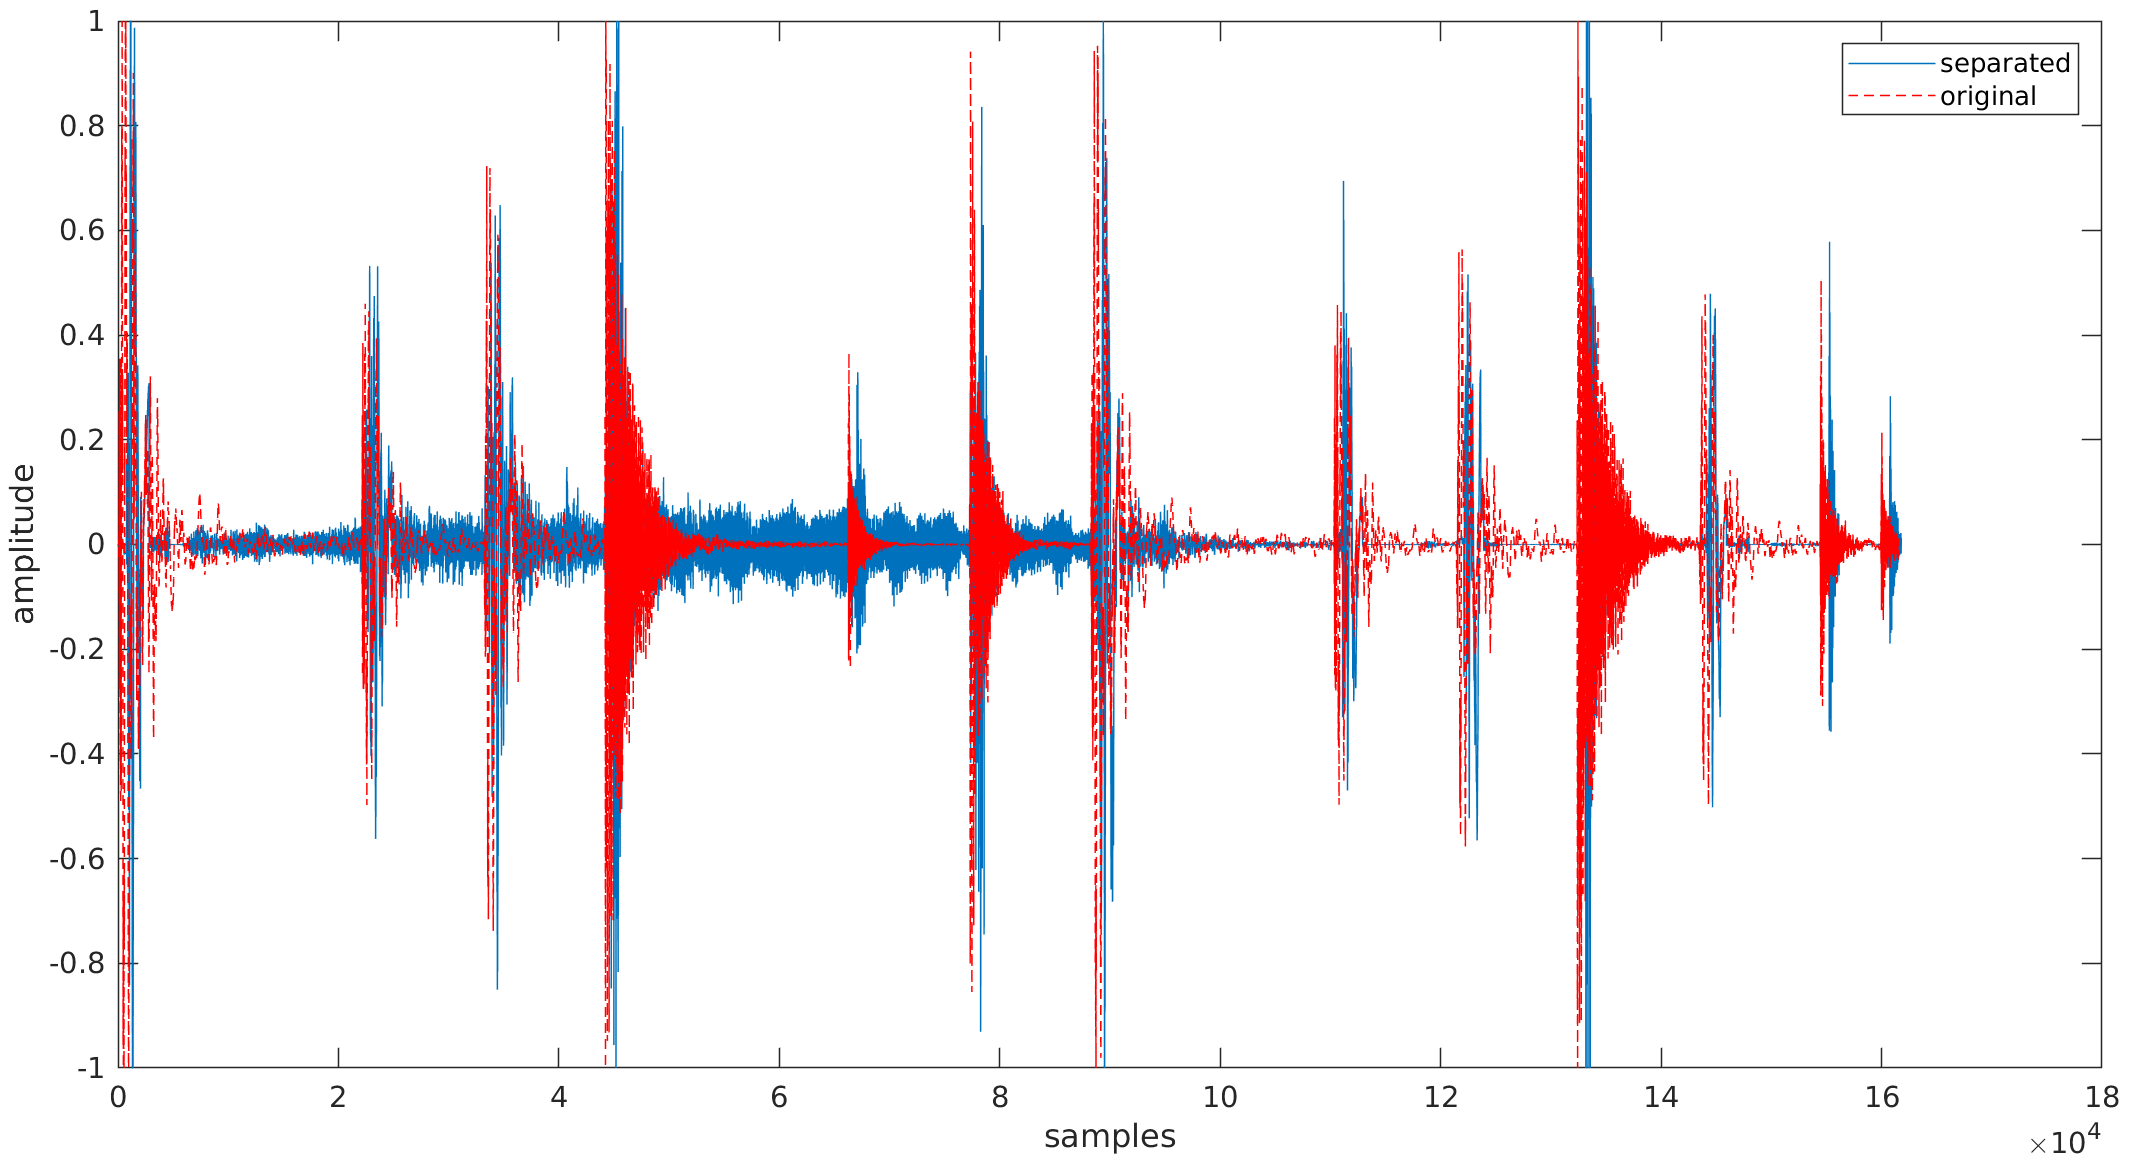
\includegraphics[width=12cm]{../images/perc_realtime_cmp.png} }}
	\caption{Real-time HPSS results, time-domain waveform}
	\label{fig:rtresults1}
\end{figure}

\begin{figure}[ht]
	\centering
	\subfloat[Mix spectrogram]{{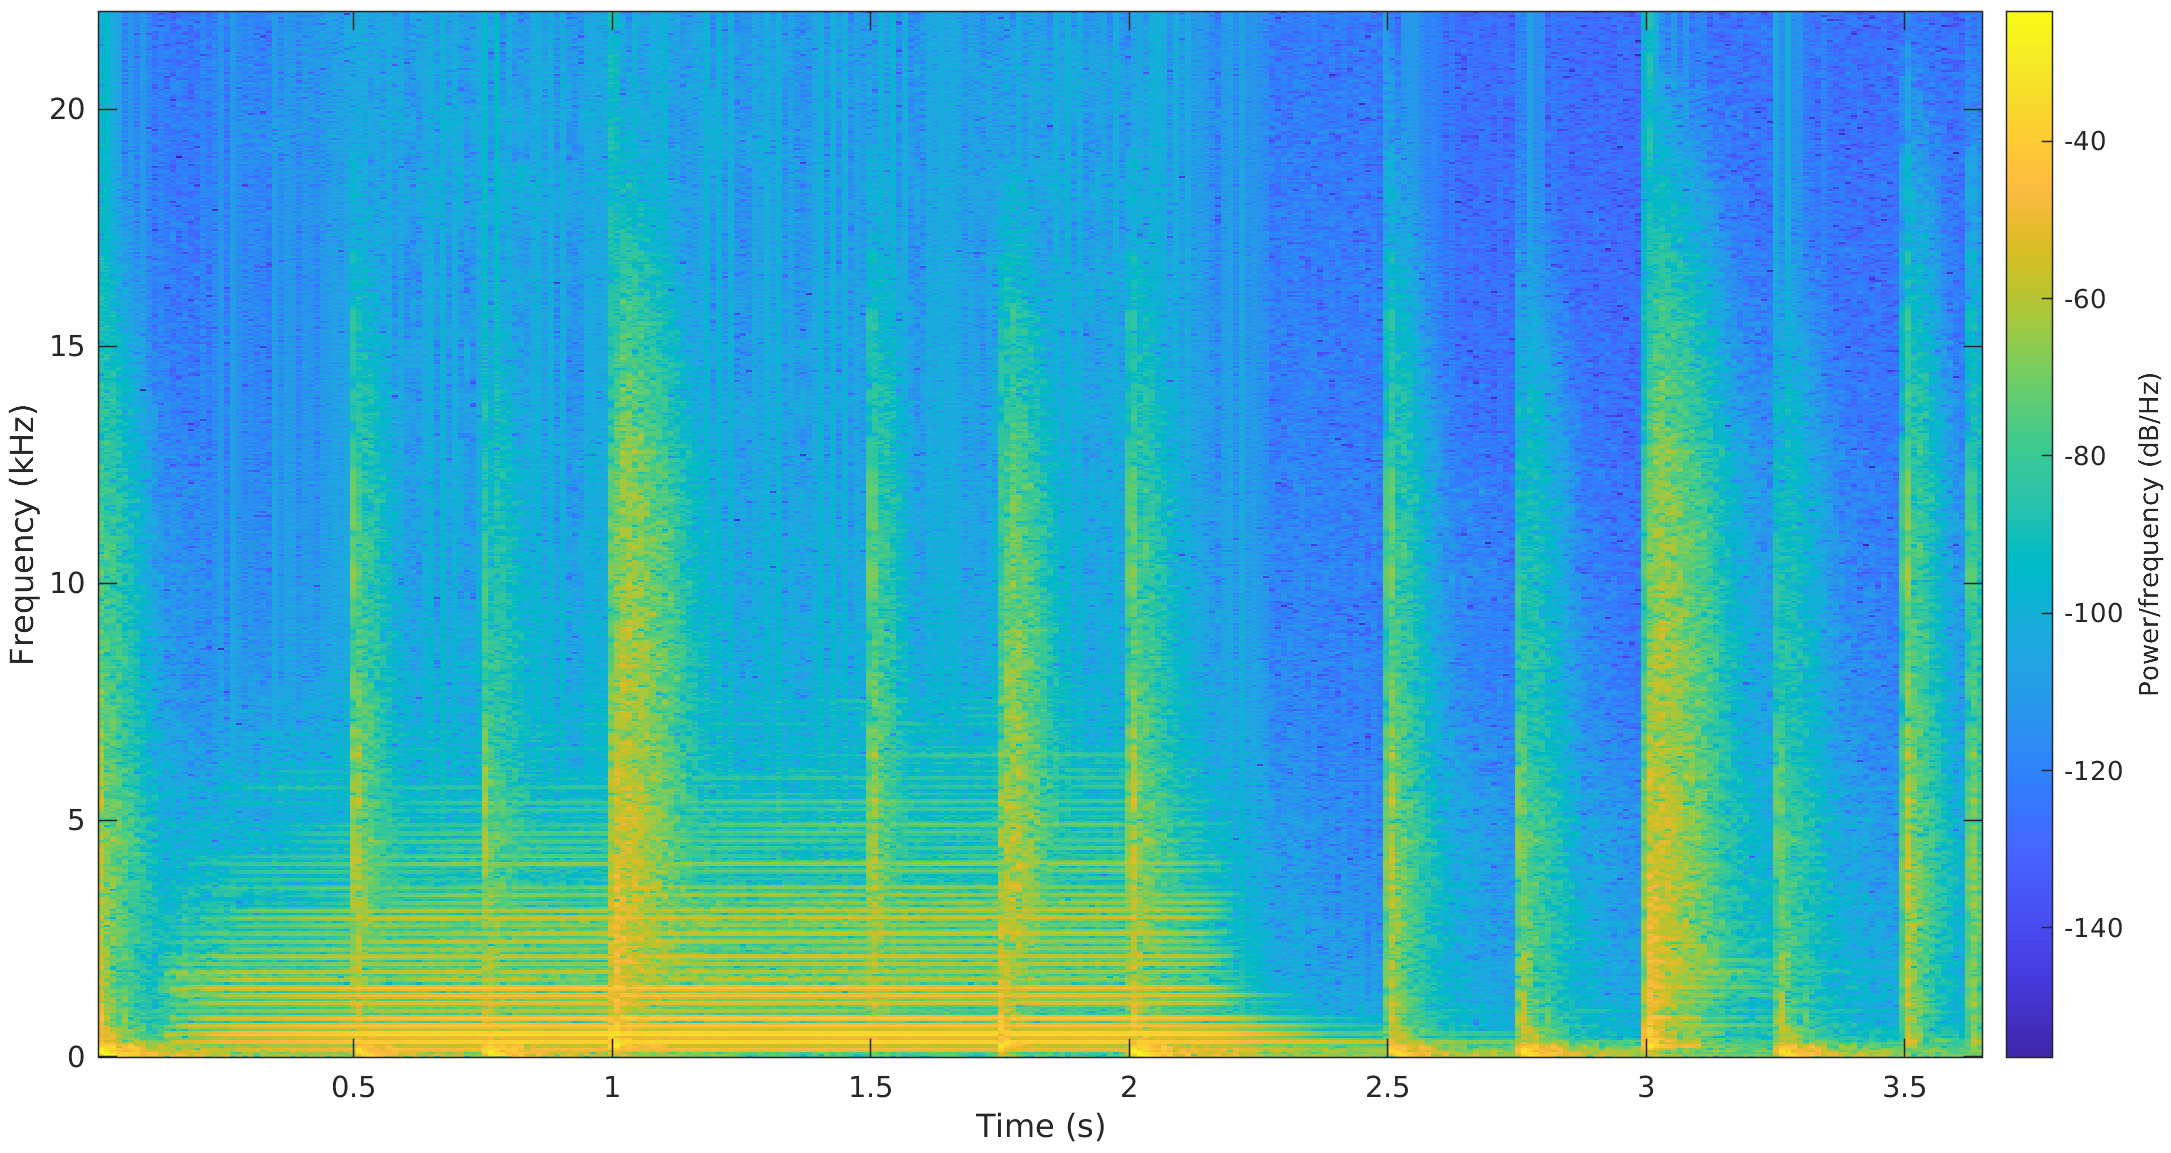
\includegraphics[width=12cm]{../images/mixedspecgram.png} }}
	\\
	\subfloat[Harmonic recovered spectrogram]{{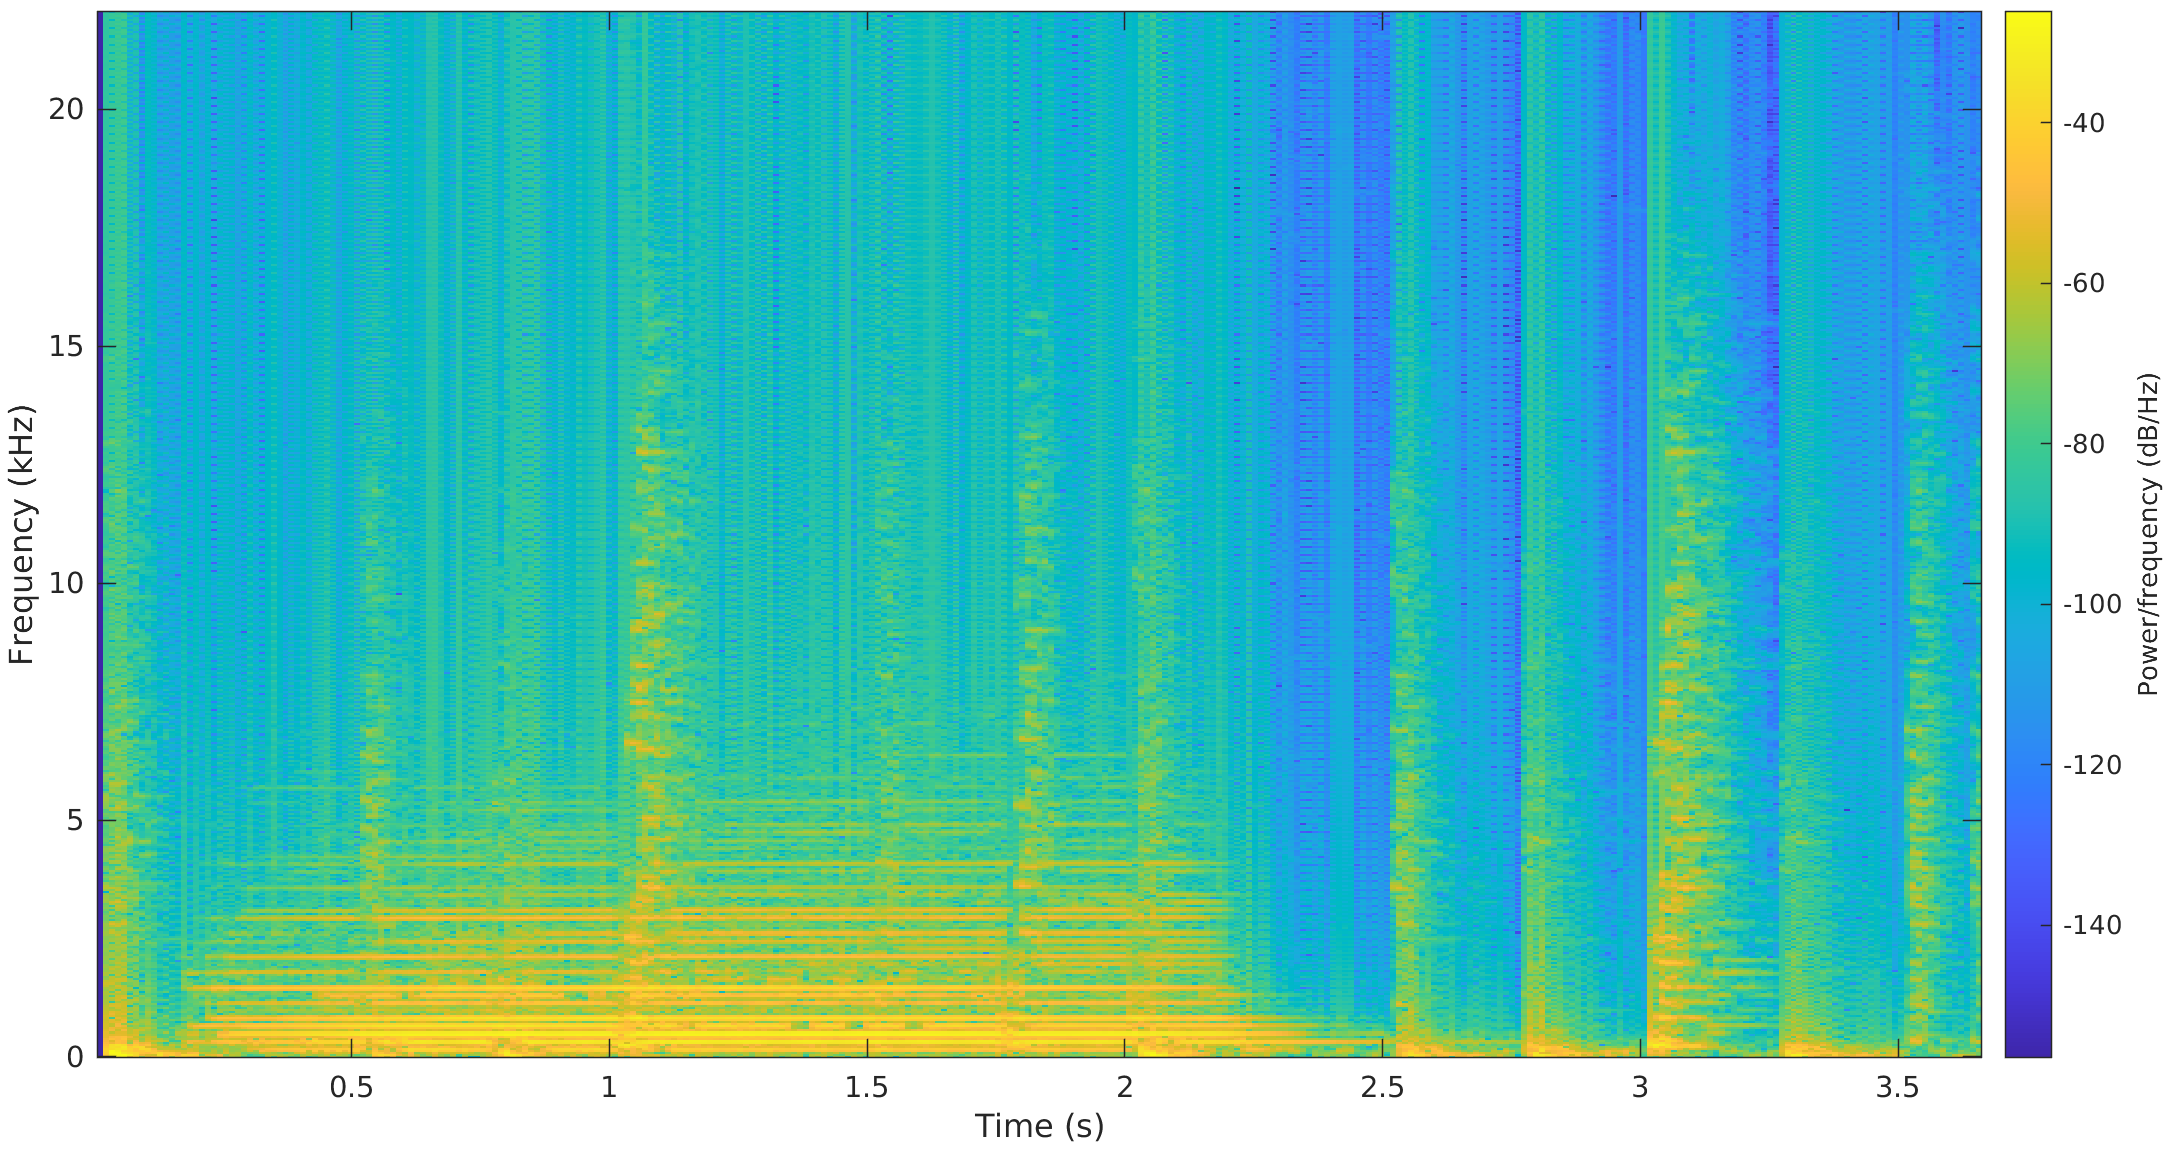
\includegraphics[width=12cm]{../images/harm_realtime.png} }}
	\\
	\subfloat[Percussive recovered spectrogram]{{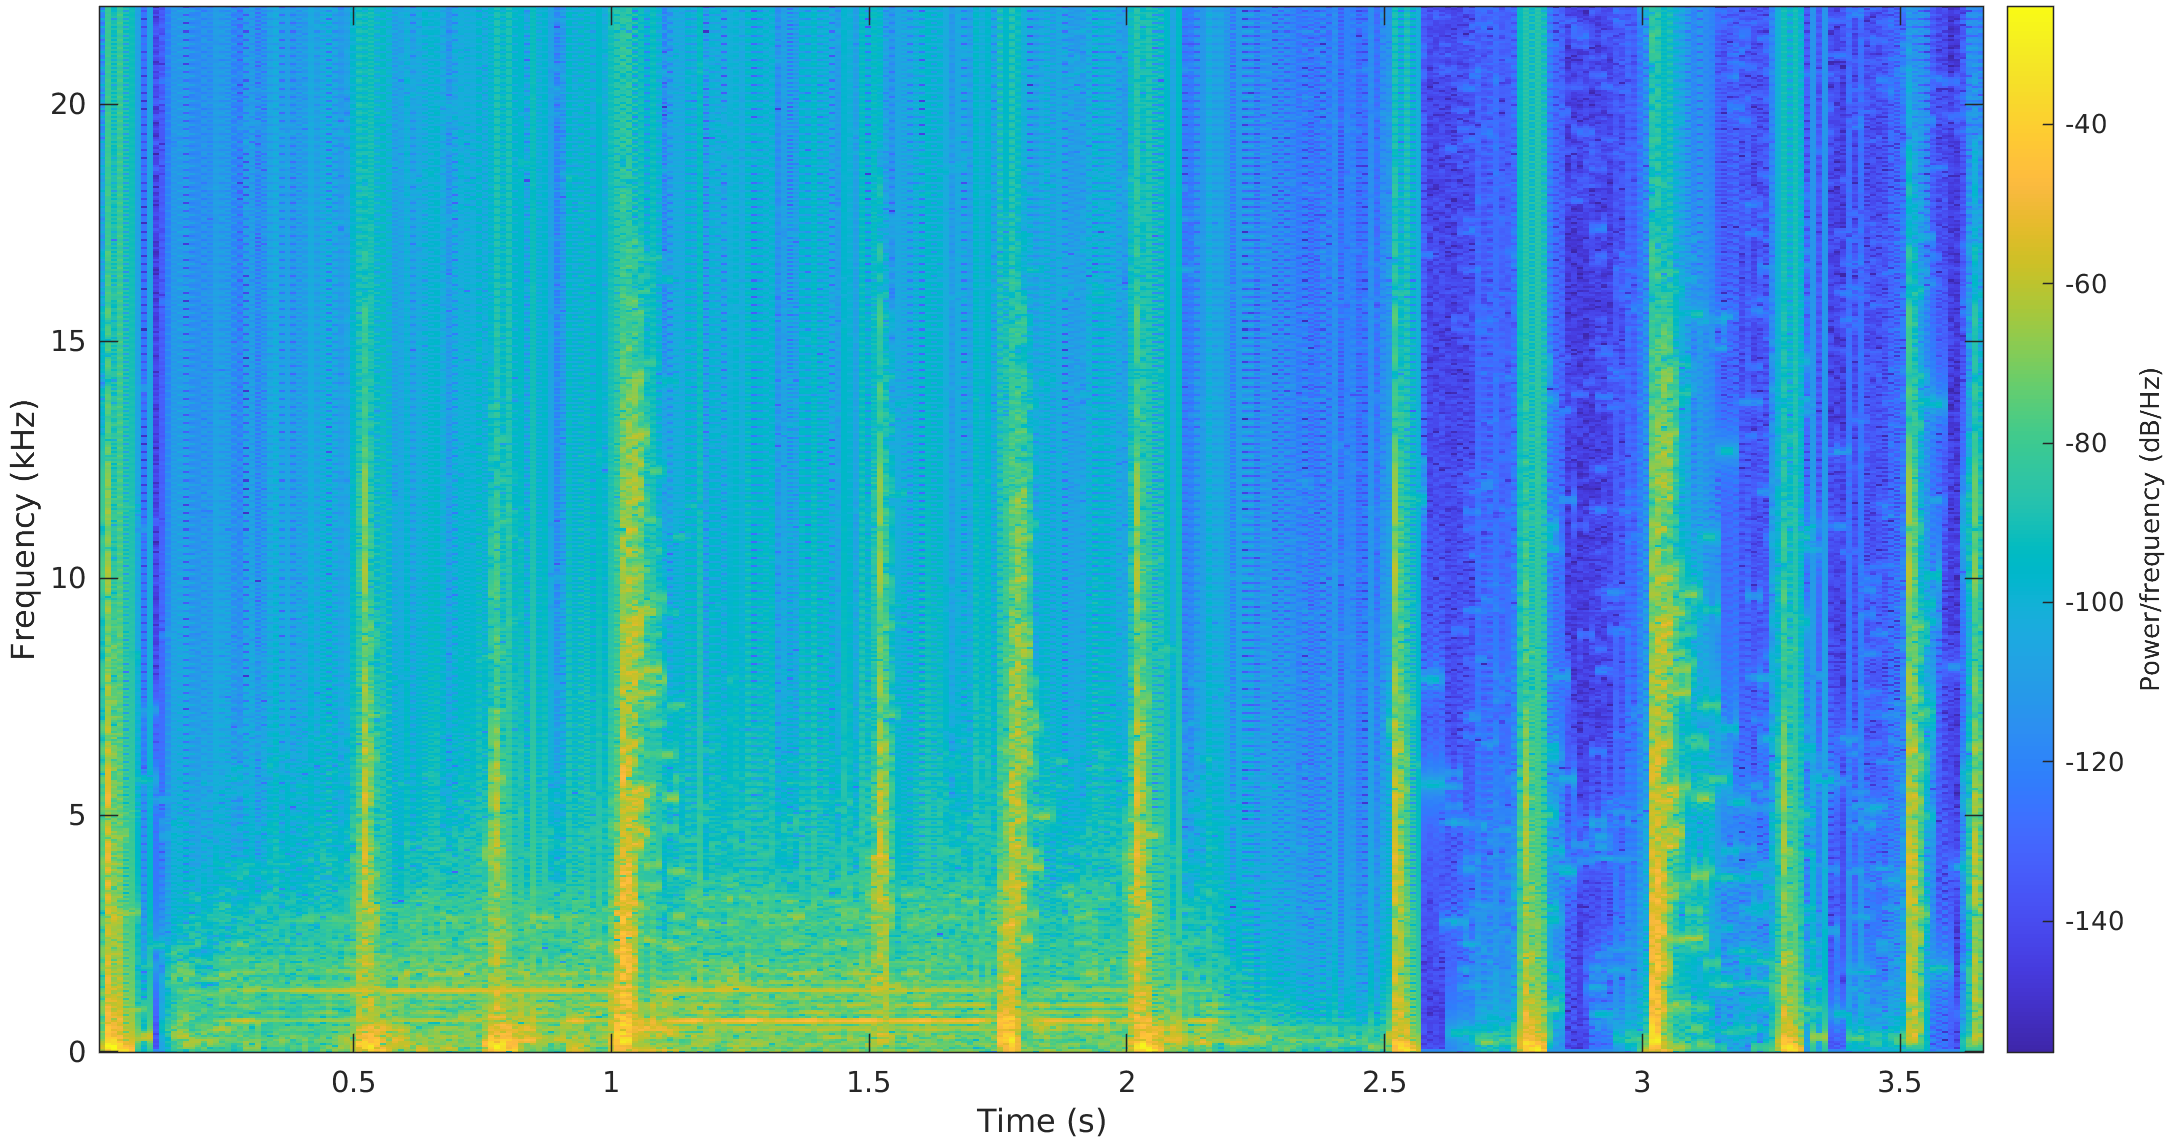
\includegraphics[width=12cm]{../images/perc_realtime.png} }}
	\caption{Real-time HPSS results, spectrograms}
	\label{fig:rtresults2}
\end{figure}

\vfill
\clearpage %force a page break

Finally, Figure~\ref{fig:rtresults3} shows a 3-way comparison between the original harmonic and percussive waveforms, and the separations performed using the Driedger et al. HPSS algorithm with $\beta = 2$ in the regular/offline variant of Listing~\ref{code:fullimpl}, and my real-time version of Listing~\ref{code:rtimpl}. From the figures it is apparent that the harmonic real-time separation is rather poor. This fits the prediction that missing the forward/future half of the STFT median filter would adversely affect harmonic separation in the real-time variant.\\

In the percussive separation, the remnants of the viola note (from 20,000 -- 100,000 samples) is bigger in the real-time HPSS, meaning it performed a worse separation. Initially, I predicted that the percussive separation would be identical in the real-time variant. However, the detail I missed is that the percussive and harmonic separations are interdependent in the mask calculation, so a worse harmonic separation will affect the quality of the percussive separation.

\begin{figure}[ht]
	\centering
	\subfloat[Harmonic waveforms]{{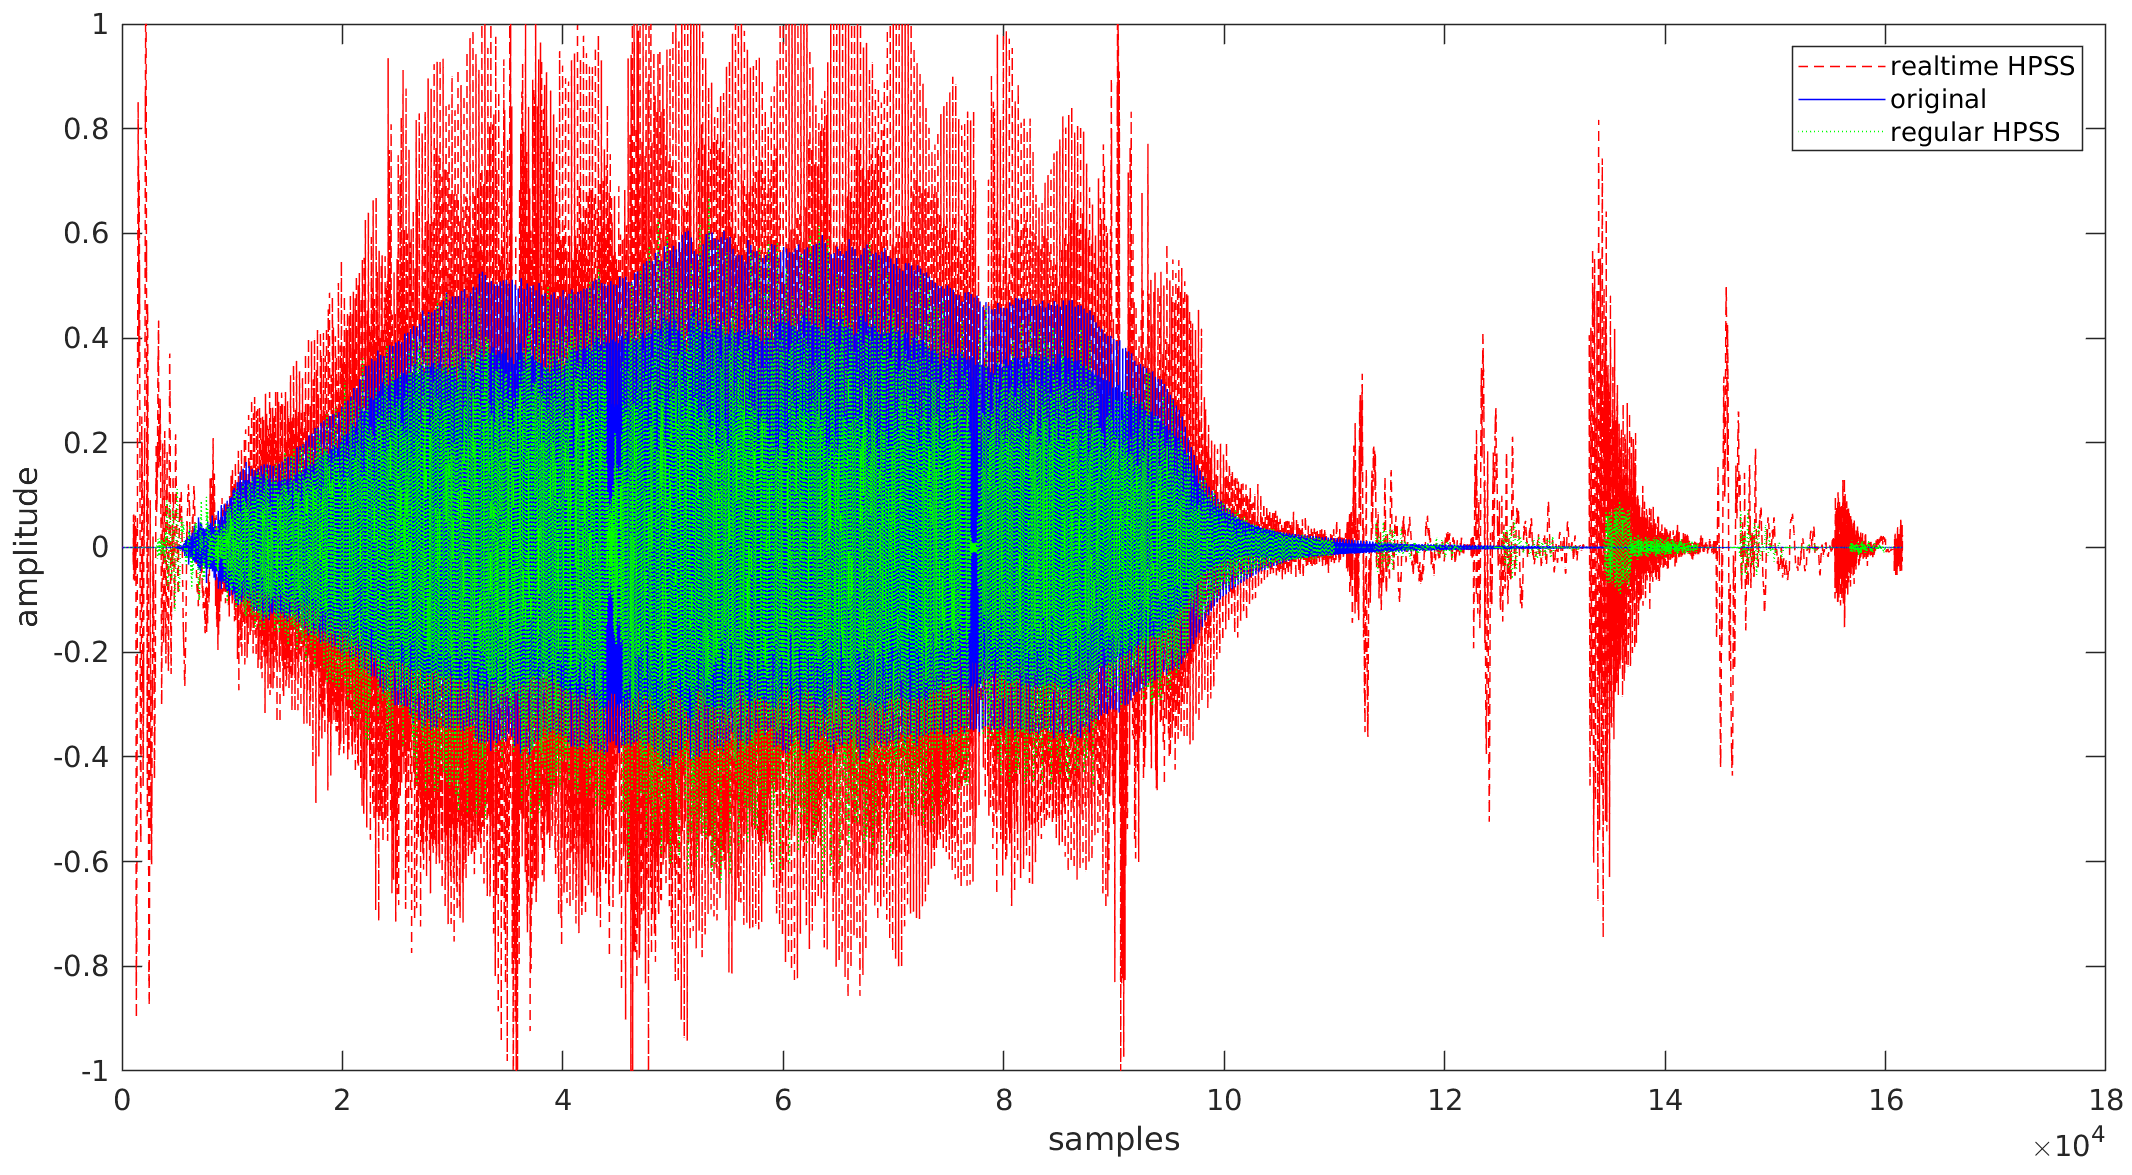
\includegraphics[width=12cm]{../images/harm_3way.png} }}
	\\
	\subfloat[Percussive waveforms]{{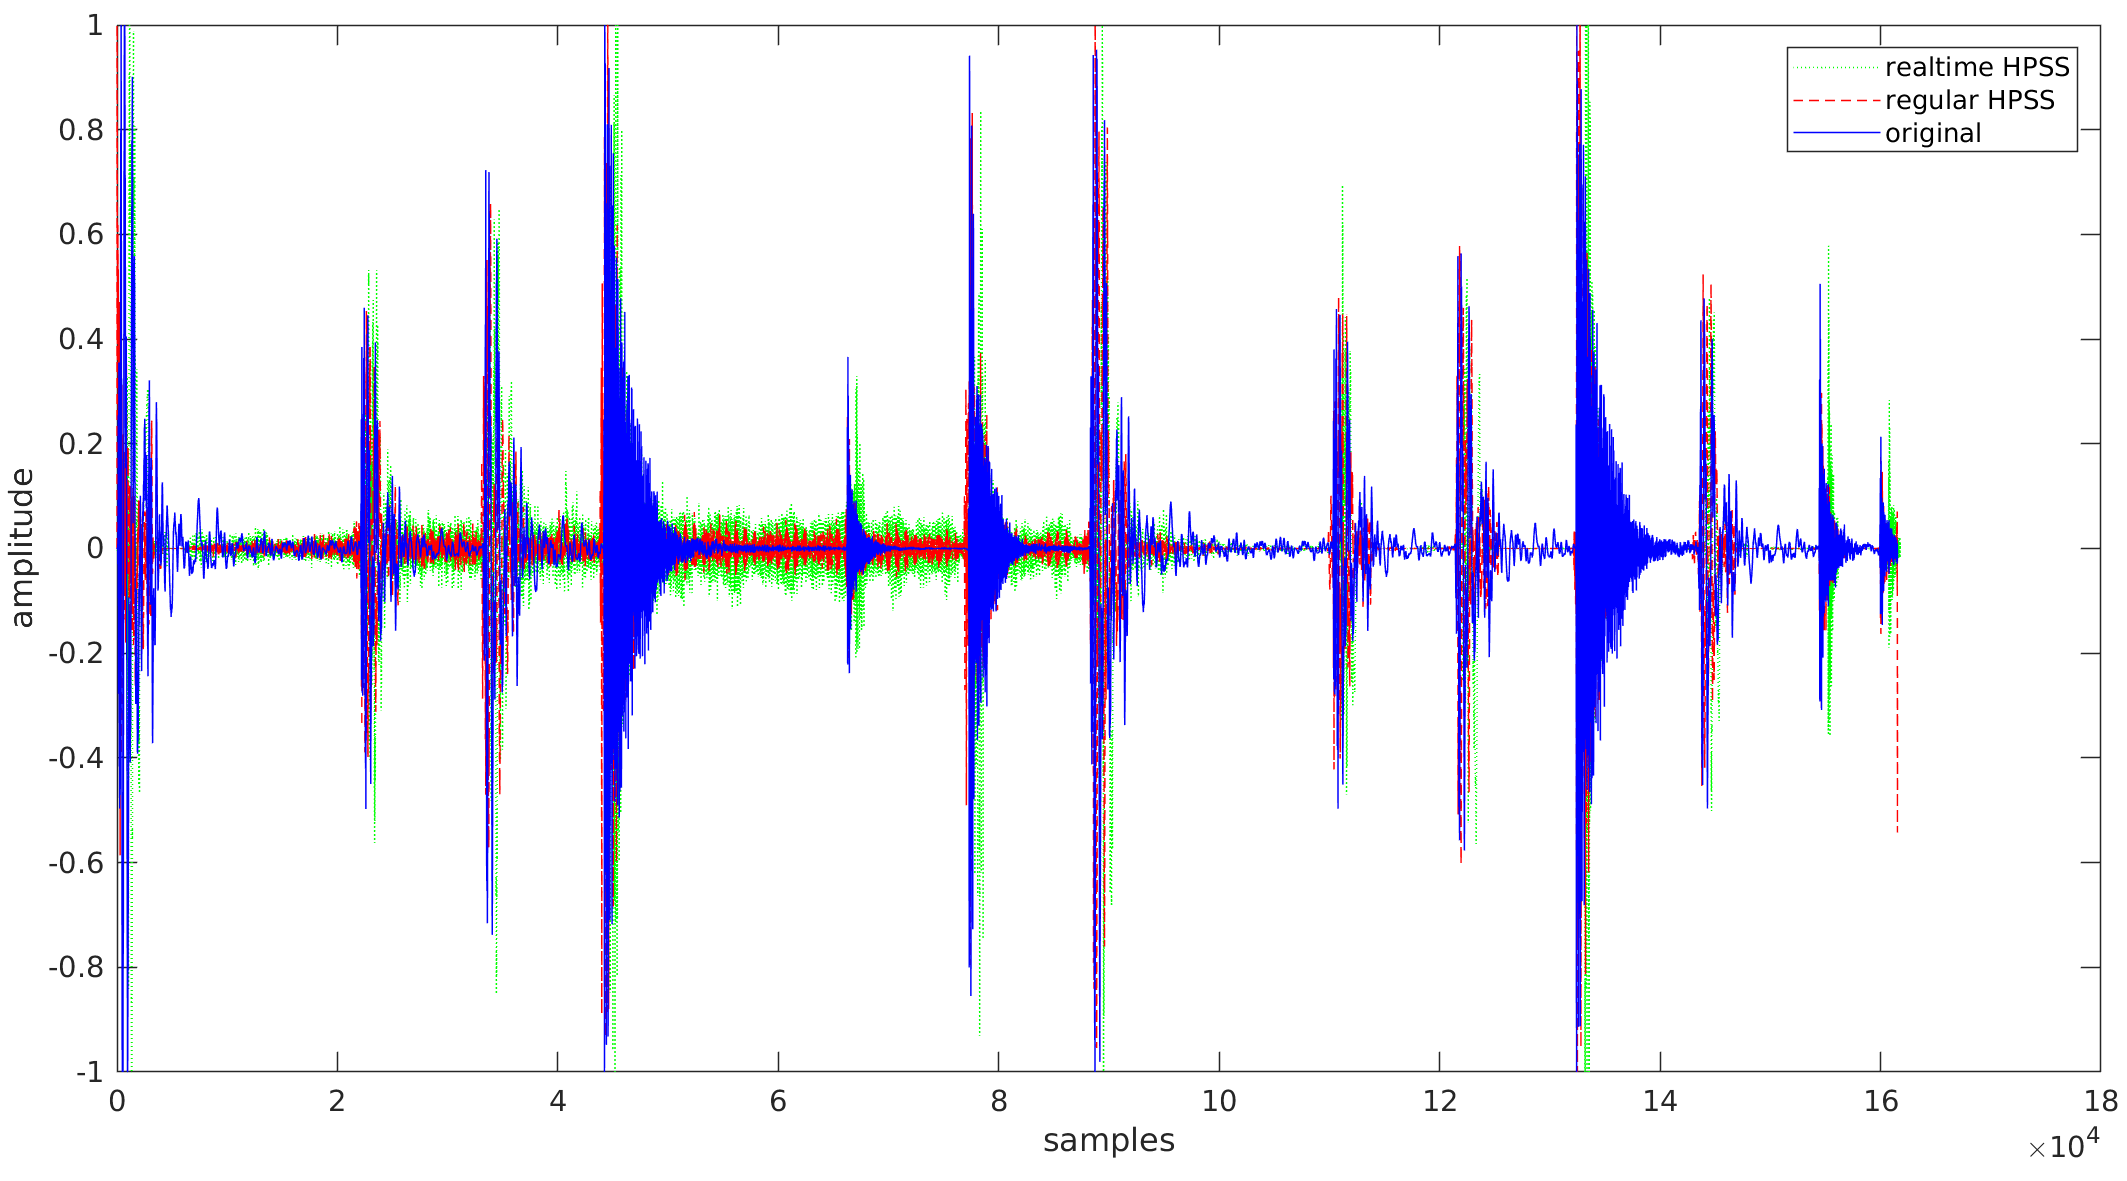
\includegraphics[width=12cm]{../images/perc_3way.png} }}
	\caption{3-way comparison, original vs. real-time HPSS vs. regular HPSS}
	\label{fig:rtresults3}
\end{figure}

\vfill
\clearpage %force a page break

\subsection{Python implementation}

As a final step, to demonstrate that the real-time HPSS algorithm created in MATLAB is generally applicable, a prototype in Python was developed using numpy and scipy. As usual, the code is available at \url{https://github.com/sevagh/Real-Time-HPSS}. The real-time HPSS is implemented as a class, ``HPSSRT'', which when passed single $hop$-sized numpy.ndarrays to process, returns a tuple of $hop$-sized $h$ and $p$. The spectrograms in Figure~\ref{fig:pyresults} on the next page were created the same mixed viola and drum clip throughout the paper, processed in $hop$-sized chunks using the ``HPSSRT'' Python class and the Python code in Listing~\ref{code:matplotlib} below.

\begin{listing}[h]
\setlength\partopsep{-\topsep}
\begin{minted}[breaklines,linenos,frame=single,fontsize=\small,linenos]{python}
import scipy
import scipy.signal
import scipy.io.wavfile
import matplotlib.pyplot as plt
import numpy
from hpss_rt import HPSSRT

fs, x = scipy.io.wavfile.read("mixed.wav")
hpss = HPSSRT(fs)

h = numpy.ndarray(shape=x.shape)
p = numpy.ndarray(shape=x.shape)

x_ptr = 0
while x_ptr < len(x):
    if len(x[x_ptr : x_ptr + hpss.hop]) != hpss.hop:
        # skip uneven/non-hop-sized last chunk
        break
    h_, p_ = hpss.process_next_hop(x[x_ptr : x_ptr + hpss.hop])
    h[x_ptr : x_ptr + hpss.hop] = h_
    p[x_ptr : x_ptr + hpss.hop] = p_
    x_ptr += hpss.hop

scipy.io.wavfile.write("h_rt_sep_python.wav", fs, h)
scipy.io.wavfile.write("p_rt_sep_python.wav", fs, p)

fs, xm = scipy.io.wavfile.read("mixed.wav")
fs, xh = scipy.io.wavfile.read("h_rt_sep_python.wav")
fs, xp = scipy.io.wavfile.read("p_rt_sep_python.wav")
_, _, _, im = plt.specgram(xm, Fs=fs, NFFT=1024, noverlap=512)
plt.show()
_, _, _, im = plt.specgram(xh, Fs=fs, NFFT=1024, noverlap=512)
plt.show()
_, _, _, im = plt.specgram(xp, Fs=fs, NFFT=1024, noverlap=512)
plt.show()
\end{minted}
\caption{Python real-time HPSS}
\label{code:matplotlib}
\end{listing}

\vfill
\clearpage %force a page break

\begin{figure}[ht]
	\centering
	\subfloat[Mixed spectrogram]{{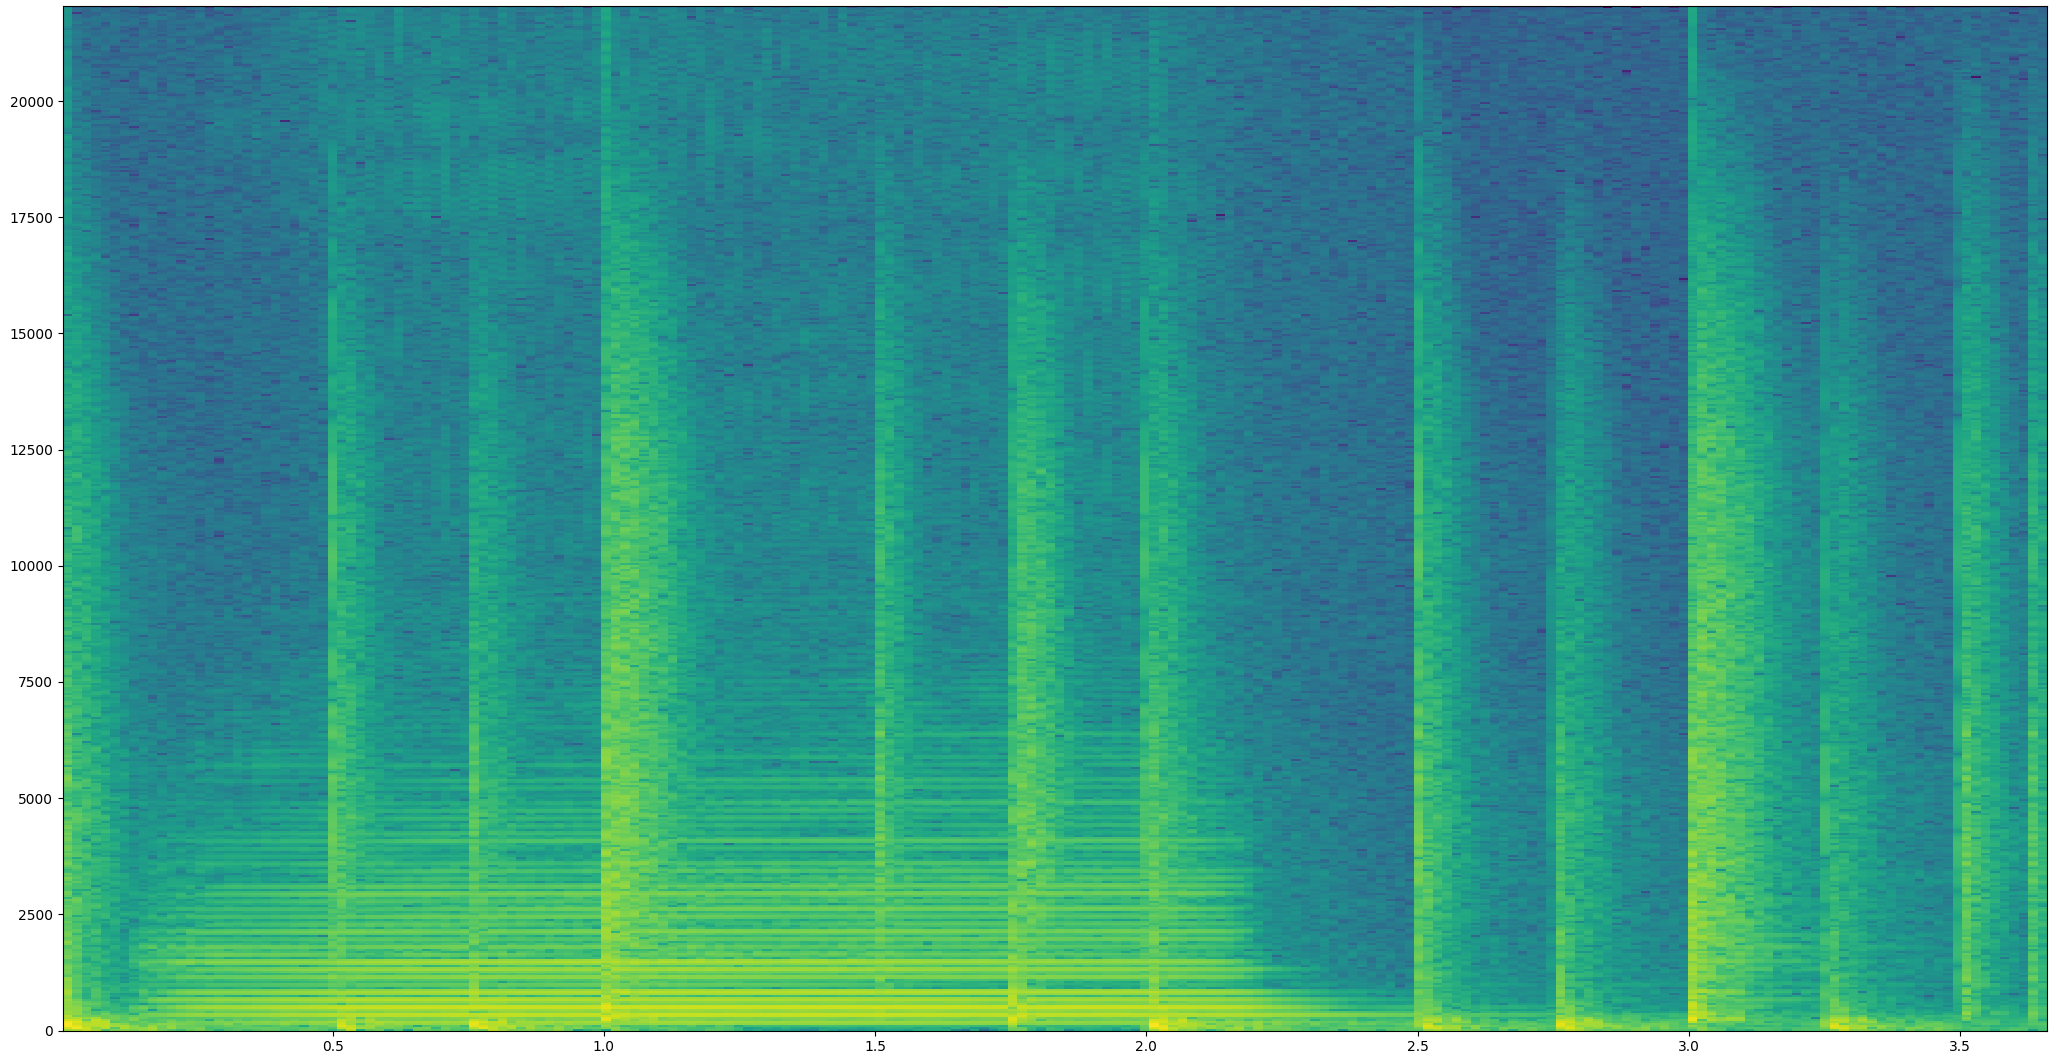
\includegraphics[width=12cm]{../images/mixed_specgram_matplotlib.png} }}
	\\
	\subfloat[Harmonic separated spectrogram]{{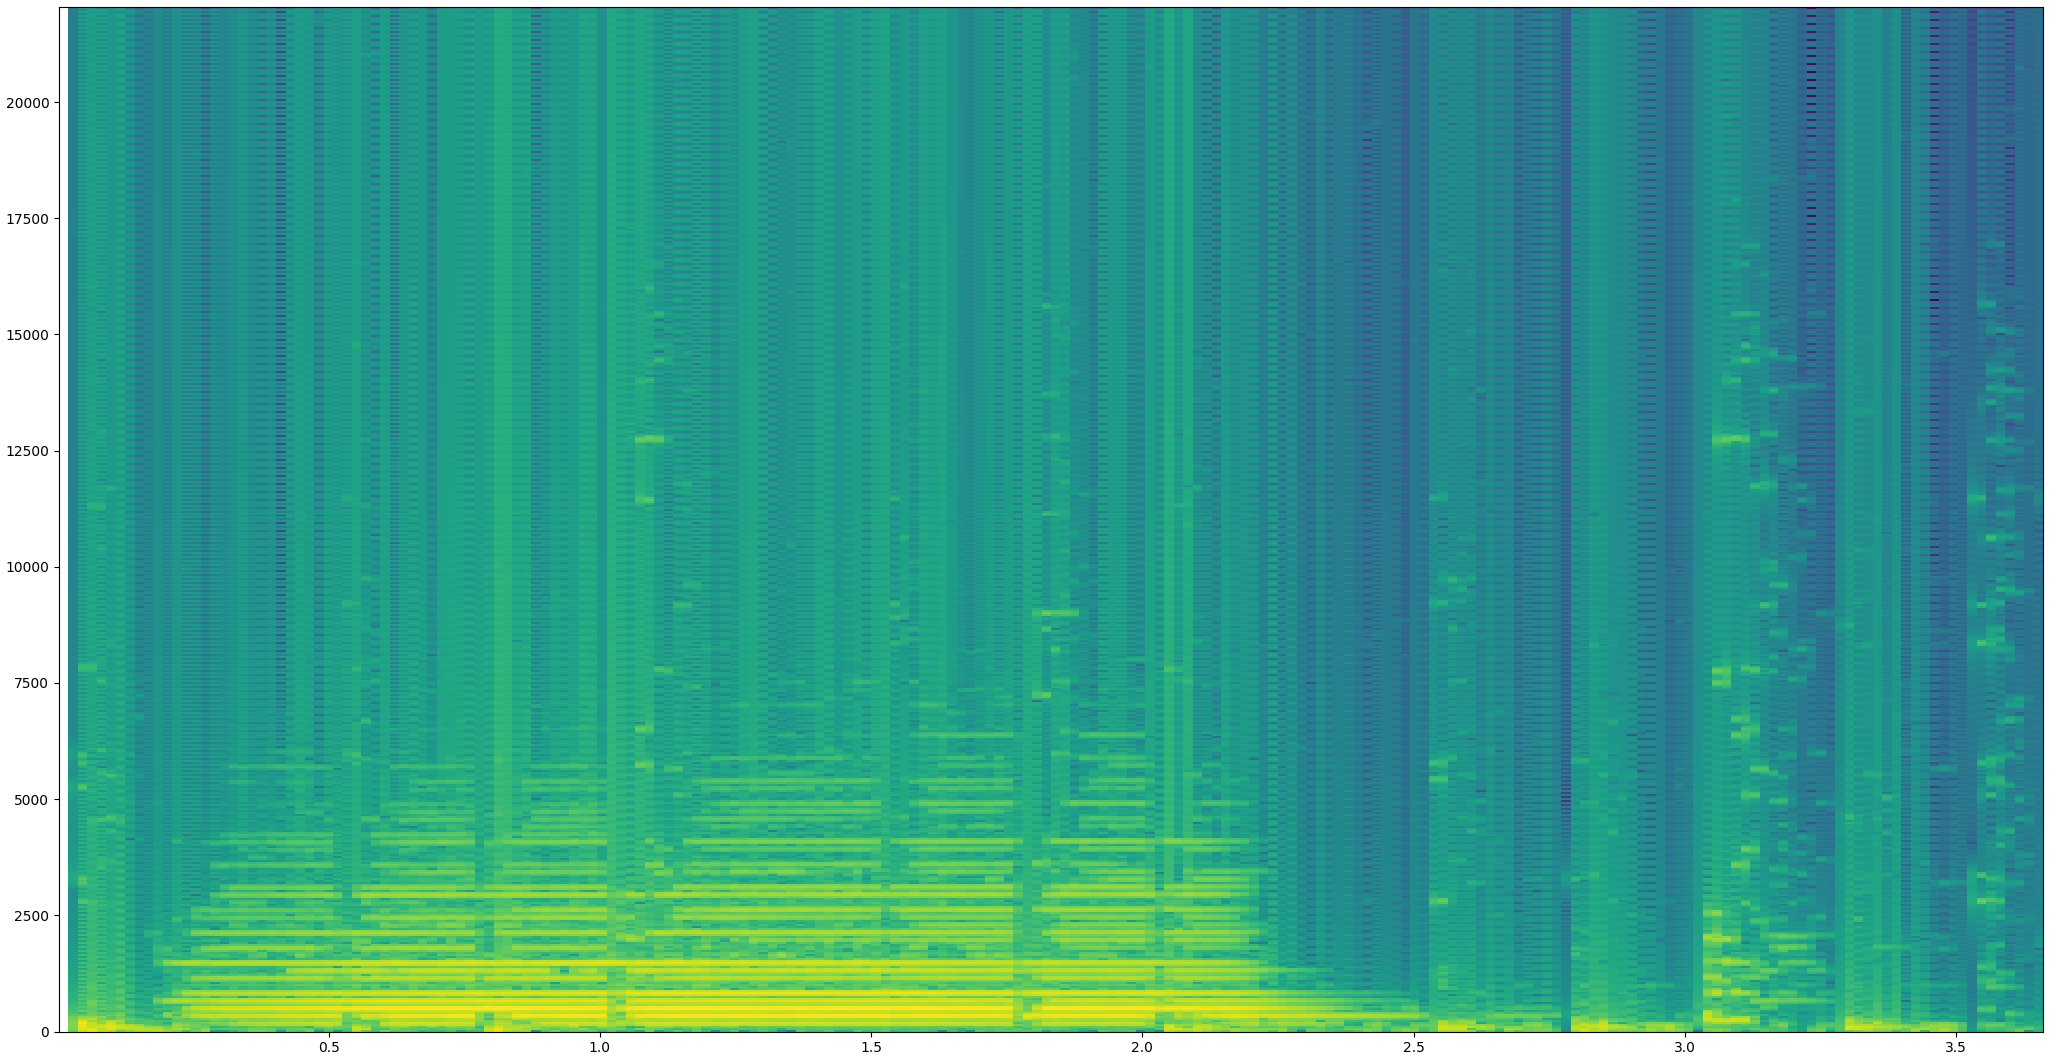
\includegraphics[width=12cm]{../images/harm_specgram_matplotlib.png} }}
	\\
	\subfloat[Percussive separated spectrogram]{{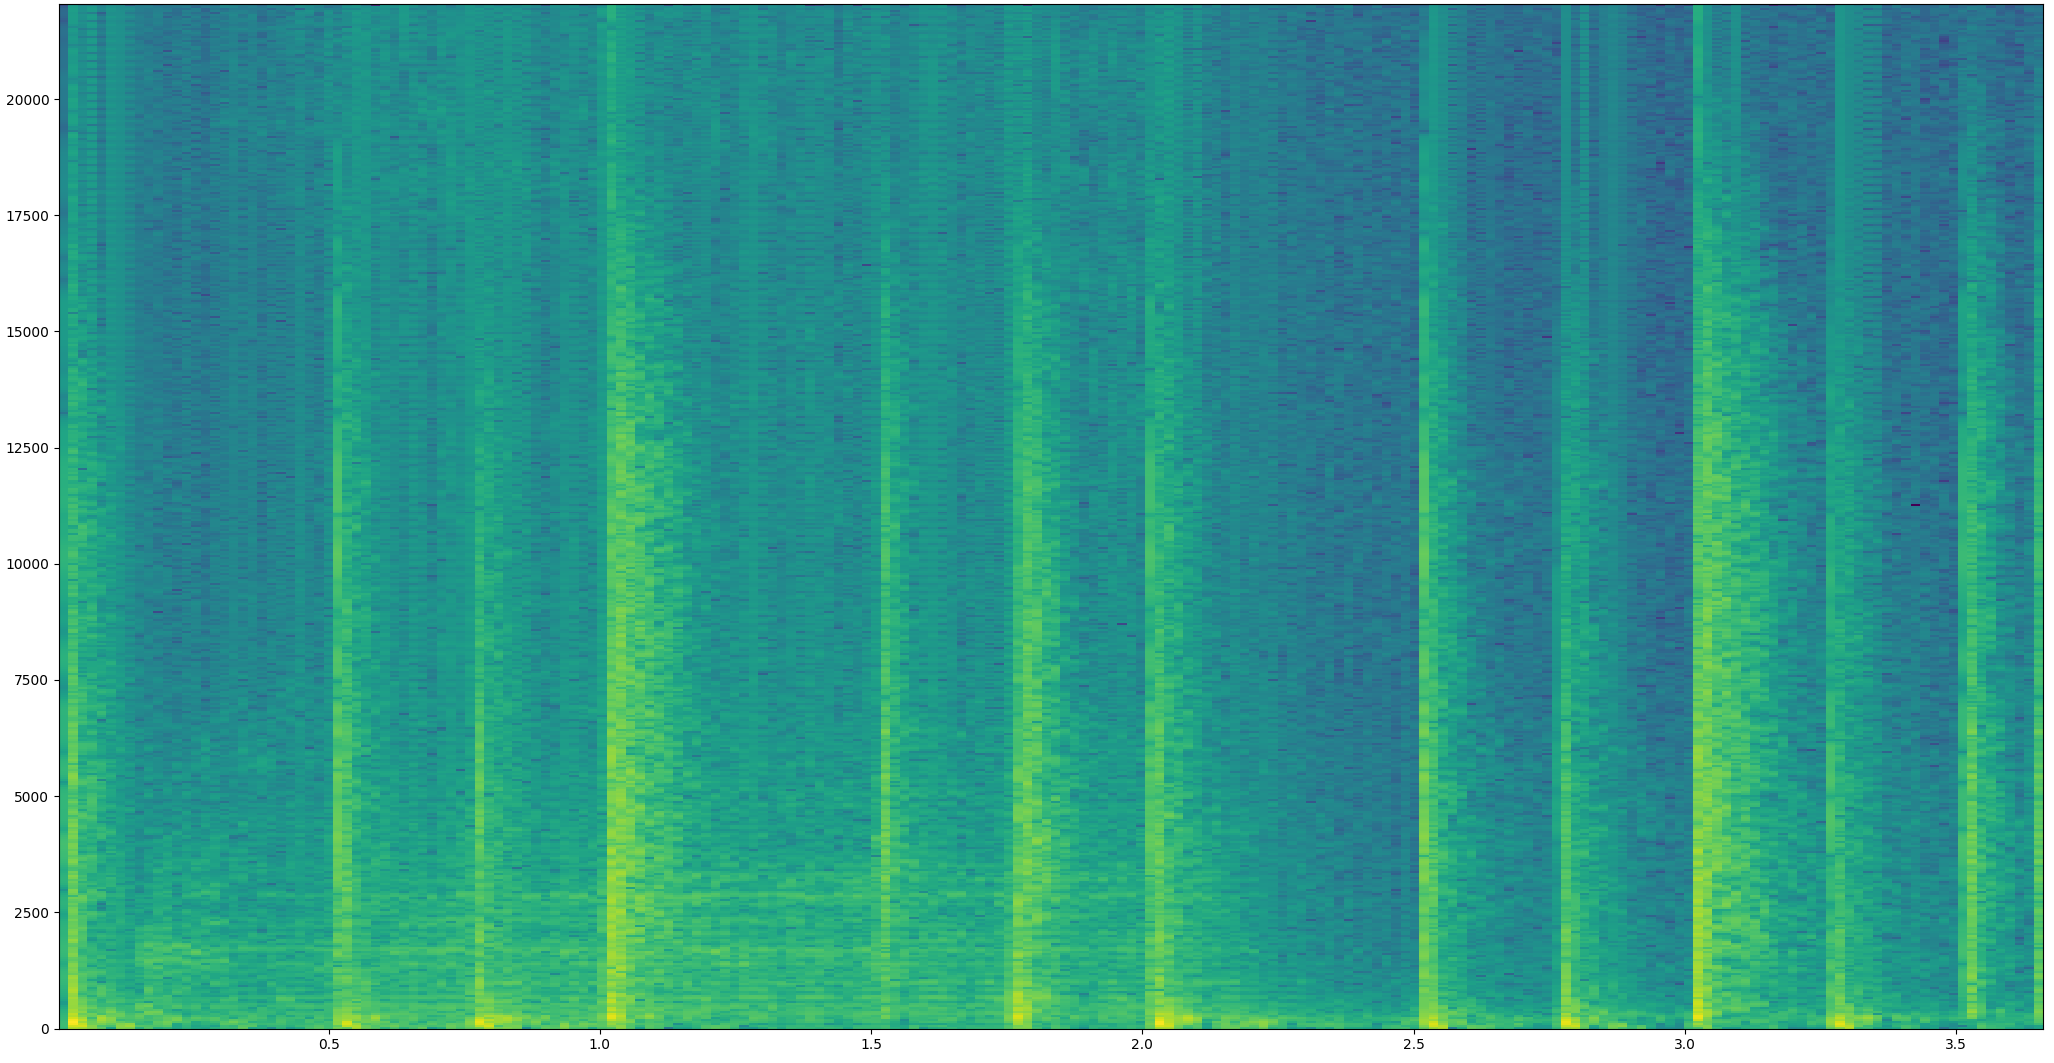
\includegraphics[width=12cm]{../images/perc_specgram_matplotlib.png} }}
	\caption{Spectrogram results of real-time HPSS in Python}
	\label{fig:pyresults}
\end{figure}

\vfill
\clearpage %force a page break

\subsection{Computation latency}

In the real-time algorithm description, latency was briefly discussed. We get a harmonic and percussive separated frames of size 512 for every input frame of size 512, which represents 11.6ms of audio at a 44100Hz sample rate, or 10.6ms of audio at a 48000Hz sample rate.\\

By adding loop time measurements using the tic and toc stopwatch functions of MATLAB \cite{tictoc}, the average computation time to separate a 512-sample input frame into 512-sample harmonic and percussive output frames is 0.7ms. This is roughly 6\% of the 11.6ms input buffer size.\\

The Python implementation is slower, measuring at 9ms per loop iteration. I don't consider this to be a meaningful measurement, since there are many different implementation choices. Typically one should leverage Python libraries that call to faster C and FORTRAN libraries, such as numpy or scipy, and my quick implementation is only a proof of concept, and not as optimal as it could be.\\

The conclusion that one can draw from the computation times of the implementations in this report is that low computation times are in the realm of possibility for real-time HPSS. In the future one could develop specialized and optimized C or C++ library based on the presented algorithm.

\section{Conclusion}

In this paper, median filtering in the image processing domain was discussed. It was shown how it could be applicable in the audio domain with the spectrogram and STFT, and how this relates to the problem of harmonic-percussive source separation a.k.a HPSS. Fitzgerald's original 2010 median-filtering HPSS paper \cite{fitzgerald} and Driedger et al.'s subsequent 2014 improvements \cite{driedger} were described. They were also implemented in MATLAB and results were shown.\\

Then, the HPSS algorithm was modified using properties of the STFT to be performed in real-time. It was predicted that real-time HPSS has worse harmonic separation results, but good quality percussion separation results. Finally, proof-of-concept implementations were presented in both MATLAB and Python, along with their results. These implementations demonstrate the feasability of real-time HPSS.\\

Future work could focus on writing a more optimized implementation to reduce the computational latency of real-time HPSS, or apply some modifications or heuristics to improve the harmonic separation results.

\vfill
\clearpage %force a page break

\nocite{*}
\printbibheading[title={References},heading=bibnumbered]
\printbibliography[heading=none]

\vfill
\clearpage %force a page break

\end{document}
